\documentclass[a4paper, fontsize = 8pt, landscape]{scrartcl}
\usepackage{../../../misc_files/LateX/layout_and_colours}
\makeatletter
\def\input@path{{content/lecture_summary/}{content/examples/}}
\makeatother
\graphicspath{{content/images/}{content/lecture_summary/images/}{content/examples/images/}}

\title{Computertechnik 2}
\author{Jil Zerndt}
\date{FS 2025}

\createtitlepagestyle
\createmainpagestyle
\begin{document}
\begin{multicols}{2}
	\thispagestyle{TitlePageStyle}
	\maketitle
	\sffamily
	%TODO: fuck coding guidelines, add C reference Card to end of summary!!!
	\section{Microcontroller Basics}

\subsection{Microcontroller Architecture}

\mult{2}

\begin{theorem}{Embedded Systems}
    \begin{itemize}
        \item low cost (usb sticks, consumer electronics)
        \item low power (sensor networks, mobile devices)
        \item small size (smart cards, wearables)
        \item real time (anti-lock brakes, process control)
        \item reliability (medical devices, automotive)
        \item extreme environment (space, automotive)
    \end{itemize}
\end{theorem}

\begin{concept}{Single Chip Solution} \\
    $\Rightarrow$ CPU with integrated memory and peripherals
\end{concept}

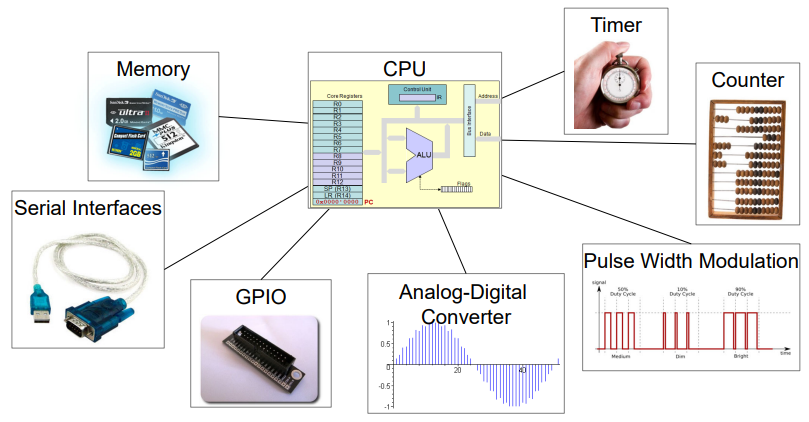
\includegraphics[width=\linewidth]{single_chip_solution.png}

\multend

\subsubsection{Peripherals and Registers}

\begin{definition}{Peripherals}

    \begin{minipage}{0.35\linewidth}
    \begin{itemize}
        \item configurable hardware blocks \\ of a microcontroller
        \item accepts specific task from CPU, \\ executes task and returns result \\ (status, e.g. task completion, error)
        \item often interfaces to outside world\\
        many (not all) interact with \\ external MCU pins 
        \item examples: GPIO, UART, SPI, ADC
    \end{itemize}
    \end{minipage}
    \begin{minipage}{0.64\linewidth}
        \vspace{-5mm}
        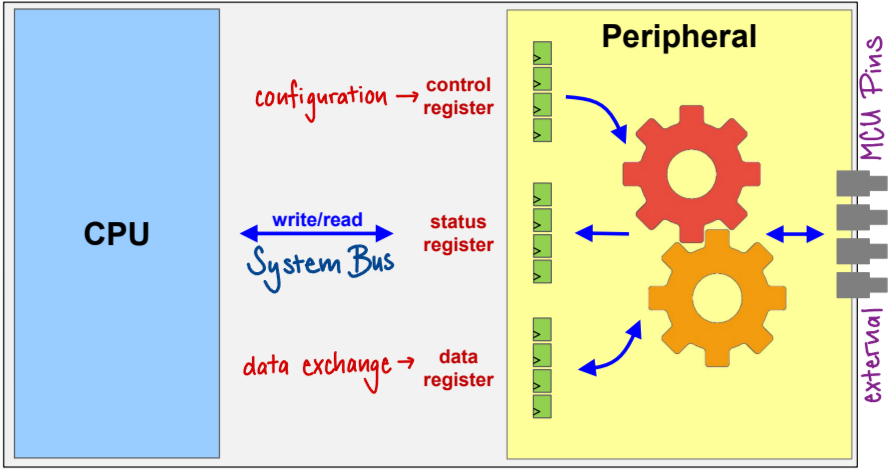
\includegraphics[width=\linewidth]{peripherals_registers.png}
    \end{minipage}
\end{definition}

\mult{2}

\begin{definition}{Registers}
    \begin{itemize}
        \item Registers are arrays of flip-flops (storage elements with two states, i.e. 0 or 1)
        \item Each flip-flop stores one bit of information
        \item CPU writes to and reads from registers
    \end{itemize}
\end{definition}

\begin{theorem}{CPU read/write to peripheral registers}\\
    How does the CPU write to and read from peripheral registers?
    \vspace{-2mm}\\
    \begin{itemize}
        \item CPU reads/writes to peripheral registers
        \item CPU uses memory-mapped I/O to access peripheral registers
        \item CPU uses load/store instructions to access peripheral registers
    \end{itemize}
    $\Rightarrow$ System Buses
\end{theorem}

\begin{concept}{Control and Status Registers}\\
Peripherals interact with the CPU through registers:
\begin{itemize}
    \item \textbf{Control Registers}: CPU configures peripherals
    \begin{itemize}
        \item CPU writes to register bit
        \item Slave hardware uses the output of this bit
        \item Usually read/write
    \end{itemize}
    \item \textbf{Status Registers}: CPU monitors peripheral state
    \begin{itemize}
        \item Slave writes status into register bit
        \item CPU reads register bit
        \item Usually read-only
    \end{itemize}
\end{itemize}
Both control \& status bits can be in same register.
\begin{itemize}
    \item \textbf{Data Registers} \\
        enable CPU to exchange data with the peripheral
\end{itemize}
\end{concept}

\raggedcolumns
\multend

\begin{concept}{CPU access to individual Peripheral Registers}
    \begin{itemize}
        \item ARM \& STM map the peripheral registers into
        the memory address range
        \item Reference Manual shows the defined addresses
    \end{itemize}
    \vspace{2mm}
    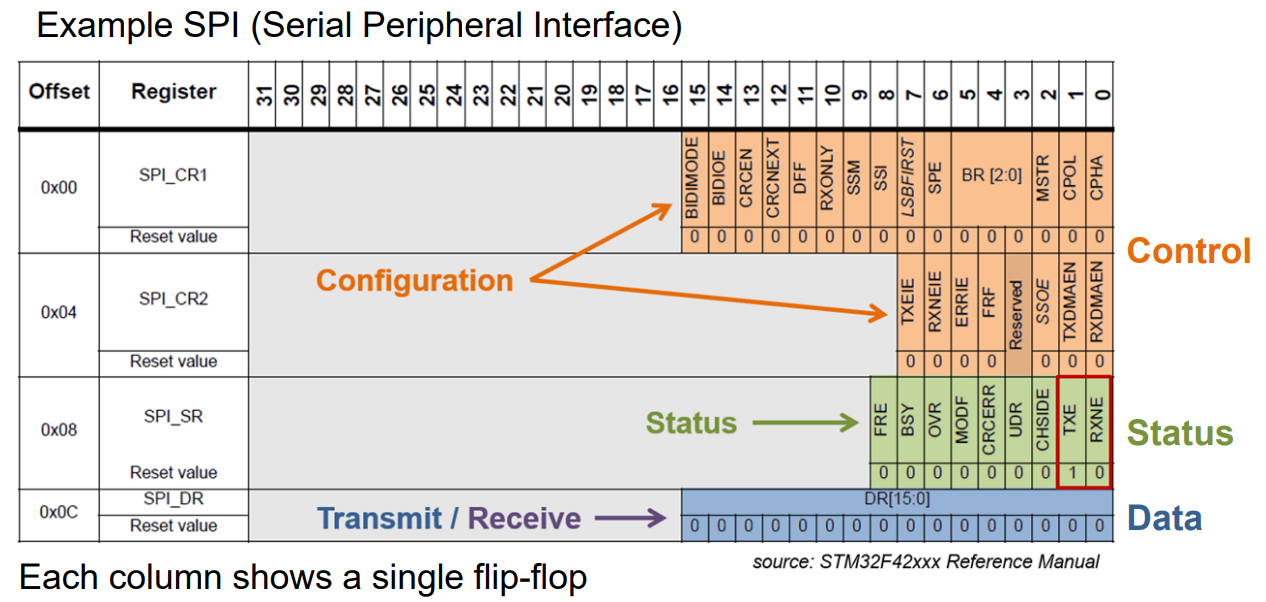
\includegraphics[width=\linewidth]{example_SPI_cpu_access.png}
\end{concept}

\mult{2}

\begin{definition}{Memory mapping of Peripheral Registers}
    \begin{itemize}
        \item Each peripheral register has a unique address
        \item CPU uses the address to access the register
        \item CPU uses load/store instructions to access the register
    \end{itemize}
    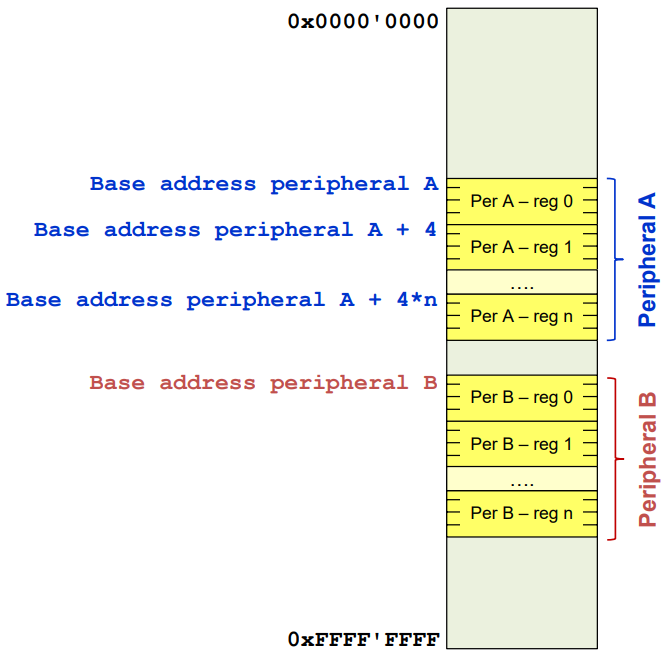
\includegraphics[width=\linewidth]{peripheral_registers_cpu_access.png}
\end{definition}

\begin{definition}{Memory-Mapped Peripheral Registers}
    \begin{itemize}
        \item Control register: controls states of LEDs
        \item Status register: monitors states of DIP switches
    \end{itemize}
    \vspace{1mm}
    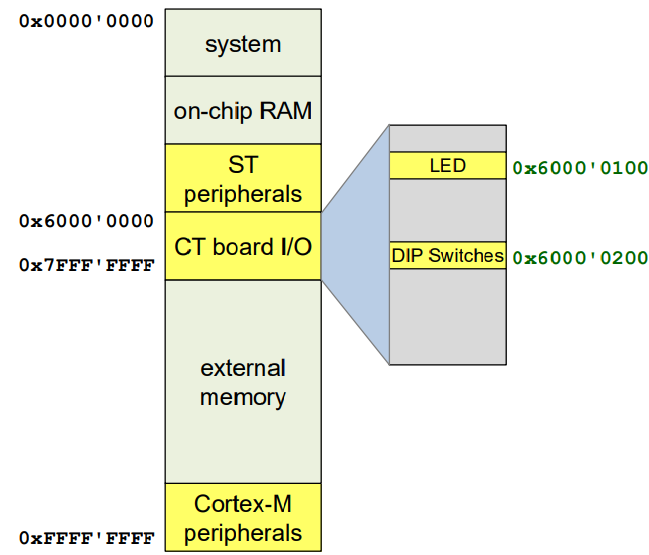
\includegraphics[width=\linewidth]{registers_leds_dipswitches.png}
\end{definition}

\multend

\begin{code}{Memory-Mapped Registers}\\
Registers are mapped into the memory address range - each has a specific address:
\begin{lstlisting}[language=C, style=basesmol]
// Define memory-mapped register addresses
#define ADDR_LED_31_0       0x60000100
#define ADDR_DIP_SWITCH_31_0 0x60000200

// Read from DIP switches and write to LEDs
uint32_t value = read_word(ADDR_DIP_SWITCH_31_0);
write_word(ADDR_LED_31_0, value);
\end{lstlisting}
\end{code}


\subsubsection{System Bus}
\mult{2}


\begin{definition}{System Bus}
    \begin{itemize}
        \item Interconnects CPU with memory and peripherals, \\allowing data transfer between components.
        \item CPU acts as master: initiating and controlling all transfers
        \item Peripherals and memory act as slaves: responding to requests from the CPU
        \item System bus is a shared resource
    \end{itemize}
    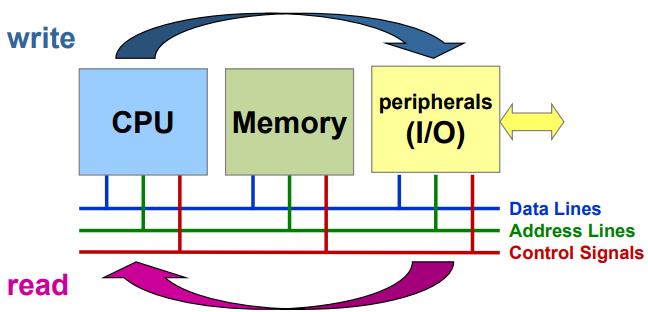
\includegraphics[width=\linewidth]{system_bus.png}\\
    The CPU acts as a master, initiating and controlling all transfers, while peripherals and memory act as slaves, responding to requests.
\end{definition}



\begin{theorem}{Signal Groups}
    \begin{itemize}
        \item \textcolor{darkblue}{\textbf{Data lines}}
        \begin{itemize}
            \item Bidirectional (read/write)
            \item Number of lines $\rightarrow$ data bus width \\(8, 16, 32, 64 parallel lines of data)
            \item Example: Cortex-M has 32 address lines $\rightarrow$ 4GB address space \\ $\rightarrow$ \texttt{0x00000000} to \texttt{0xFFFFFFFF}
        \end{itemize}
        \item \textcolor{darkgreen}{\textbf{Address lines}}
        \begin{itemize}
            \item Unidirectional: from Master to slaves
            \item Number of lines $\rightarrow$ size of address space \\ (e.g., 32 lines allow $2^{32}$ addresses)
        \end{itemize}
        \item \textcolor{darkred}{\textbf{Control signals}}
        \begin{itemize}
            \item Control read/write direction
            \item Provide timing information
            \item Chip select, read/write, etc.
        \end{itemize}
    \end{itemize}
    \vspace{2mm}
    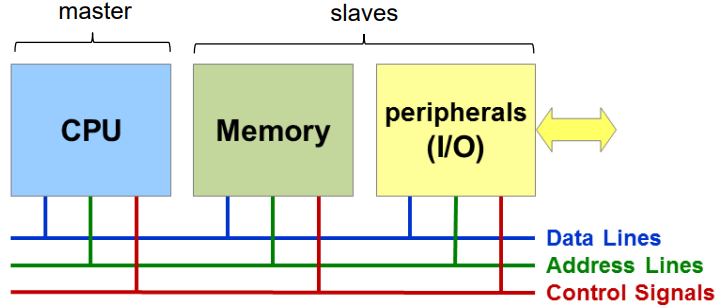
\includegraphics[width=\linewidth]{master_slave_signal_groups.png}
\end{theorem}

\begin{concept}{Bus Specification}
    \begin{itemize}
        \item \textcolor{darkblue}{\textbf{Protocol and operations}}
        \item \textcolor{darkred}{\textbf{Signals}}
        \begin{itemize}
            \item Number of Signals
            \item Signal descriptions
        \end{itemize}
        \item \textcolor{darkgreen}{\textbf{Timing}}
        \begin{itemize}
            \item Frequency
            \item Setup and hold times
        \end{itemize}
        \item \textcolor{darkpurple}{\textbf{Electrical properties}} (not in exam)
        \begin{itemize}
            \item Drive strength and Load
        \end{itemize}
        \item \textcolor{darkorange}{\textbf{Mechanical requirements}} (not in exam)
    \end{itemize}
\end{concept}

\columnbreak

\begin{theorem}{Bus Timing Options}\\
    \textbf{Synchronous}
    \begin{itemize}
        \item \textcolor{blue}{Master} and \textcolor{darkcorn}{slaves} use a common clock\\
        Often dedicated CLK signal from master to slave, \\ but clock can also be encoded in a data signal
        \item Clock edges control bus transfer on both sides
        \item Used by most on-chip buses
        \item Off-chip: DDR and synchronous RAM
    \end{itemize}
    \begin{center}
    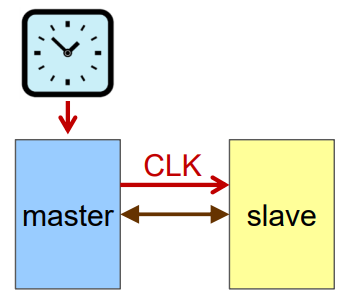
\includegraphics[width=0.6\linewidth]{synchronous_bus_timing.png}
    \end{center}
    \textbf{Asynchronous}
    \begin{itemize}
        \item \textcolor{darkcorn}{Slaves} have no access to clock of the \textcolor{blue}{master}
        \\ $\rightarrow$ slave has their own clock or no clock at all
        \item Control signals carry timing information to allow synchronization
        \item Widely used for low data-rate off-chip memories \\
        $\rightarrow$ parallel flash memories and asynchronous RAM
    \end{itemize}
    \begin{center}
        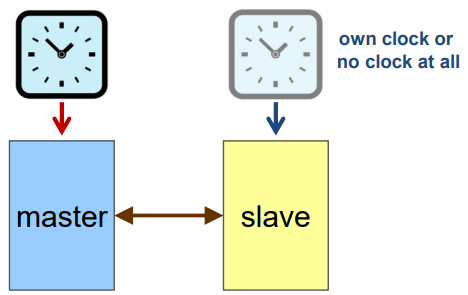
\includegraphics[width=0.6\linewidth]{asynchronous_bus_timing.png}
    \end{center}
\end{theorem}

\important{But how can a driver be disconnected electrically?}

\begin{corollary}{Multiple devices driving the same data line}\\
    What if one device drives a logic 1 (Vcc) and another device drives a logic 0 (Gnd)?\\
    $\Rightarrow$ Electrical short circuit!
    \\ $\rightarrow$ bus contention ('Streitigkeit')\\
    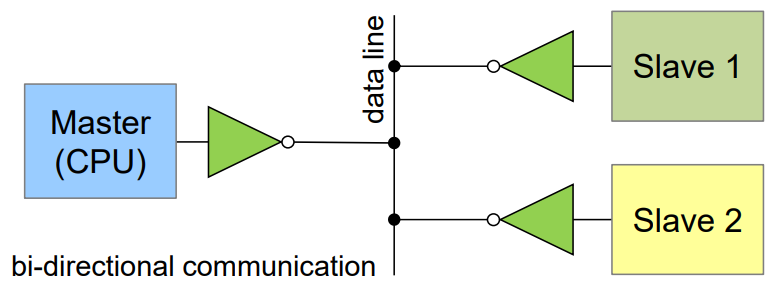
\includegraphics[width=\linewidth]{bus_contention.png}\\
    \small{Figure only shows output paths, input paths are not shown.}

\end{corollary}



\multend


\subsection{Digital Logic Basics}

\mult{2}

\begin{definition}{CMOS Inverter}
    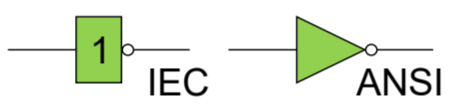
\includegraphics[width=0.5\linewidth]{cmos_inverter0.png}\\
    Complementary switches (transistors)\\
    $\rightarrow$ \textcolor{red}{p-type} and \textcolor{blue}{n-type} have opposite open-close behaviour\\
    \\
    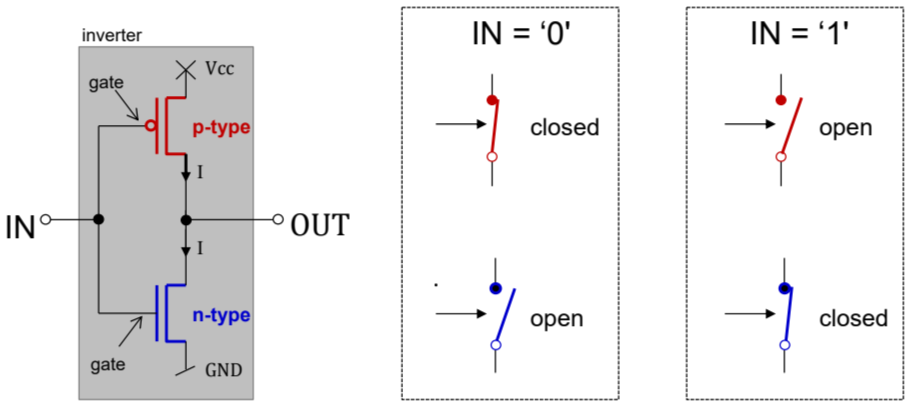
\includegraphics[width=\linewidth]{cmos_inverter1.png}\\
    e.g. Vcc = 3V = '1', Gnd = 0V = '0'\\
    Vcc is the supply voltage of the circuit/chip
    \vspace{2mm}\\
    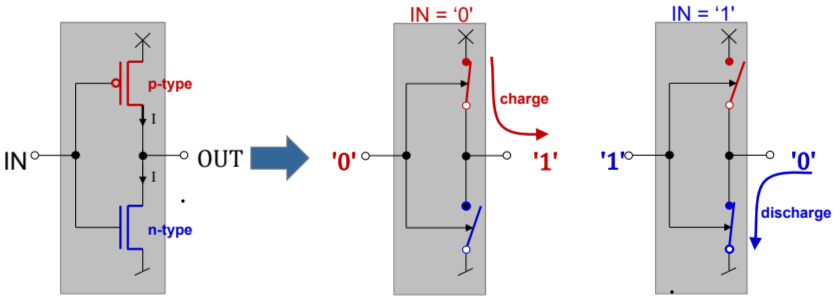
\includegraphics[width=\linewidth]{cmos_inverter2.png}\\
    A buffer is built by connecting two inverters in series
\end{definition}

\begin{definition}{CMOS Tri-State Inverter}\\
    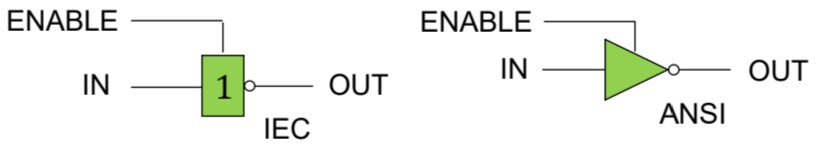
\includegraphics[width=\linewidth]{tristate_inverter1.png}\\
    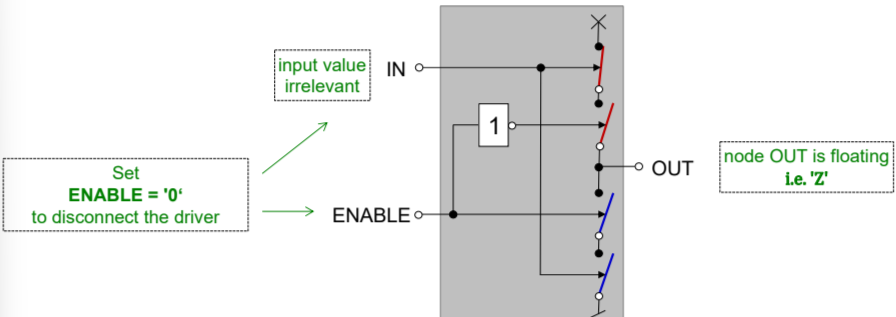
\includegraphics[width=\linewidth]{tristate_inverter3.png}\\
    Implementation:\\
    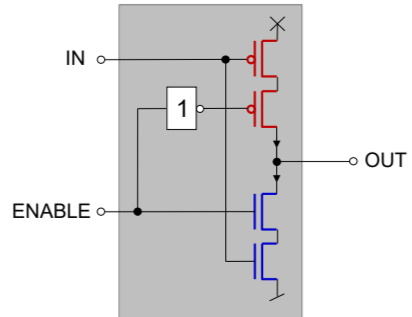
\includegraphics[width=\linewidth]{tristate_inverter4.png}
\end{definition}

\begin{definition}{Tri-State Logic}\\
Multiple devices can drive the same data line thanks to tri-state capability:
\begin{itemize}
    \item Logic '1': Voltage level (e.g., 3.3V)
    \item Logic '0': Ground (0V)
    \item Third state 'Z': High impedance (disconnected, floating)
\end{itemize}
The CPU defines which device drives the bus:
\begin{itemize}
    \item \textbf{Write}: CPU drives bus, all slave drivers disconnected
    \item \textbf{Read}: CPU driver disconnected, selected slave drives bus, other slave drivers disconnected
\end{itemize}
\end{definition}


\begin{concept}{Tri-State Buffer} Timing Diagram\\
    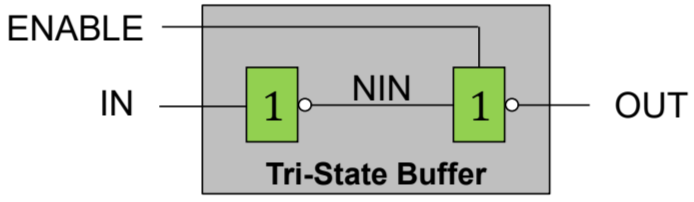
\includegraphics[width=\linewidth]{tristate_buffer1.png}\\
    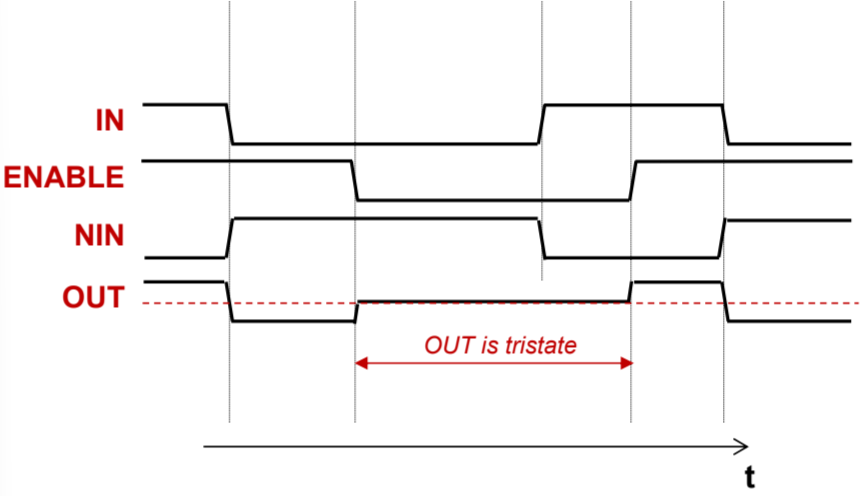
\includegraphics[width=\linewidth]{tristatebuffer2.png}\\
    When a signal like OUT is in tristate, we often say that it is 'floating'. 
    The term expresses that such a signal can easily be moved by parasitic electrical effects
    to either one of the reference levels, i.e. '0' or '1'.
\end{concept}

\begin{KR}{Bus Contention} \\
    CPU defines who drives the data bus at which moment in time:
    \begin{itemize}
        \item \texttt{write} CPU drives bus $\rightarrow$ all slave drivers disconnected
        \item \texttt{read} CPU releases bus $\rightarrow$ one slave drives bus (selected through values on address lines, other slave drivers disconnected)
    \end{itemize}
    
    Electrically disconnecting a driver is called \textbf{tri-state} or \textbf{high-impedance} (Hi-Z) state. (switch)
    
    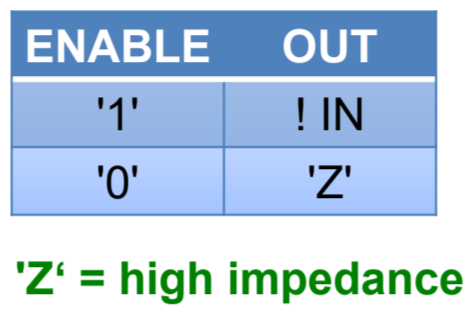
\includegraphics[width=0.5\linewidth]{tristate_inverter2.png}\\
\end{KR}



\multend

\subsection{Synchronous Bus}

\mult{2}

\begin{definition}{Synchronous Bus}\\
    Example Uses External Bus from ST Microelectronics
    \begin{itemize}
        \item Reason: Internal workings of the system bus are not disclosed by STM
        \item Signal names, bus protocol and timing based on external synchronous STM32F429xx mode instead
        \item For details see Chapter 37, Flexible memory controller (FMC) in ST Reference Manual RM0090
        \item Datasheet STM32F429xx
        \item Figure 60 Synchronous non-multiplexed NOR/PSRAM read timings
        \item Figure 61 Synchronous non-multiplexed PSRAM write timings
    \end{itemize}
Naming Convention
\begin{itemize}
    \item Letter ' N ' prefix in signal name ( $\mathrm{N} x x x$ ) means active-low signal
    \item E.g. NOE means 'NOT OUTPUT ENABLE'
\end{itemize}

NOE $=$ ' 0 ' $\rightarrow$ output enabled\\
NOE $=$ ' 1 ' $\rightarrow$ output disabled
\end{definition}

\begin{concept}{Synchronous Bus Timing}\\
Key signals for read/write operation:
\begin{itemize}
    \item \textbf{CLK}: System clock
    \item \textbf{A[31:0]}: Address lines
    \item \textbf{D[31:0]}: Data lines
    \item \textbf{NWE}: Not Write Enable (active low)
    \item \textbf{NOE}: Not Output Enable (active low)
    \item \textbf{NE}: Not Enable (active low)
\end{itemize}
Note that 'N' prefix indicates active-low signals.
\end{concept}



\begin{formula}{Block Diagram}\\
    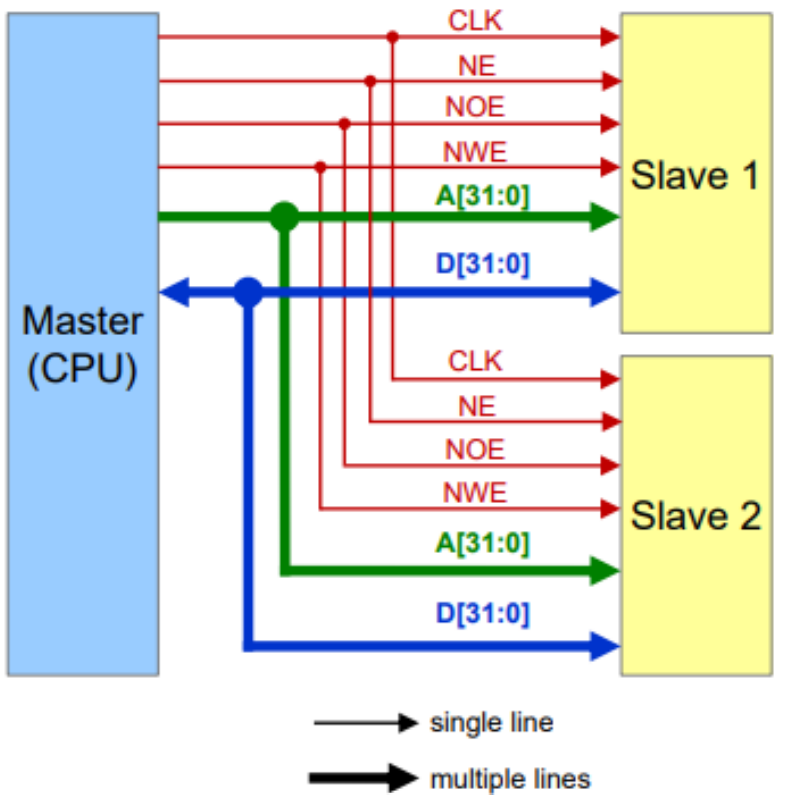
\includegraphics[width=\linewidth]{block_diagramm.png}
\end{formula}

\begin{definition}{Bus Timing Diagram}
    \begin{itemize}
        \item CLK $\rightarrow$ clock signal (rising edge)
        \item NE $\rightarrow$ Not enable (active low)
        \item NWE $\rightarrow$ Not write enable (active low)
        \item NOE $\rightarrow$ Not output enable (active low)
    \end{itemize}
    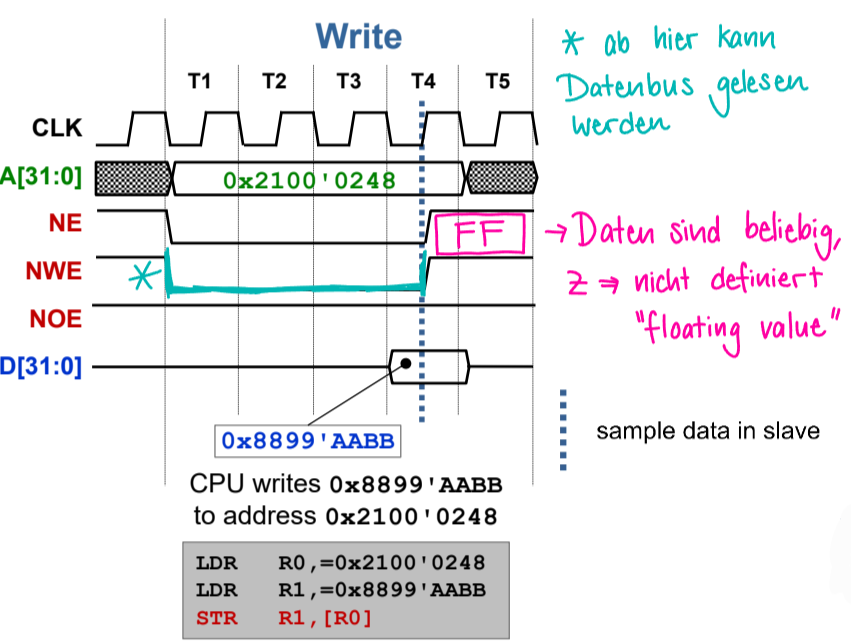
\includegraphics[width=\linewidth]{timing_diagram1.png}

    \begin{minipage}{0.4\linewidth}
        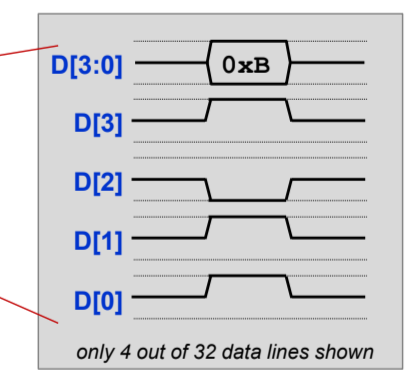
\includegraphics[width=\linewidth]{timing2.png}
    \end{minipage}
    \begin{minipage}{0.54\linewidth}
        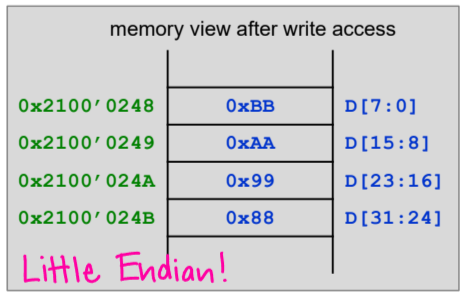
\includegraphics[width=\linewidth]{timing3.png}
    \end{minipage}
    \vspace{1mm}\\
    WICHTIG: nicht genau mit Flanke schreiben, Daten brauchen eine gewisse Zeit um stabil zu werden (keine genaue Definition, muss einfach 'genug' sein)\\
    READ dauert länger als WRITE, da die Daten erst stabil werden müssen bevor sie gelesen werden können
\end{definition}

\begin{theorem}{Bus Timing Diagrams}\\ Notation for Groups of Signals\\
    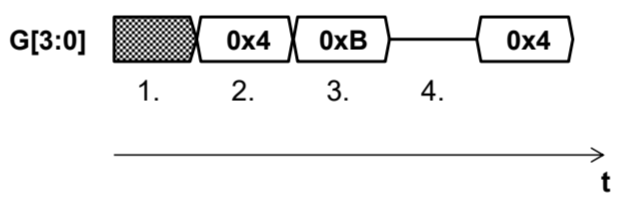
\includegraphics[width=\linewidth]{bus_timing_notation.png}\\
    Group G of 4 signals

1. unknown values

The values on each of the 4 signals are either ' 1 ' or ' 0 ', but unknown.

2. The bus holds the value $0 \times 4$
$$
\text { i.e. } \mathrm{G}[3]=\text { ' } 0 \text { ', G[2] = '1', G[1] = '0', G[0] = '0' }
$$
3. The bus holds the value $0 \times B$
$$
\text { i.e. } \mathrm{G}[3]=\text { ' } 1 \text { ', G[2] = '0', G[1] = '1', G[0] = '1' }
$$
4. Tri-state

All signals $\mathrm{G}[3: 0$ ] are tri-state (i.e. ' $Z$ ' or high-impedance). "No one is driving the bus"
\end{theorem}

\multend



\begin{formula}{Timing Diagram}  
    \begin{itemize}
        \item \texttt{write} \textcolor{darkblue}{D[:]} to \textcolor{darkgreen}{A[:]} $\rightarrow$ \textcolor{darkred}{NE, NWE} = 0
        \item \texttt{read} \textcolor{darkblue}{D[:]} from \textcolor{darkgreen}{A[:]} $\rightarrow$ \textcolor{darkred}{NE, NOE} = 0
    \end{itemize}
    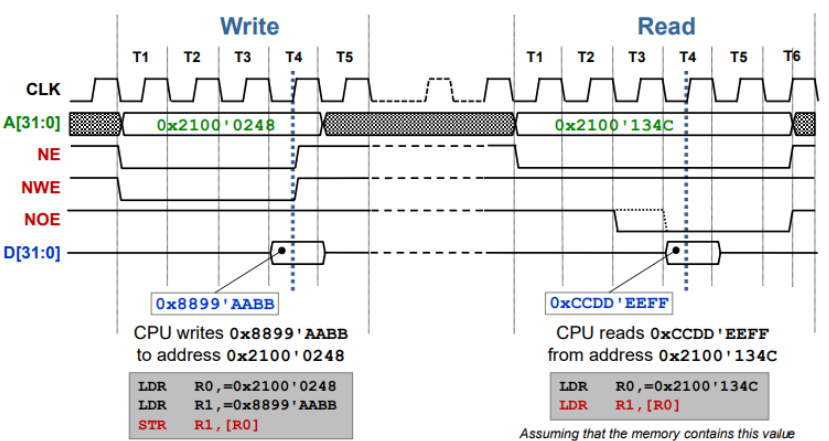
\includegraphics[width=\linewidth]{timing_diagram.png}
\end{formula}




\begin{theorem}{Bus Access Size}
    is determined by the NBL (0-3) (No Byte Line) signals
    \begin{itemize}
        \item NBL = 1 $\rightarrow$ Byte used for Read/Write
        \item NBL = 00
        \item NBL[0:3] = 0011 $\rightarrow$ Read Halfword
        \item NBL[0:3] = 1111 $\rightarrow$ Read Word
    \end{itemize}
    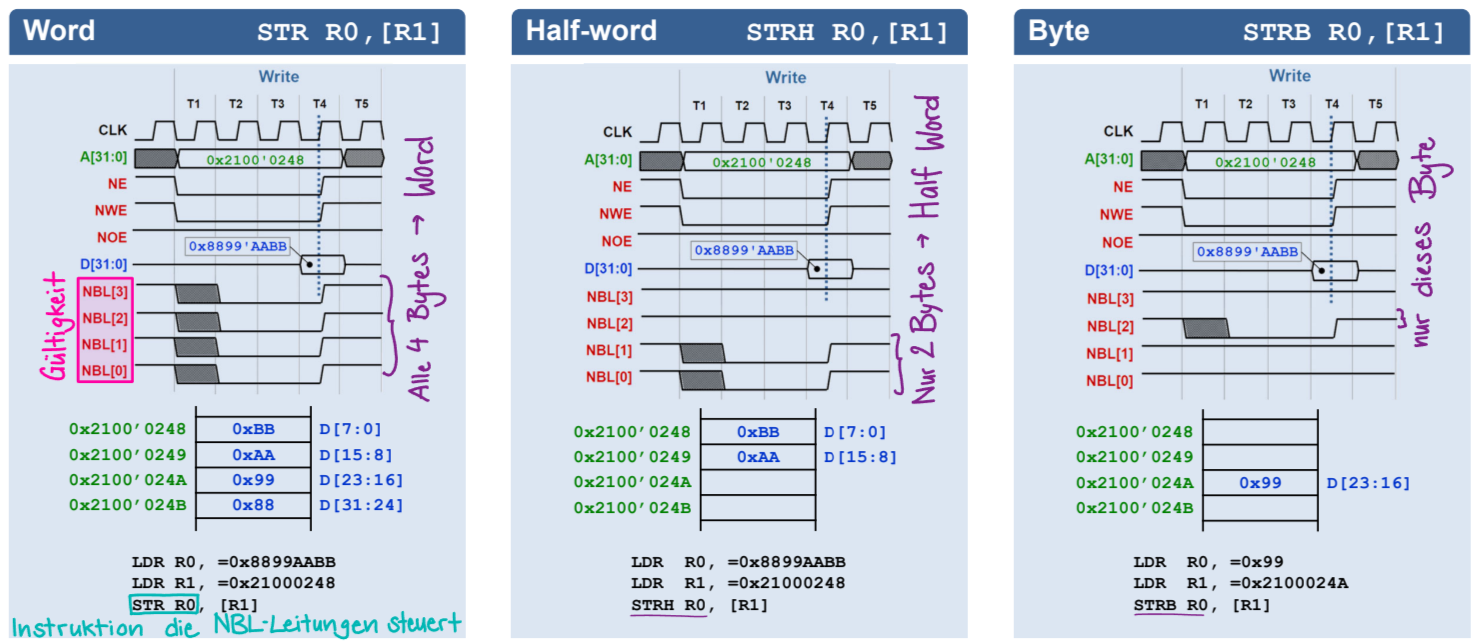
\includegraphics[width=\linewidth]{bus_access_size.png}\\
    Gültigkeit: damit zeigt die CPU an, welche der 4 Bytes übertragen werden sollen (gültig = 0 (unten))\\
    \begin{itemize}
        \item Exact Position of falling edge on NBL varies with chip version
        \item Value on unused data lines are unknown, figues show assumptions
    \end{itemize}
\end{theorem}


\subsection{Control and Status Registers}

\begin{definition}{Hardware Slave (Peripheral)}\\
    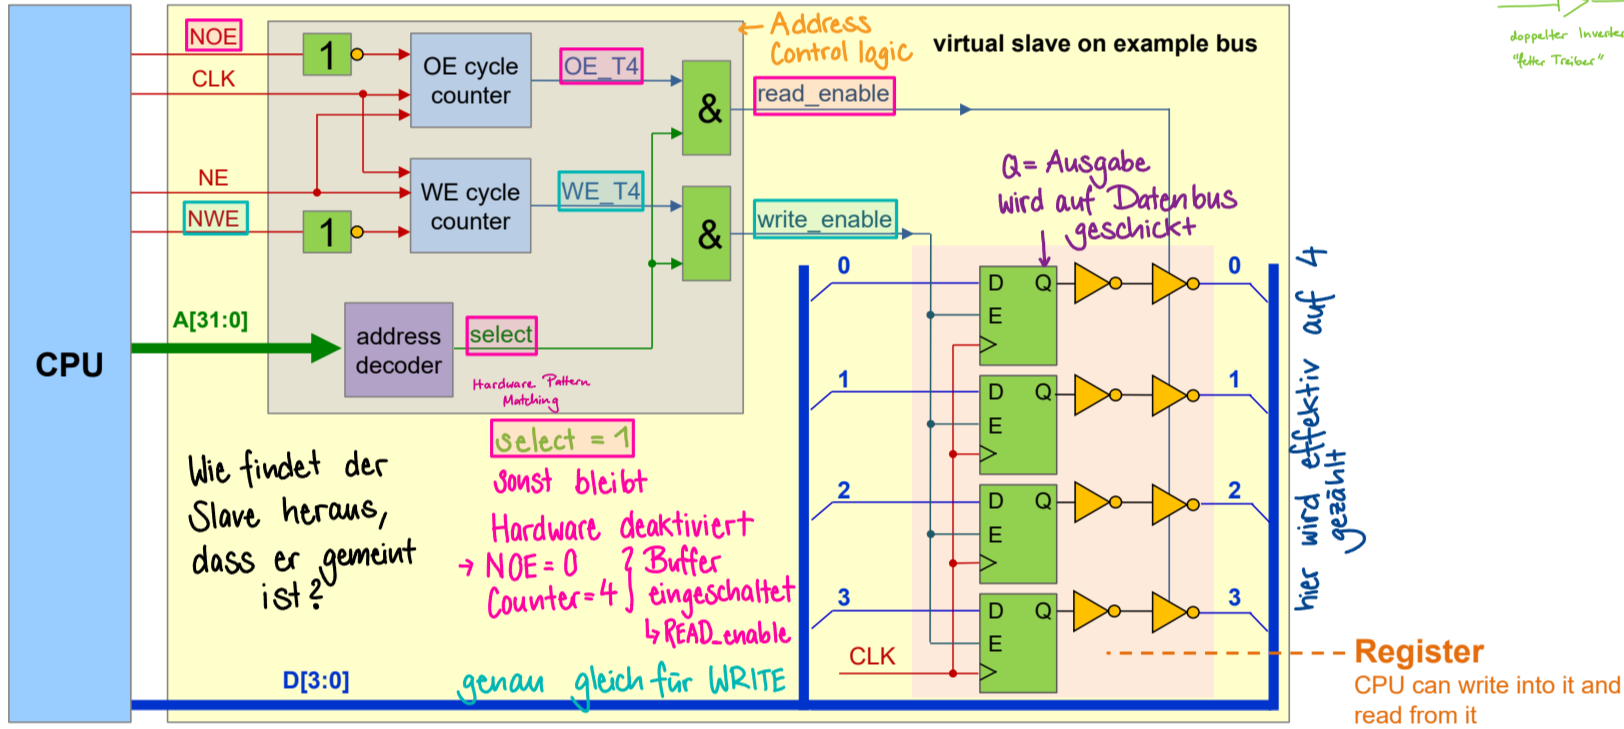
\includegraphics[width=\linewidth]{hardware_slave.png}
\end{definition}

\mult{2}

\begin{concept}{Control Bits}
    \begin{itemize}
        \item Allow CPU to configure Slaves
        \item CPU writes to register bit to configure Slave
        \item Slave uses output of register bit to configure itself
        \item Example: SPI Slave Select (SS) bit
        \item Usually read/write access to control bits
    \end{itemize}
\end{concept}

\begin{concept}{Status Bits}
    \begin{itemize}
        \item Allow CPU to monitor Slaves
        \item CPU reads register bit to monitor Slave
        \item Slave uses input of register bit to monitor itself (Slave writes to register bit)
        \item Example: SPI Busy bit
        \item Usually read-only access to status bits
    \end{itemize}
\end{concept}

\multend

\begin{example}
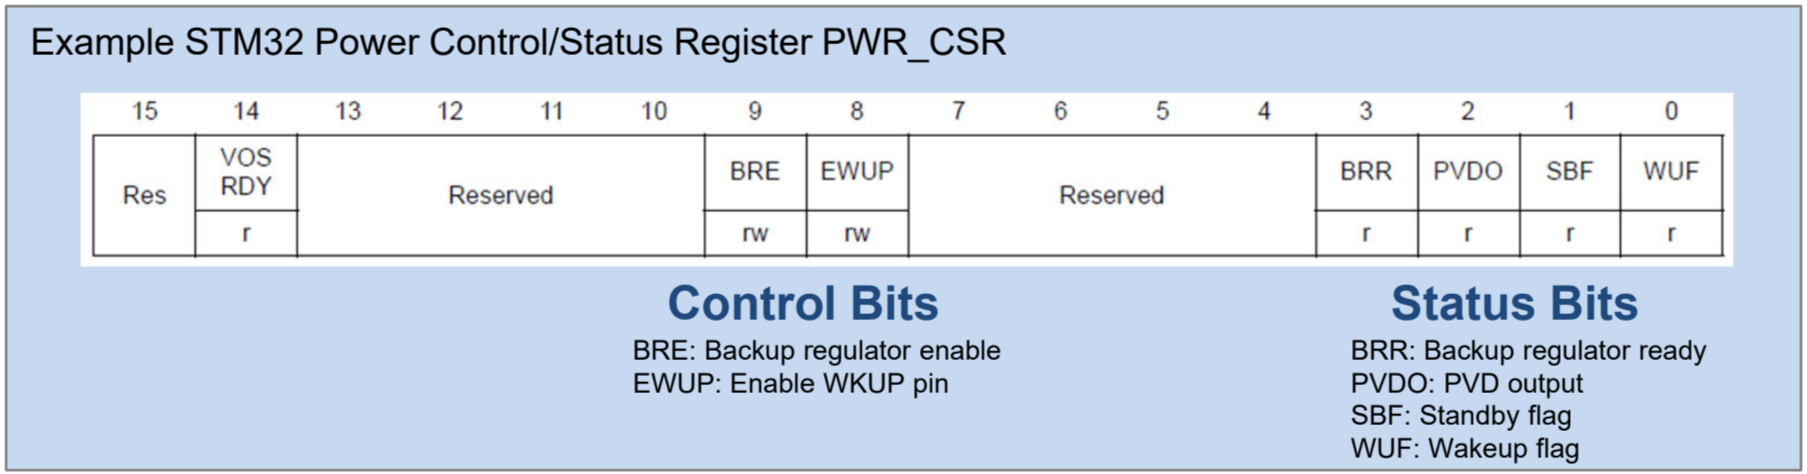
\includegraphics[width=\linewidth]{example_control_status_regs.png}\\
Control/Status register on example bus:

\begin{minipage}{0.5\linewidth}
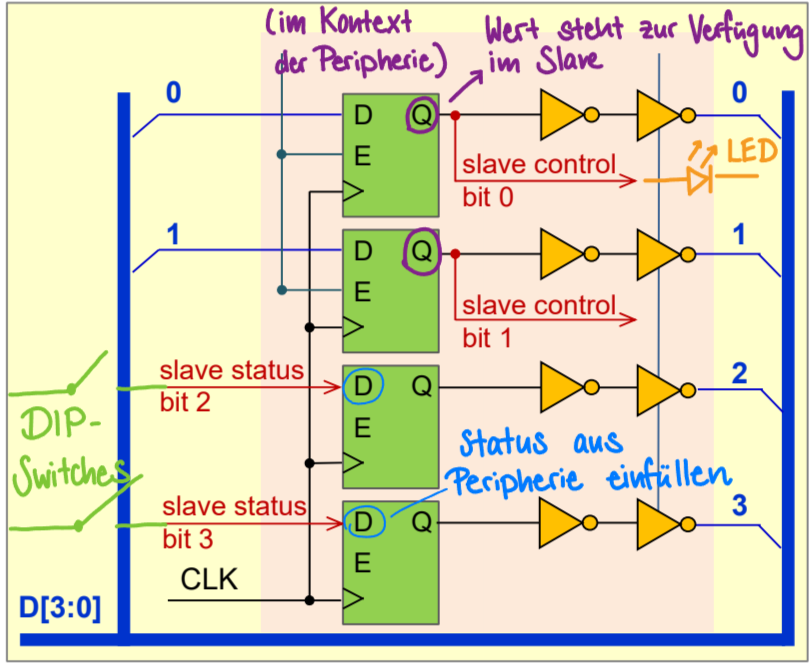
\includegraphics[width=\linewidth]{example_control_status_regs2.png}
\end{minipage}
\begin{minipage}{0.4\linewidth}
control bits: 0 and 1\\
status bits: 2 and 3\\
The same register may contain both control and status bits!
\end{minipage}
\end{example}

\begin{theorem}{Control and Status Registers on CT Board}\\
    Chip-internal and external registers (details on memory map in STM32 Reference Manual)

    \begin{minipage}{0.4\linewidth}
    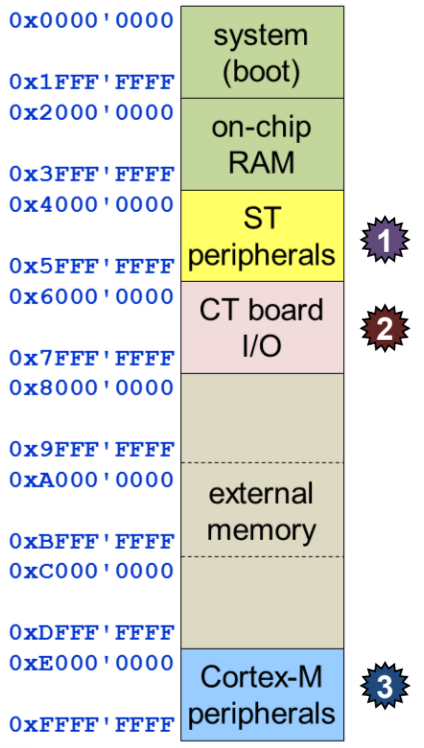
\includegraphics[width=\linewidth]{control_status_regs_ctboard1.png}
    \end{minipage}
    \begin{minipage}{0.54\linewidth}
    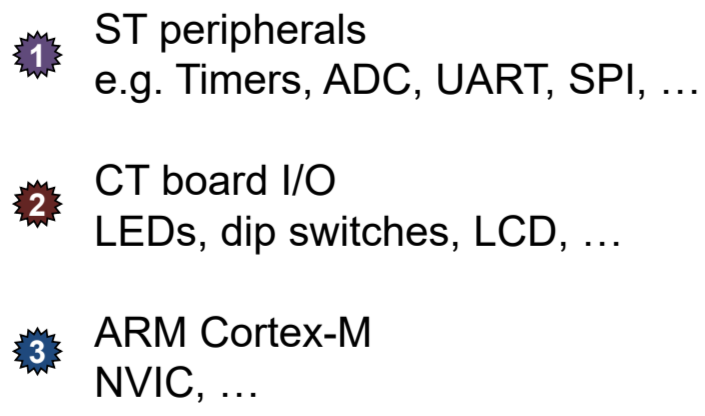
\includegraphics[width=\linewidth]{control_status_regs_ctboard2.png}
    \end{minipage}

    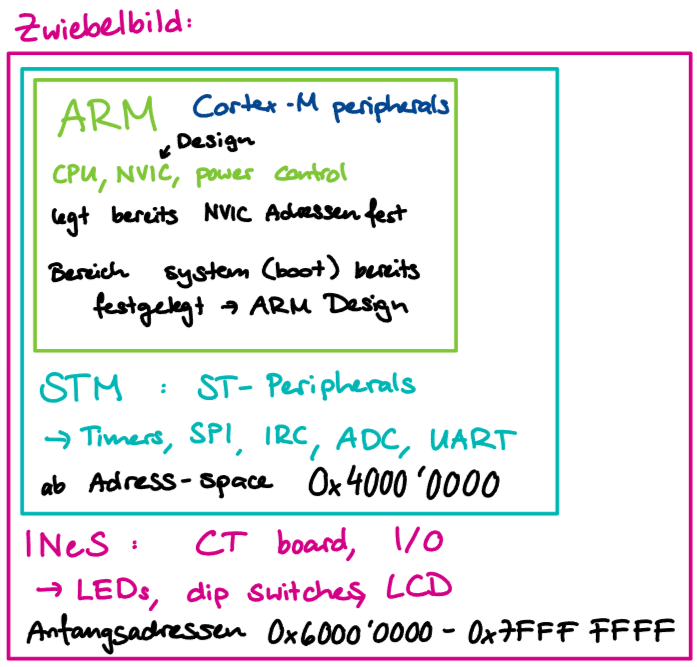
\includegraphics[width=0.6\linewidth]{control_status_regs_ctboard3.png}
\end{theorem}


\subsection{Address Decoding}

\begin{definition}{Address Decoding}\\
    Interpretation of address line values. See whether bus access targets a particular address or address range.
    \begin{itemize}
        \item CPU uses address lines to select a peripheral
        \item Each peripheral has a unique address range
        \item Address decoding logic generates a chip select signal for each peripheral
    \end{itemize}

    \textbf{Full Address Decoding}
    \begin{itemize}
        \item All address lines are decoded
        \item A control register can be accessed at exactly one location
        \item 1:1 mapping: A unique address maps to a single hardware register
        \item example: LEDs and DIP switches on CT board
    \end{itemize}

    \textbf{Partial Address Decoding}
    \begin{itemize}
        \item Only a subset of address lines are decoded
        \item A control register can be accessed at multiple locations
        \item 1:n mapping: Multiple addresses map to the same hardware register
        \item Motivation: Simpler and possible Aliasing (Map a hardware register to several addresses)
    \end{itemize}
    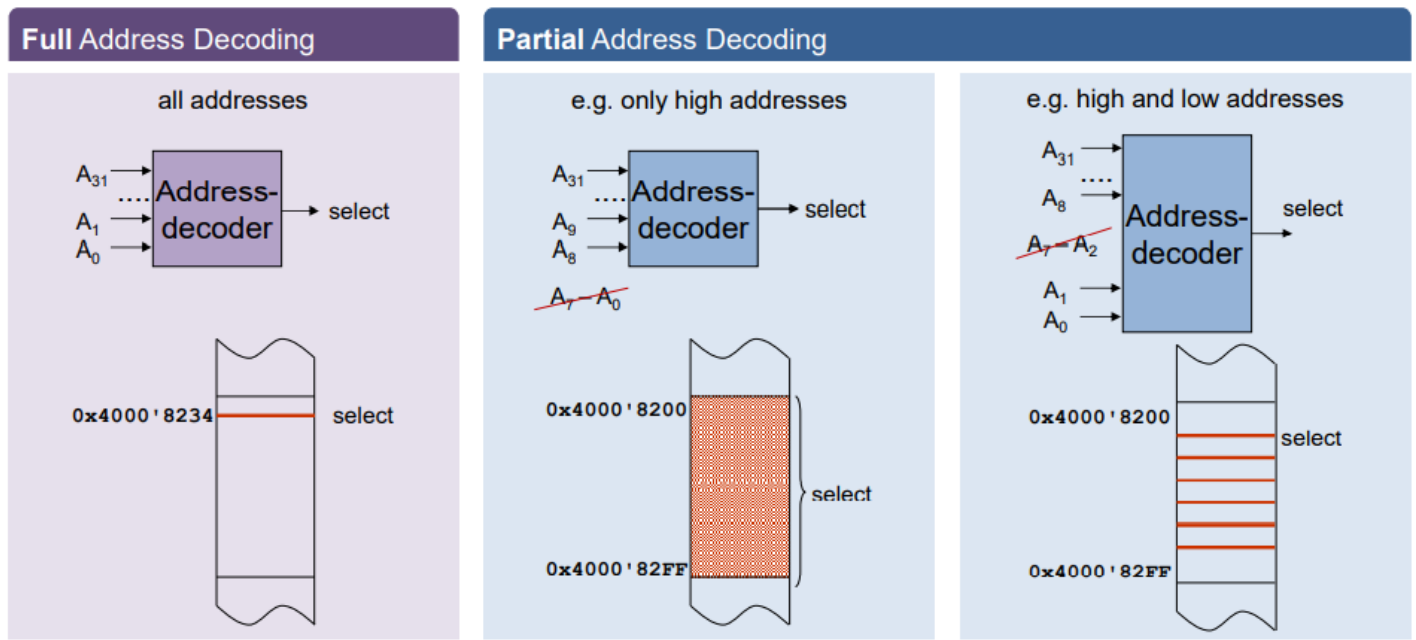
\includegraphics[width=\linewidth]{address_decoding.png}
\end{definition}

\begin{examplecode}{Simple Address Decoder}\\
Basic address decoder with 3 address lines that selects when address is 0x5:
\begin{lstlisting}[language=C, style=basesmol]
// In hardware description language (e.g., Verilog):
assign select = (A[2] & !A[1] & A[0]); // Decodes address 0x5 (101 binary)
\end{lstlisting}
\end{examplecode}

\begin{example2}{Address Decoding Exercise}\\
Given a system bus with 6 address lines A[5:0], determine the address ranges if only bits A[5:4] are decoded.
\tcblower
This means the lower 4 bits (A[3:0]) are not decoded, resulting in a partial address decoding.

Each decoded address represents a range of $2^4 = 16$ addresses.

If A[5:4] = 01, the corresponding address range is:
- Start: 0x10 (binary: 010000)
- End: 0x1F (binary: 011111)

All addresses in this range (0x10 through 0x1F) will select the same device.
\end{example2}

\columnbreak

\begin{theorem}{Address Range Calculation}\\
For partial address decoding, if only higher-order address bits \(A[n:m]\) are decoded (where \(n > m\)), then:
\begin{itemize}
    \item Each decoded address represents a range of \(2^m\) addresses
    \item The size of this address range is \(2^m\) bytes
    \item The start address has all lower bits set to 0
    \item The end address has all lower bits set to 1
\end{itemize}
For example, if only \(A[31:8]\) are decoded, each decoded address represents a 256-byte range (\(2^8 = 256\)).
\end{theorem}

\begin{remark}
    How does a Slave know that it is being addressed?\\
    $\Rightarrow$ Address decoding logic in the Slave (each on its own)
\end{remark}



\begin{example}
    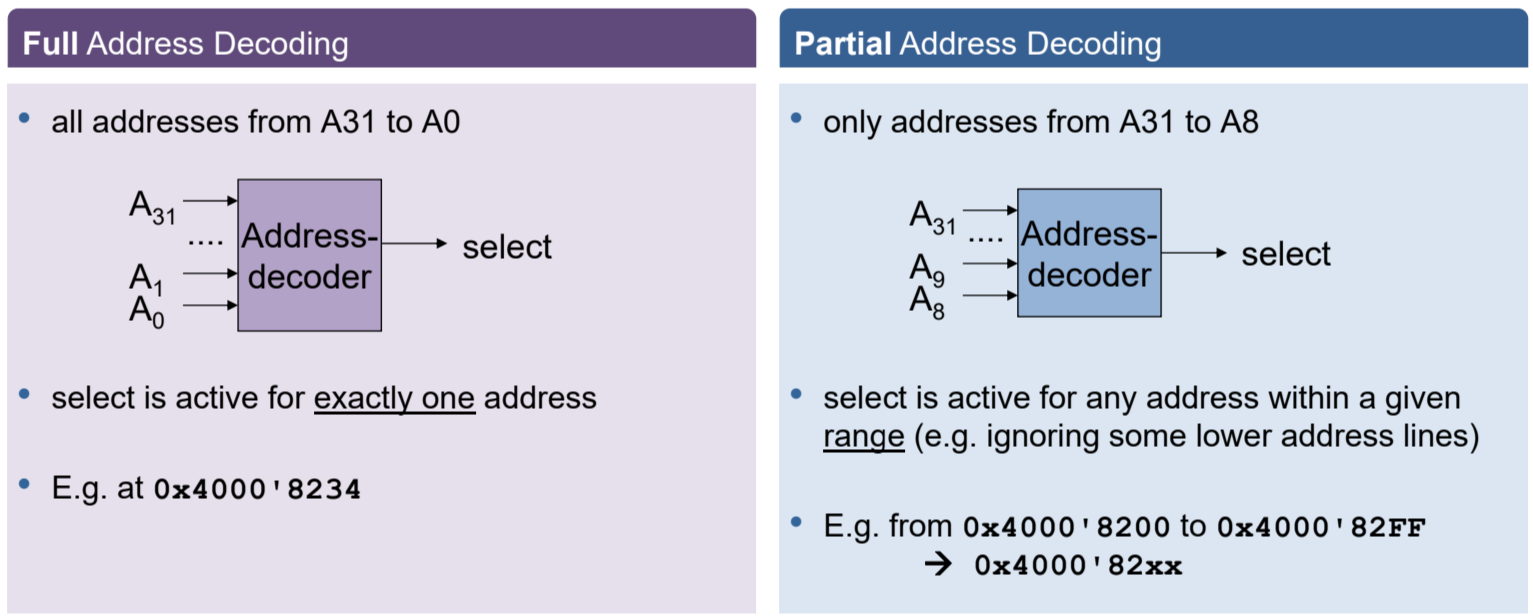
\includegraphics[width=\linewidth]{example_address_decoding.png}\\
    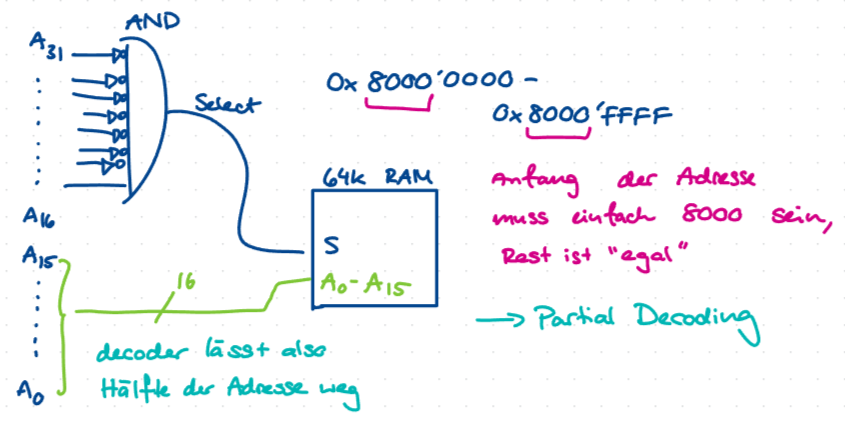
\includegraphics[width=\linewidth]{example_address_decoding2.png}
\end{example}



\columnbreak

\subsection{Wait States for Slow Peripherals}

\begin{definition}{Wait States}\\
Wait states are extra clock cycles inserted to allow slow peripherals to respond.
\begin{itemize}
    \item Without wait states, the slowest slave would determine bus cycle time
    \item Wait states can be:
    \begin{itemize}
        \item Programmed at a bus interface unit depending on the address
        \item Requested by slaves through a "ready" signal (for long or variable access times)
    \end{itemize}
\end{itemize}
\end{definition}

\begin{definition}{Slow Slaves}\\
    Problem: Individual Slave Access times
    \begin{itemize}
        \item If slowest slave defines bus cycle time $\rightarrow$ reduced bus performance
        \item How can we get an individual bus cycle time for each slave?
    \end{itemize}   
\end{definition}

\begin{concept}{Solutions for slow slaves} two possibilities:
    \begin{itemize}
        \item \textbf{Individual Wait States} can be programmed at a bus interface unit \\
        Insert wait states to slow down the CPU to match the speed of the slowest peripheral (depending on the address of an access/bus cycle)\\
        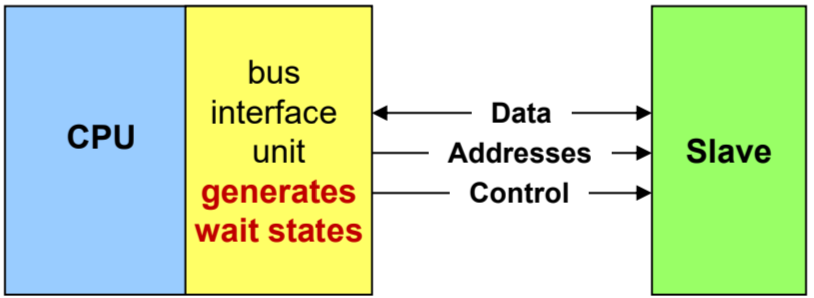
\includegraphics[width=\linewidth]{individual_wait_states.png}
        \item \textbf{Bus Mastering} Slave tells bus interface unit when it is ready \\
        Allow a peripheral to take control of the bus and perform its own accesses (e.g. DMA)\\
        Well suited for slaves with long or variable access times\\
        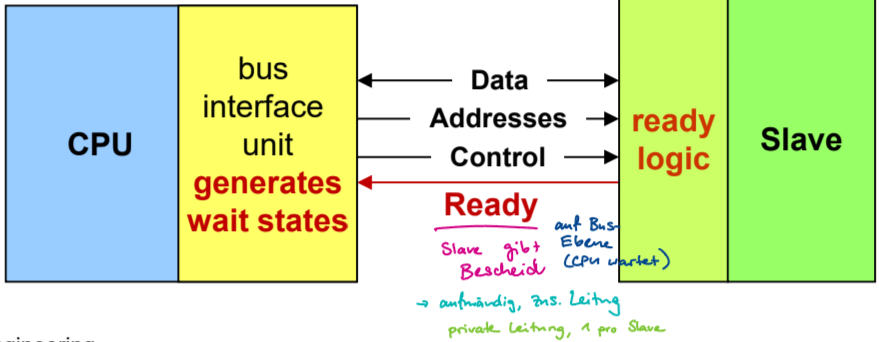
\includegraphics[width=\linewidth]{solution_for_slow_slaves.png}
    \end{itemize}
\end{concept}

\begin{KR}{Individual Wait States}\\
    Wait states are inserted to slow down the CPU to match the speed of the slowest peripheral (depending on the address of an access)

    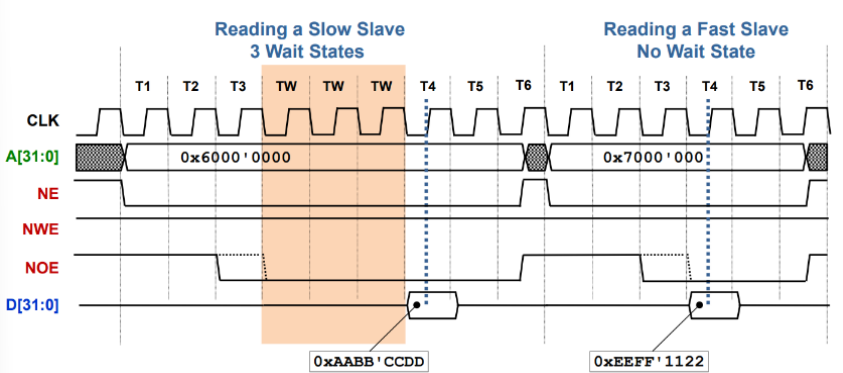
\includegraphics[width=\linewidth]{slow_slaves.png}    
\end{KR}

\subsubsection{Bus Hierarchies}

\begin{example2}{STM32 Microcontroller}\\
    with CPU, on-chip memory, and peripherals interconnected through the system bus(es)
    \begin{itemize}
        \item On-chip system bus: 32 data lines, 32 address lines and control signals
        \item Off-chip external bus: 16 data lines, 24 address lines and control signals
    \end{itemize}
    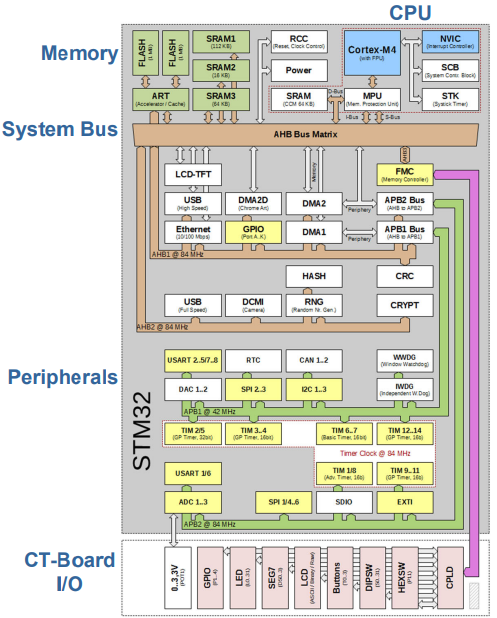
\includegraphics[width=0.9\linewidth]{stm32_example.png}

    A distributed system with parallel (simultaneous) processing of data in many peripherals. All under the supervision of the CPU.
\end{example2}

\begin{remark}
    Note: ARM calls their system buses AHB (ARM High-performance Bus) and APB (ARM
    Peripheral Bus). On complex chips, it is state-of-the-art to partition the system bus into
    multiple interconnected buses.
\end{remark}

\begin{example2}{CT Board with STM32 Microcontroller and Buses}\\
    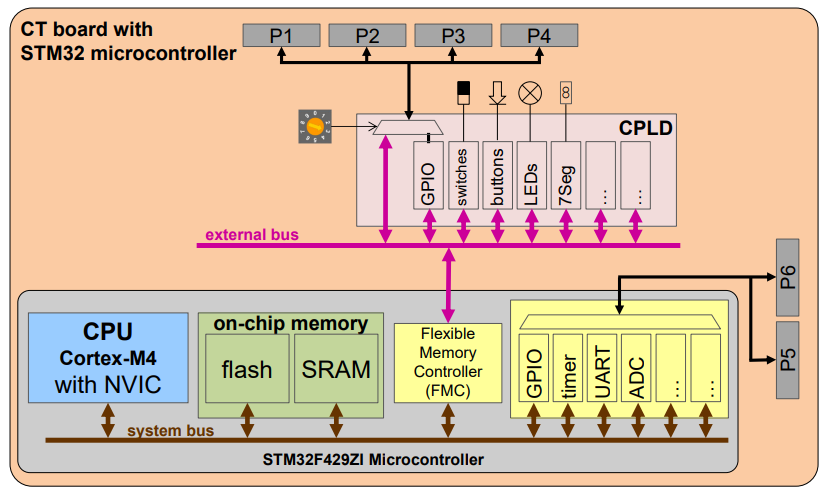
\includegraphics[width=\linewidth]{ctboard_with_stm32.png}\\
    Real-world Systems are partitioned into multiple buses.
\end{example2}

\columnbreak

\subsection{Programming Memory-Mapped Peripherals}

\subsubsection{Accessing Control Registers in C}

\mult{2}

\begin{definition}{Accessing Control Registers in C}\\
    \textbf{Hardware View}
    \begin{itemize}
        \item Signals
        \item Timing
        \item Address decoding
        \item Wait states
        \item Control and status registers
    \end{itemize}
    \textbf{Software View}
    \begin{itemize}
        \item Accessing control and status registers in C
    \end{itemize}
\end{definition}

\begin{concept}{Accessing Control Registers in C}\\
Key considerations:
\begin{itemize}
    \item Compiler optimization may remove statements that appear to have no effect
    \item Register accesses have side effects that the compiler doesn't understand
    \item Use \texttt{volatile} qualifier to prevent compiler optimization
\end{itemize}
\end{concept}

\multend

\begin{concept}{Problem}\\
    Compiler may remove statements that have no effect from the compiler's point of view\\
    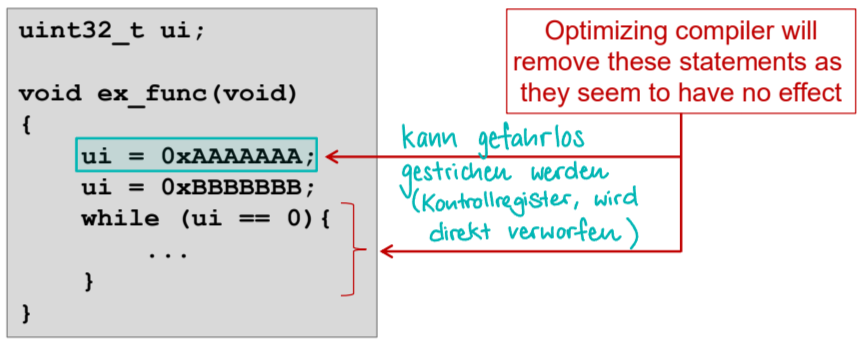
\includegraphics[width=0.7\linewidth]{compiler_problems.png}
    \begin{itemize}
        \item Accesses to control registers (read/write) are memory accesses
        \item If writing has a side effect on the hardware and/or if reading may result in a different value than was set before in the code,
        the program will not behave as intended/expected
    \end{itemize}
\end{concept}

\begin{theorem}{Solution}
    \begin{itemize}
        \item Use the \texttt{volatile} keyword/qualifier in C to prevent the compiler from removing statements that have no effect from the compiler's point of view\\
        $\rightarrow$ prohibit compiler optimizations on the variable\\
        \item The compiler will not optimize away accesses to a variable declared as volatile
        \item The compiler will not reorder accesses to a variable declared as volatile
    \end{itemize}
    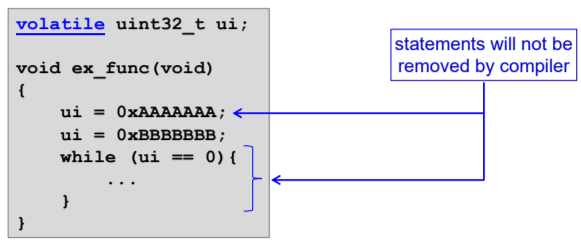
\includegraphics[width=0.7\linewidth]{volatile_keyword.png}
    \begin{itemize}
        \item Tell compiler that the variable may change at any time, outside the control of the compiler (e.g. by hardware or interrupt handler)
        \item The compiler cannot make any assumptions about the value of the variable\\
        needs to execute all read/write accesses as programmed\\
        prevents compiler optimizations
    \end{itemize}
\end{theorem}

\begin{code}{Using volatile for register access}
\begin{lstlisting}[language=C, style=basesmol]
// Without volatile, compiler might remove these statements
uint32_t ui;
void ex_func(void) {
    ui = 0xAAAAAAA;  // Appears to have no effect
    ui = 0xBBBBBBB;  // Appears to have no effect
    while (ui == 0) {
        // ...
    }
}

// With volatile, all accesses are preserved
volatile uint32_t ui;
void ex_func(void) {
    ui = 0xAAAAAAA;  // Will be executed
    ui = 0xBBBBBBB;  // Will be executed
    while (ui == 0) {
        // ...
    }
}
\end{lstlisting}
\end{code}

\begin{KR}{Accessing Registers Through Pointers}
\paragraph{Step 1: Create pointer to register}
Define a pointer to a volatile memory-mapped register.
\paragraph{Step 2: Assign address}
Cast the register's physical address to a pointer type.
\paragraph{Step 3: Access register}
Use pointer dereference to read or write.

\begin{lstlisting}[language=C, style=basesmol]
// Create a pointer to volatile uint32_t
volatile uint32_t *p_reg;

// Set LEDs
p_reg = (volatile uint32_t *)(0x60000100);
*p_reg = 0xAA55AA55;  // Write pattern to LEDs

// Wait for DIP switches to be non-zero
p_reg = (volatile uint32_t *)(0x60000200);
while (*p_reg == 0) {
    // Wait until any switch is pressed
}
\end{lstlisting}
\end{KR}

\begin{corollary}{Access through Pointers} e.g. writing to and reading from CT Board I/O

    \begin{minipage}{0.6\linewidth}
    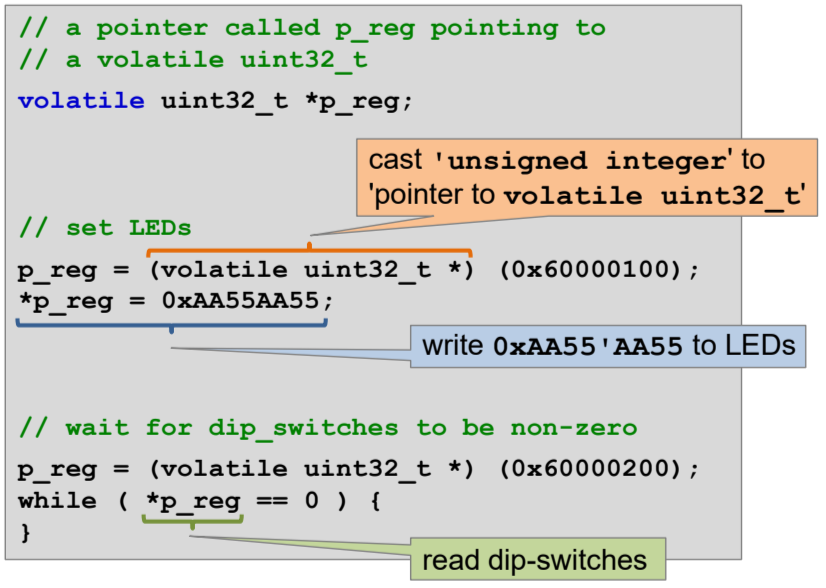
\includegraphics[width=0.9\linewidth]{access_through_pointers1.png}
    \end{minipage}
    \begin{minipage}{0.2\linewidth}
    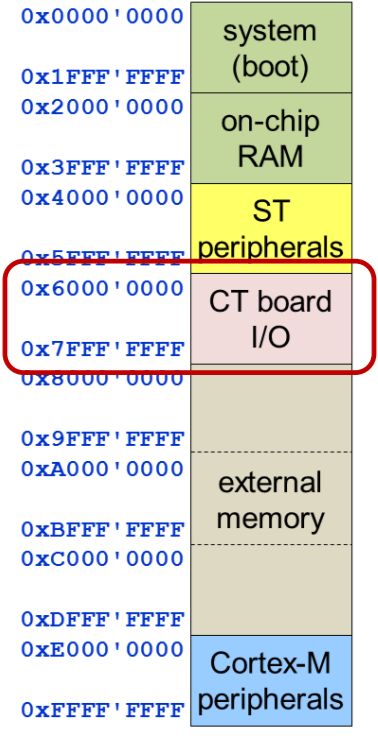
\includegraphics[width=\linewidth]{access_through_pointers2.png}
    \end{minipage}
\end{corollary}

\begin{KR}{Using Preprocessor Macros for Register Access}
\paragraph{Step 1: Define register macros}
Create macros that encapsulate register addresses with proper casting and dereferencing.
\paragraph{Step 2: Use macros for access}
Access registers through the defined macros.

\begin{lstlisting}[language=C, style=basesmol]
// Define register macros
#define LED31_0_REG     (*((volatile uint32_t *)(0x60000100)))
#define BUTTON_REG      (*((volatile uint32_t *)(0x60000210)))

// Write to LED register
LED31_0_REG = 0xBBCCDDEE;

// Read button register
uint32_t aux_var = BUTTON_REG;
\end{lstlisting}
\end{KR}

\begin{examplecode}{Using Preprocessor Macros} $\rightarrow$ \#define
\begin{lstlisting}[language=C, style=basesmol]
#define LED31_0_REG (*((volatile uint32_t *) 0x60000100))

#define BUTTON_REG (*((volatile uint32_t *) 0x60000210))

//Write LED register to 0xBBCC'DDEE
LED31_0_REG = 0xBBCCDDEE;
//Read Button register to aux_var
aux_var = BUTTON_REG;
\end{lstlisting}
    \vspace{2mm}
    \texttt{(\textcolor{darkturquoise}{*}(\textcolor{pink}{(volatile\ uint32\_t *)} 0x60000100))}\\
    $\rightarrow$ \textcolor{darkturquoise}{dereference} the pointer to the register address\\
    $\rightarrow$ \textcolor{pink}{cast} the address to a pointer to a 32-bit register
\end{examplecode}

\raggedcolumns
\columnbreak

\section{Microcontroller Basics Exercises}

\subsection{Bus Access Analysis}

\begin{KR}{Analyzing Bus Cycle Diagrams}
\paragraph{Read access analysis}
\begin{itemize}
    \item Examine clock (CLK), address lines (A), data lines (D), and control signals (NWE, NOE, NE)
    \item Identify whether it's a read (NOE active) or write (NWE active) operation
    \item Note the address value from address lines
    \item For read operations, note the data value returned on data lines
\end{itemize}

\paragraph{Write access analysis}
\begin{itemize}
    \item Identify write operations (NWE active)
    \item Note the address value from address lines
    \item Note the data value being written from data lines
\end{itemize}

\paragraph{Memory mapping}
\begin{itemize}
    \item Remember that processors like ARM use little-endian ordering
    \item Lowest memory address holds the least significant byte (LSB)
    \item Highest memory address in the word holds the most significant byte (MSB)
    \item Map the bytes according to this ordering in memory
\end{itemize}
\end{KR}

\begin{example2}{Bus Cycle Analysis Example}\\
Given the following bus cycle diagram, determine the operation type, address, and data value:

\begin{center}
\begin{tabular}{l}
Access 1: T1 T2 T3 T4 T5 T6 with A[31:0] = 0x6100ABC8, NOE active, D[31:0] = 0x11223344 \\
Access 2: T1 T2 T3 T4 T5 with A[31:0] = 0x6100ABC8, NWE active, D[31:0] = 0x55667788
\end{tabular}
\end{center}

\tcblower
\paragraph{Solution:}
Access 1: This is a read operation because NOE is active.
\begin{itemize}
    \item Address: 0x6100ABC8
    \item Data read: 0x11223344
\end{itemize}

Access 2: This is a write operation because NWE is active.
\begin{itemize}
    \item Address: 0x6100ABC8
    \item Data written: 0x55667788
\end{itemize}

Memory contents (little-endian):
\begin{center}
\begin{tabular}{|c|c|}
\hline
\textbf{Address} & \textbf{Content before Access 2} \\
\hline
0x6100ABC8 & 0x44 (LSB) \\
0x6100ABC9 & 0x33 \\
0x6100ABCA & 0x22 \\
0x6100ABCB & 0x11 (MSB) \\
\hline
\end{tabular}
\quad
\begin{tabular}{|c|c|}
\hline
\textbf{Address} & \textbf{Content after Access 2} \\
\hline
0x6100ABC8 & 0x88 (LSB) \\
0x6100ABC9 & 0x77 \\
0x6100ABCA & 0x66 \\
0x6100ABCB & 0x55 (MSB) \\
\hline
\end{tabular}
\end{center}
\end{example2}

\subsection{Address Decoding}

\begin{KR}{Analyzing Address Decoding Logic}
\paragraph{Identifying addressable range}
\begin{itemize}
    \item Determine the total address space from the number of address lines: $2^n$ bytes
    \item For partial address decoding, identify which address lines are actually decoded
    \item Find which address bits are fixed (compared in the logic) and which are "don't care"
\end{itemize}

\paragraph{Calculating address ranges}
\begin{itemize}
    \item For fully decoded address: Only one specific address activates the select signal
    \item For partially decoded address:
    \begin{itemize}
        \item Identify how many address bits are not decoded ("don't care" bits)
        \item Calculate the number of different addresses that map to the same location: $2^m$ where $m$ is the number of "don't care" bits
        \item Use the fixed bits to determine the base address pattern
        \item Substitute all possible values for the "don't care" bits to find all addresses
    \end{itemize}
\end{itemize}

\paragraph{Creating decoding logic}
\begin{itemize}
    \item For exact address decoding: AND all address bits (or their complements) according to the required pattern
    \item For partial decoding: Only include the relevant address bits in the logic
\end{itemize}
\end{KR}

\begin{example2}{Address Decoding Example}\\
Given a 6-bit address bus A[5:0], determine the addresses that will select a device with the following address decoding logic:
\begin{center}
select = A[5] \& A[4] \& !A[3] \& !A[2]
\end{center}

\tcblower
\paragraph{Solution:}
The decoding logic fixes 4 address bits: A[5:2] = 1100

The bits A[1:0] are "don't care" bits (not included in the logic), giving 4 possible addresses:
\begin{itemize}
    \item A[5:0] = 110000 = 0x30
    \item A[5:0] = 110001 = 0x31
    \item A[5:0] = 110010 = 0x32
    \item A[5:0] = 110011 = 0x33
\end{itemize}

Therefore, the device can be addressed at any of these four addresses: 0x30, 0x31, 0x32, or 0x33.
\end{example2}

\columnbreak

\subsection{Memory-Mapped I/O Access in C}

\begin{KR}{Memory-Mapped Register Access in C}
\paragraph{Define register addresses}
\begin{itemize}
    \item Use \texttt{\#define} for each register address
    \item Create pointer types for each data width (8-bit, 16-bit, 32-bit)
    \item Use \texttt{volatile} qualifier to prevent optimization
\end{itemize}

\paragraph{Reading from registers}
\begin{itemize}
    \item Cast the register address to a volatile pointer of appropriate width
    \item Dereference the pointer to read the value
    \item Use bit masks and shifts to extract specific bits if needed
\end{itemize}

\paragraph{Writing to registers}
\begin{itemize}
    \item Cast the register address to a volatile pointer of appropriate width
    \item Assign a value to the dereferenced pointer to write
    \item For bit manipulation operations:
    \begin{itemize}
        \item Use bitwise OR (|) to set specific bits without affecting others
        \item Use bitwise AND (\&) with inverted mask to clear specific bits
        \item Use bitwise XOR ($\land$) to toggle specific bits
    \end{itemize}
\end{itemize}

\paragraph{Waiting for status bits}
\begin{itemize}
    \item Create a polling loop that checks the status bit
    \item Use appropriate bit masks to isolate the status bit
    \item Use volatile to ensure the register is read on each iteration
\end{itemize}
\end{KR}

\begin{example2}{Memory-Mapped Register Access Example}\\
Write C code to:
\begin{enumerate}
    \item Read an 8-bit control register at address 0x61000007
    \item Set all bits of a 16-bit control register at address 0x61000008 to '1'
    \item Wait until bit 15 in a 32-bit register at address 0x6100000C is set
    \item Set bit 16 in a 32-bit register at address 0x61000010 without changing other bits
\end{enumerate}

\tcblower
\paragraph{Solution:}
\begin{lstlisting}[language=C, style=basesmol]
#include <stdint.h>

// Define register addresses with appropriate types
#define MY_BYTE_REG     (*((volatile uint8_t *)(0x61000007)))
#define MY_HALFWORD_REG (*((volatile uint16_t *)(0x61000008)))
#define MY_WORD_REG     (*((volatile uint32_t *)(0x6100000C)))
#define MY_WORD_REG2    (*((volatile uint32_t *)(0x61000010)))

void register_operations(void) {
    // Read 8-bit control register
    uint8_t my_var = MY_BYTE_REG;
    
    // Set all bits of 16-bit register to '1'
    MY_HALFWORD_REG = 0xFFFF;
    
    // Wait until bit 15 is set in 32-bit register
    while (!(MY_WORD_REG & 0x00008000)) {
        // Empty loop body
    }
    
    // Set bit 16 without changing other bits
    MY_WORD_REG2 |= 0x00010000;
}
\end{lstlisting}
\end{example2}


	\raggedcolumns
	\pagebreak
	\section{GPIO (General Purpose I/O)}

\subsection{GPIO Fundamentals}

\begin{concept}{GPIO Overview}\\
General Purpose Input/Output (GPIO) pins allow the microcontroller to interact with the external world.
\begin{itemize}
    \item Pins can be configured as digital inputs or outputs
    \item Most pins support multiple functions (pin sharing) through internal multiplexers
    \item Configuration is done through memory-mapped registers
    \item Each GPIO port typically has 16 pins (e.g., GPIOA, GPIOB, etc.)
\end{itemize}
\end{concept}

\begin{definition}{Pin Sharing}\\
Multiple functions can share a single physical pin:
\begin{itemize}
    \item Digital inputs/outputs (GPIO)
    \item Serial interfaces (UART, SPI, I2C)
    \item Timers/Counters
    \item ADC (Analog-to-Digital Conversion)
    \item Alternate functions
\end{itemize}
Not all functions can be used simultaneously; configuration registers define pin usage.
\end{definition}

\subsection{GPIO Structure}

\begin{concept}{GPIO Hardware Structure}\\
Each GPIO pin contains several hardware components:
\begin{itemize}
    \item Input data register (IDR) - reads the pin state
    \item Output data register (ODR) - sets the output state
    \item Direction control (MODER) - configures pin as input or output
    \item Output type control (OTYPER) - push-pull or open-drain
    \item Pull-up/pull-down resistors (PUPDR)
    \item Speed configuration (OSPEEDR)
    \item Alternate function selection (AFRL/AFRH)
\end{itemize}
\end{concept}

\begin{definition}{GPIO Registers}\\
Each GPIO port has several configuration registers:
\begin{itemize}
    \item \textbf{GPIOx\_MODER}: Mode register (input, output, alternate function, analog)
    \item \textbf{GPIOx\_OTYPER}: Output type register (push-pull or open-drain)
    \item \textbf{GPIOx\_OSPEEDR}: Output speed register (low, medium, high, very high)
    \item \textbf{GPIOx\_PUPDR}: Pull-up/pull-down register
    \item \textbf{GPIOx\_IDR}: Input data register (read-only)
    \item \textbf{GPIOx\_ODR}: Output data register (read/write)
    \item \textbf{GPIOx\_BSRR}: Bit set/reset register (atomic operations)
    \item \textbf{GPIOx\_LCKR}: Configuration lock register
    \item \textbf{GPIOx\_AFRL/H}: Alternate function registers
\end{itemize}
\end{definition}

\columnbreak

\subsection{GPIO Configuration}

\begin{definition}{Direction Configuration (MODER)}\\
The GPIOx\_MODER register configures each pin's direction:
\begin{itemize}
    \item \textbf{00}: Input mode
    \item \textbf{01}: General purpose output mode
    \item \textbf{10}: Alternate function mode
    \item \textbf{11}: Analog mode
\end{itemize}
Each pin uses 2 bits in the register, allowing for 16 pins per port.
\end{definition}

\begin{definition}{Output Type (OTYPER)}\\
The GPIOx\_OTYPER register configures the output driver type:
\begin{itemize}
    \item \textbf{0}: Push-pull (can actively drive high or low)
    \item \textbf{1}: Open-drain (can drive low, relies on external pull-up for high)
\end{itemize}
\end{definition}

\begin{definition}{Pull-up/Pull-down (PUPDR)}\\
The GPIOx\_PUPDR register configures internal resistors:
\begin{itemize}
    \item \textbf{00}: No pull-up, no pull-down
    \item \textbf{01}: Pull-up
    \item \textbf{10}: Pull-down
    \item \textbf{11}: Reserved
\end{itemize}
\end{definition}

\begin{definition}{Speed Configuration (OSPEEDR)}\\
The GPIOx\_OSPEEDR register configures the output slew rate:
\begin{itemize}
    \item \textbf{00}: Low speed
    \item \textbf{01}: Medium speed
    \item \textbf{10}: High speed
    \item \textbf{11}: Very high speed
\end{itemize}
\end{definition}

\subsection{Push-Pull vs. Open-Drain}

\begin{concept}{Push-Pull vs Open-Drain Outputs}
\begin{itemize}
    \item \textbf{Push-Pull:}
    \begin{itemize}
        \item Can actively drive output high (to VDD) or low (to GND)
        \item Faster switching times, can source and sink current
        \item Default output mode for GPIO pins
    \end{itemize}
    \item \textbf{Open-Drain:}
    \begin{itemize}
        \item Can only actively drive output low
        \item Relies on external pull-up resistor to reach high state
        \item Multiple devices can share a line without conflicts (e.g., I2C bus)
        \item Used in "wired-AND" configurations
    \end{itemize}
\end{itemize}
\end{concept}

\subsection{Data Registers and Operations}

\begin{definition}{Input Data Register (IDR)}\\
The GPIOx\_IDR is a read-only register containing the input value of the corresponding I/O port.
\end{definition}

\begin{definition}{Output Data Register (ODR)}\\
The GPIOx\_ODR can be read and written to set the output state of GPIO pins.
\end{definition}

\begin{definition}{Bit Set/Reset Register (BSRR)}\\
The GPIOx\_BSRR allows atomic bit operations:
\begin{itemize}
    \item Bits [15:0]: Set corresponding ODR bit by writing '1'
    \item Bits [31:16]: Reset corresponding ODR bit by writing '1'
\end{itemize}
This ensures atomic access without read-modify-write operations.
\end{definition}

\begin{KR}{Configuring a GPIO Pin}
\paragraph{Step 1: Enable GPIO clock}
Enable the clock to the GPIO port using RCC register.
\paragraph{Step 2: Configure pin direction}
Set the mode register (MODER) to configure as input, output, etc.
\paragraph{Step 3: Configure additional properties}
Configure output type, speed, and pull-up/down as needed.
\paragraph{Step 4: Set initial state (for outputs)}
For output pins, set the initial state in ODR or using BSRR.

\begin{lstlisting}[language=C, style=basesmol] 
// Step 1: Enable GPIOA clock
RCC->AHB1ENR |= (1 << 0);  // Set bit 0 for GPIOA

// Step 2: Configure PA5 as output (bits 10-11 = 01)
GPIOA->MODER &= ~(3 << 10);  // Clear bits 10-11
GPIOA->MODER |= (1 << 10);   // Set as output

// Step 3: Configure as push-pull, high speed, no pull-up/down
GPIOA->OTYPER &= ~(1 << 5);     // Push-pull (clear bit 5)
GPIOA->OSPEEDR |= (3 << 10);    // Very high speed (set bits 10-11)
GPIOA->PUPDR &= ~(3 << 10);     // No pull-up/down (clear bits 10-11)

// Step 4: Set initial state (turn on LED)
GPIOA->ODR |= (1 << 5);         // Set PA5 high
// OR: Atomic set
GPIOA->BSRR = (1 << 5);         // Set PA5 high
\end{lstlisting}
\end{KR}

\begin{KR}{Reading and Writing GPIO}
\paragraph{Reading Input Pins}
Read the current state of GPIO pins using the IDR register.
\paragraph{Writing Output Pins - Using ODR}
Set or clear output pins by modifying the ODR register.
\paragraph{Writing Output Pins - Using BSRR (preferred)}
Set or clear output pins atomically using the BSRR register.

\begin{lstlisting}[language=C, style=basesmol] 
// Reading input from GPIOA pin 0
uint32_t buttonState = (GPIOA->IDR & (1 << 0)) != 0;

// Writing output using ODR (not atomic)
// Set pin high
GPIOA->ODR |= (1 << 5);
// Set pin low
GPIOA->ODR &= ~(1 << 5);

// Writing output using BSRR (atomic)
// Set pin high (bits 0-15)
GPIOA->BSRR = (1 << 5);
// Set pin low (bits 16-31)
GPIOA->BSRR = (1 << (5 + 16));
\end{lstlisting}
\end{KR}

\begin{example2}{GPIO Configuration Exercise}\\
Configure pin PA3 as an output with open-drain configuration, low speed, and pull-up enabled. Then set the pin to low state.
\begin{lstlisting}[language=C, style=basesmol] 
// Enable GPIOA clock
RCC->AHB1ENR |= (1 << 0);  // Bit 0 for GPIOA

// Configure PA3 as output (bits 6-7 = 01)
GPIOA->MODER \&= ~(3 << 6);  // Clear bits 6-7
GPIOA->MODER |= (1 << 6);   // Set bit 6 (output mode)

// Configure as open-drain (bit 3 = 1)
GPIOA->OTYPER |= (1 << 3);  

// Configure as low speed (bits 6-7 = 00)
GPIOA->OSPEEDR \&= ~(3 << 6);  // Clear bits 6-7 (low speed)

// Configure with pull-up (bits 6-7 = 01)
GPIOA->PUPDR \&= ~(3 << 6);    // Clear bits 6-7
GPIOA->PUPDR |= (1 << 6);     // Set bit 6 (pull-up)

// Set pin to low state using BSRR
GPIOA->BSRR = (1 << (3 + 16));  // Set bit 19 (reset PA3)
\end{lstlisting}
\end{example2}

\subsection{Hardware Abstraction Layer (HAL)}

\begin{concept}{HAL for GPIO}\\
The Hardware Abstraction Layer provides a structured way to access GPIO registers:
\begin{itemize}
    \item Based on structs that map to hardware registers
    \item Typedef for register structure (e.g., \texttt{reg\_gpio\_t})
    \item Pointers to each GPIO port (e.g., \texttt{GPIOA}, \texttt{GPIOB})
    \item Base addresses defined in header file
    \item Helper macros for bit manipulation
\end{itemize}
This approach makes code more readable and maintainable than direct register address manipulation.
\end{concept}

\begin{code}{Using HAL for GPIO}
\begin{lstlisting}[language=C, style=basesmol] 
// Using HAL style access
#include "reg_stm32f4xx.h"  // Contains structure definitions

// Configure PA3 as output
GPIOA->MODER &= ~(3 << 6);  // Clear bits 6-7
GPIOA->MODER |= (1 << 6);   // Set bit 6 (output mode)

// Instead of direct register access:
// volatile uint32_t *reg = (volatile uint32_t *)(0x40020000);
// *reg &= ~(3 << 6);
// *reg |= (1 << 6);
\end{lstlisting}
\end{code}

	\raggedcolumns
	\pagebreak
	\section{Serial Data Transfer}


\mult{2}

\begin{definition}{Serial vs. Parallel Communication}\\
Microcontrollers often use serial connections for communication:

\textbf{Serial Connection}: Data transmitted one bit at a time over fewer wires
    \begin{itemize}
        \item Simpler (saves PCB area)
        \item Reduces number of switching lines (reduced power, improved EMC)
        \item Requires higher-level protocol for interpretation
    \end{itemize}
\textbf{Parallel Bus}: Data transmitted over multiple lines simultaneously
    \begin{itemize}
        \item Faster for short distances
        \item More complex routing
        \item Higher power consumption and EMC issues
    \end{itemize}
\end{definition}

\begin{concept}{Serial Connections} Wires
        \begin{itemize}
            \item Serial \textbf{Data lines:} Carry the actual data
            \item Optional \textbf{Control lines:} Manage communication (e.g., clock, chip select)
        \end{itemize}
        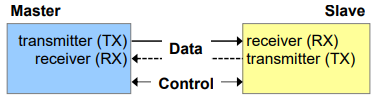
\includegraphics[width=0.8\linewidth]{serialdatatransferconnections.png}
\end{concept}

\begin{concept}{Serial Communication Modes}
\begin{itemize}
    \item \textbf{Simplex}: Unidirectional, one-way only communication
    \item \textbf{Half-duplex}: Bidirectional, but only one direction at a time
    \item \textbf{Full-duplex}: Bidirectional, both directions simultaneously
\end{itemize}
\end{concept}

\begin{concept}{Serial Communication Timing}

    \textbf{Synchronous}: Both nodes use the same clock
    \begin{itemize}
        \item Clock often provided by master
        \item Examples: SPI, I2C
    \end{itemize}
\textbf{Asynchronous}: Each node uses an individual clock
    \begin{itemize}
        \item Start/stop bits used for synchronization
        \item Example: UART
    \end{itemize}
    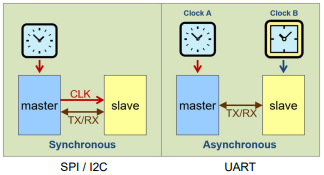
\includegraphics[width=0.8\linewidth]{serialdatatransfertiming.png}
\end{concept}

\multend


\begin{concept}{Overview}\\
    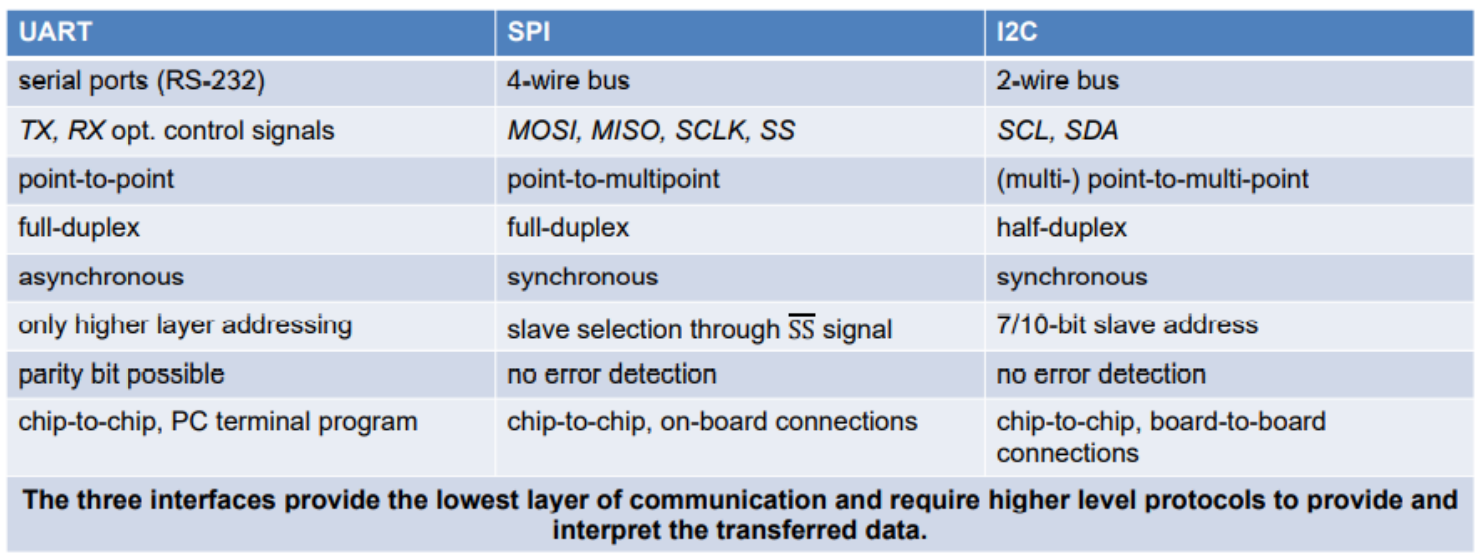
\includegraphics[width=0.9\linewidth]{SDT_overview.png}

    \textbf{SPI - Serial Peripheral Interface}
    \begin{itemize}
        \item Master/slave architecture
        \item Synchronous full-duplex transmissions (MOSI, MISO) with shared clock
        \item Selection of device through Slave Select (SS) $\rightarrow$ multiple slaves possible, !! separate SS line for each slave
        \item no acknowledge, no error detection
        \item Clock signal (SCK) for synchronization: four mode $\rightarrow$ CPOL (clock polarity), CPHA (clock phase)
        \item High speed (up to 50+ Mbps)
    \end{itemize}
    \vspace{2mm}

    \begin{minipage}{0.5\linewidth}
    \textbf{UART - Universal Asynchronous Receiver Transmitter} (Serial Interface)
    \begin{itemize}
        \item Transmitter and receiver use diverging clocks
        \item Asynchronous (no shared clock) $\rightarrow$ synchronization using start and stop bits $\rightarrow$ overhead
        \item longer connections require line drivers \\ $\rightarrow$ RS-232/RS-485
        \item simple wiring (2-3 wires)
        \item Moderate speed (up to ~5 Mbps)
    \end{itemize}
    \end{minipage}
    \hspace{3mm}
    \begin{minipage}{0.45\linewidth}
    \textbf{I2C - Inter-Integrated Circuit}
    \begin{itemize}
        \item Multi-master, multi-slave
        \item Synchronous half-duplex transmission (SCL, SDA) with shared clock - SCL for synchronization
        \item 7-bit slave addresses
        \item Acknowledge, error detection
        \item Medium speed (100 kbps, 400 kbps, up to 5 Mbps)
    \end{itemize}
    \end{minipage}
\end{concept}

\subsection{Protocol Comparison and Selection}

\begin{KR}{Selecting the Appropriate Serial Protocol}
\paragraph{Consider application requirements}
\begin{itemize}
    \item \textbf{Distance:}
    \begin{itemize}
        \item UART with RS-232 levels for longer distances
        \item SPI and I2C typically for on-board connections
    \end{itemize}
    \item \textbf{Speed:}
    \begin{itemize}
        \item SPI for highest speed requirements
        \item I2C for moderate speed with fewer pins
        \item UART for simpler, moderate speed connections
    \end{itemize}
    \item \textbf{Number of devices:}
    \begin{itemize}
        \item I2C for many devices on shared bus
        \item SPI for multiple devices but requires separate SS line for each
        \item UART typically for point-to-point (multiple UARTs needed for multiple devices)
    \end{itemize}
\end{itemize}

\paragraph{Evaluate protocol overhead}
\begin{itemize}
    \item \textbf{UART:} Start, stop, and optional parity bits and requires accurate clock timing
    \item \textbf{SPI:} Minimal protocol overhead, no addressing or acknowledgment
    \item \textbf{I2C:} Start/stop conditions, addressing, and acknowledgment $\rightarrow$ higher overhead, but better error detection
\end{itemize}

\paragraph{Consider hardware support}
\begin{itemize}
    \item Check if target microcontroller has hardware support for chosen protocol
    \item Consider available pins and alternate functions
    \item Evaluate available software libraries and drivers
    \item Consider power requirements (I2C has pull-up resistors that consume power)
\end{itemize}
\end{KR}

\begin{example}
Select the most appropriate serial protocol for each of the following applications:
\begin{enumerate}
    \item A system needs to connect a microcontroller to three temperature sensors. The sensors are low-cost devices that should be replaceable without redesigning the PCB. Data rate requirement is low.
    \item A data acquisition system needs to transfer large amounts of data from an ADC to a microcontroller at 20 Mbps.
    \item A microcontroller needs to communicate with a PC via USB port.
    \item A control system needs to connect to four different devices at varying distances up to 30 meters in an electrically noisy industrial environment.
\end{enumerate}
\paragraph{Solution:}

1. \textbf{I2C is most appropriate for the temperature sensors:}
   \begin{itemize}
     \item Multiple devices (three sensors) can be connected to the same two wires
     \item Each sensor has a unique address, making them individually addressable
     \item Low data rate requirement is well within I2C capabilities
     \item Sensors can be replaced without changing connections (as long as addresses are configured properly)
     \item Reduced pin count (only SCL and SDA) simplifies PCB design
   \end{itemize}
   \vspace{2mm}
2. \textbf{SPI is most appropriate for the high-speed ADC:}
   \begin{itemize}
     \item 20 Mbps data rate exceeds practical I2C speeds and most UART configurations
     \item SPI can easily handle 20+ Mbps with direct hardware support
     \item SPI's full-duplex capability allows simultaneous control and data transfer
     \item Minimal protocol overhead maximizes throughput for large data amounts
     \item Hardware-based chip select ensures proper timing for ADC operations
   \end{itemize}
   \vspace{2mm}
3. \textbf{UART is most appropriate for PC communication:}
   \begin{itemize}
     \item UART is the typical protocol used with USB-to-serial converter chips
     \item Simple point-to-point connection is sufficient for PC communication
     \item Standard baudrates (9600, 115200, etc.) are well-supported by PC software
     \item No need for extra clock signals simplifies interfacing with USB adapters
     \item Asynchronous nature accommodates timing differences between systems
   \end{itemize}
   \vspace{2mm}
4. \textbf{RS-485 (based on UART) is most appropriate for the industrial control system:}
   \begin{itemize}
     \item RS-485 extends UART to longer distances (up to 1200m)
     \item Differential signaling provides excellent noise immunity in industrial environments
     \item Multi-drop capability allows connection to four devices on a single bus
     \item Higher voltage levels offer better signal integrity over 30m distances
     \item Various data rates possible depending on cable length (up to 10 Mbps at shorter distances)
     \item Industry standard protocol with wide hardware support
   \end{itemize}
\end{example}








	\raggedcolumns
	\pagebreak
	
\section{SPI - Serial Peripheral Interface}

\mult{2}

\begin{definition}{SPI}
SPI is a synchronous serial bus primarily for on-board connections:
\begin{itemize}
    \item Used for short-distance communication
    \item Connects microcontroller to external devices (sensors, displays, flash memory, etc.)
\end{itemize}
\end{definition}

\begin{theorem}{SPI Properties}
\begin{itemize}
    \item No defined addressing scheme (uses SS lines instead) $\rightarrow$ KISS (Keep It Simple Stupid)
    \item No built-in acknowledgment or error detection (implemented in higher-level protocols)
    \item Originally for single-byte transfers 
    \begin{itemize}
            \item $\overline{SS}$ deactivated after each byte
            \item Today also used for streams 
    \end{itemize}
    \item Flexible data rate (clock signal is transmitted with data)
    \item No flow control (master controls timing, slave cannot influence)
    \item Susceptible to noise (spikes on clock signal)
\end{itemize}
\end{theorem}

\begin{corollary}{SPI Signals}
\begin{itemize}
    \item \textbf{SCLK} (Serial Clock): Generated by master
    \item \textbf{MOSI} (Master Out Slave In)
    \item \textbf{MISO} (Master In Slave Out)
    \item \textbf{SS/CS} (Slave Select/Chip Select)
\end{itemize}
\end{corollary}

\begin{concept}{SPI Master-Slave Architecture}
\begin{itemize}
    \item Master generates common clock signal (SCLK) for all slaves
    \item Slaves: Selectable by Slave Select (SS) signal 
        \begin{itemize}
            \item Individual Select $\overline{SS1}$, $\overline{SS2}$, $\overline{SS3}$
            \item $\overline{SSx}$ = 1 $\rightarrow$ slave output MISOx is tri-state 
        \end{itemize}
    \item MOSI line connects to inputs of all slaves
    \item MISO lines from all slaves are connected to a single master input
    \item Inactive slaves (SS = '1') put their MISO line in tri-state (high impedance)
    \item Only one selected slave drives its MISO line at a time
\end{itemize}
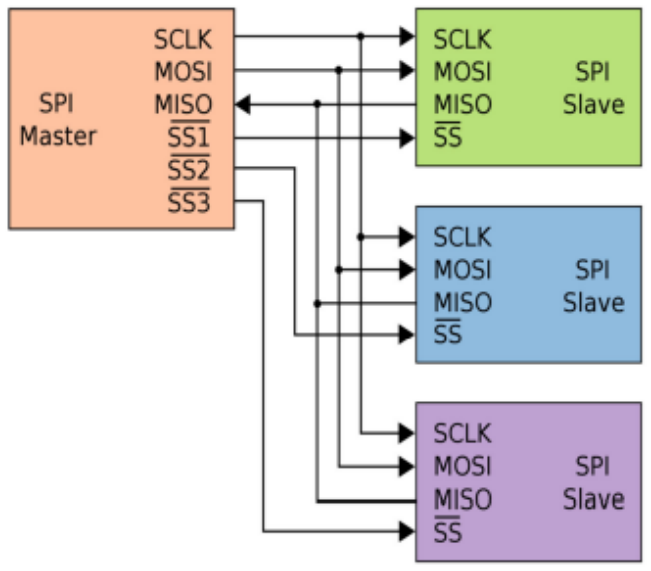
\includegraphics[width=0.6\linewidth]{single_master_mult_slaves.png}
\end{concept}





\multend




\subsubsection{SPI Modes and Timing}

\begin{concept}{Clock Polarity and Phase}
SPI has four different modes based on two parameters:

\begin{minipage}{0.5\linewidth}
\textbf{CPOL} (Clock Polarity): Idle state of clock
    \begin{itemize}
        \item CPOL = 0: Clock idles at low level
        \item CPOL = 1: Clock idles at high level
    \end{itemize}
\end{minipage}
\begin{minipage}{0.5\linewidth}
\textbf{CPHA} (Clock Phase): Which edge is used for data sampling
    \begin{itemize}
        \item CPHA = 0: Data sampled on first clock edge
        \item CPHA = 1: Data sampled on second clock edge
    \end{itemize}
\end{minipage}
\end{concept}

\begin{concept}{Four SPI Modes}

\begin{minipage}{0.5\linewidth}
\textbf{Mode 0}: CPOL = 0, CPHA = 0
    \begin{itemize}
        \item Clock idles low
        \item Data sampled on rising edge, changed on falling edge
    \end{itemize}
\textbf{Mode 1}: CPOL = 0, CPHA = 1
    \begin{itemize}
        \item Clock idles low
        \item Data sampled on falling edge, changed on rising edge
    \end{itemize}
\end{minipage}
\begin{minipage}{0.5\linewidth}
\textbf{Mode 2}: CPOL = 1, CPHA = 0
    \begin{itemize}
        \item Clock idles high
        \item Data sampled on falling edge, changed on rising edge
    \end{itemize}
\textbf{Mode 3}: CPOL = 1, CPHA = 1
    \begin{itemize}
        \item Clock idles high
        \item Data sampled on rising edge, changed on falling edge
    \end{itemize}
\end{minipage}
\end{concept}

\begin{center}
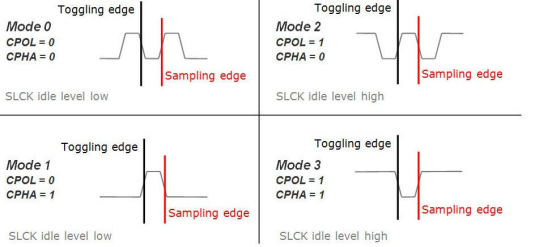
\includegraphics[width=0.75\linewidth]{spi_timing_kr.png}
\end{center}


\begin{KR}{SPI Timing-Diagramm zeichnen}

    \begin{minipage}{0.6\linewidth}
    \paragraph{SPI-Modi (CPOL/CPHA)}
    \begin{itemize}
        \item Mode 0: CPOL=0, CPHA=0 (Idle=Low, Sample=Rising)
        \item Mode 1: CPOL=0, CPHA=1 (Idle=Low, Sample=Falling)
        \item Mode 2: CPOL=1, CPHA=0 (Idle=High, Sample=Falling)
        \item Mode 3: CPOL=1, CPHA=1 (Idle=High, Sample=Rising)
    \end{itemize}
    \end{minipage}
    \hspace{2mm}
    \begin{minipage}{0.35\linewidth}    
    \paragraph{Signale}
    \begin{itemize}
        \item SS (Slave Select): \\ aktiv-low, Slave-Auswahl
        \item SCLK: Clock vom Master
        \item MOSI: Master Out Slave In
        \item MISO: Master In Slave Out
    \end{itemize}
    \end{minipage}
    
    \paragraph{Timing zeichnen}

    \begin{minipage}{0.6\linewidth}
    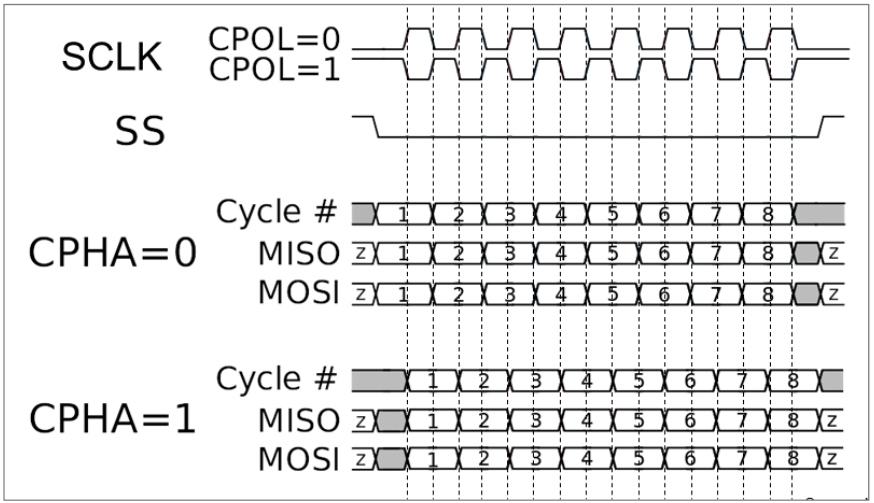
\includegraphics[width=\linewidth]{SPI_communication.png}
    \end{minipage}
    \begin{minipage}{0.35\linewidth}
    \begin{enumerate}
        \item SCLK entsprechend CPOL \\ (Idle-Level)
        \item SS aktiv (low) \\ für gesamte Übertragung
        \item Daten auf MOSI/MISO je nach CPHA (Toggling Edge)
        \item MOSI: Data from Master to Slave
        \item MISO: Data from Slave to Master
        \item Sampling Edges markieren basierend auf CPHA
    \end{enumerate}
    \end{minipage}

    \paragraph{Calculate timing parameters}
    \begin{itemize}
        \item Bit cell time = 1/clock\_frequency
        \item Frame time = (number\_of\_bits)/clock\_frequency
        \item Example: 8 bits at 100 kHz = 80 µs per frame
    \end{itemize}

\end{KR}

\begin{example2}{SPI Mode 3 Timing}\\
    \begin{minipage}{0.5\linewidth}
    SPI Interface mit 8 Bit Daten:
    \begin{itemize}
        \item MOSI: 0xA7 (10100111b)
        \item MISO: 0x37 (00110111b)
    \end{itemize}
    \end{minipage}
    \begin{minipage}{0.5\linewidth}
    \begin{itemize}
        \item Mode 3: CPOL=1, CPHA=1
        \item MSB first
        \item SCLK: 100kHz
    \end{itemize}
    \end{minipage}
    
    \textbf{Timing-Diagramm:}
    \begin{center}
    \includegraphics[width=0.8\linewidth]{spi_timing_ex.png}
    \end{center}

    \begin{minipage}{0.5\linewidth}
        \textbf{Timing-Charakteristika:}
    \begin{itemize}
        \item SCLK Idle = High (CPOL=1)
        \item Daten wechseln auf steigende Flanke (CPHA=1)
        \item Sampling auf fallende Flanke
        \item Bit-Zeit = 1/100kHz = 0.01 ms = 10 $\mu$s
    \end{itemize}
    \end{minipage}
    \begin{minipage}{0.5\linewidth}
        \textbf{Daten-Übertragung:}
    \begin{itemize}
        \item SS: Low waehrend gesamter Uebertragung
        \item SCLK: startet High, 8 Taktzyklen
        \item MOSI: 1-0-1-0-0-1-1-1 (MSB first)
        \item MISO: 0-0-1-1-0-1-1-1 (MSB first)
    \end{itemize}
    \end{minipage}
\end{example2}

\begin{remark}
    Bei SPI ist die Uebertragung immer full-duplex - Master und Slave senden gleichzeitig. Auch wenn nur in eine Richtung Daten benoetigt werden, findet auf der anderen Leitung eine "Dummy"-Uebertragung statt.
\end{remark}









\subsection{SPI Implementation}

\begin{concept}{SPI Implementation Using Shift Registers}
\begin{itemize}
    \item Both master and slave contain 8-bit shift registers
    \item Bits are shifted out on one clock edge (toggling edge)
    \item Bits are sampled on the other clock edge (sampling edge)
    \item 8 clock cycles exchange 8 bits in each direction simultaneously
    \item After 8 clock cycles, data has been exchanged in both directions
    \item Status flags (TXE, RXNE) indicate buffer status
\end{itemize}
\end{concept}

\subsubsection{STM32 SPI Implementation}

\begin{concept}{STM32 SPI Architecture}
The STM32F4 SPI peripheral includes:
\begin{itemize}
    \item Configuration registers (SPI\_CR1, SPI\_CR2)
    \item Status register (SPI\_SR)
    \item Data register (SPI\_DR) for transmit and receive
    \item Status flags for synchronization (TXE, RXNE, BSY)
    \item Support for different communication modes
    \item DMA capability for high-speed transfers
\end{itemize}
\end{concept}

\begin{code}{STM32 SPI Register Configuration}
\begin{lstlisting}[language=C, style=basesmol]
// SPI configuration example
// Configure SPI1 in master mode, CPOL=1, CPHA=1, 8-bit data

// Enable SPI1 clock
RCC->APB2ENR |= RCC_APB2ENR_SPI1EN;

// Configure SPI1
SPI1->CR1 = (1 << 0)   // CPHA=1
          | (1 << 1)   // CPOL=1
          | (1 << 2)   // Master mode
          | (3 << 3)   // BR[2:0]=011: fPCLK/16 (prescaler)
          | (0 << 7)   // MSB first (LSBFIRST=0)
          | (1 << 8)   // SSI=1 (needed for software SS)
          | (1 << 9);  // SSM=1 (software slave management)

// Enable SPI
SPI1->CR1 |= (1 << 6); // SPE=1 (SPI enable)
\end{lstlisting}
\end{code}

\begin{KR}{Transmitting Data with SPI}
\paragraph{Step 1: Prepare SPI}
Configure and enable the SPI peripheral.
\paragraph{Step 2: Check TXE flag}
Wait until the transmit buffer is empty.
\paragraph{Step 3: Write data}
Write data to the data register.
\paragraph{Step 4: Wait for completion}
Wait until transmission is complete by checking BSY flag.

\begin{lstlisting}[language=C, style=basesmol]
// Transmit a byte over SPI
uint8_t transmit_byte(uint8_t data) {
    // Step 1: SPI should already be configured
    
    // Step 2: Wait until TXE=1 (transmit buffer empty)
    while (!(SPI1->SR & (1 << 1))) { }
    
    // Step 3: Write data to transmit
    SPI1->DR = data;
    
    // Step 4: Wait for reception (needed to get received data)
    while (!(SPI1->SR & (1 << 0))) { }
    
    // Return received data (read DR clears RXNE flag)
    return SPI1->DR;
}
\end{lstlisting}
\end{KR}

\begin{KR}{Handling Full-Duplex SPI Communication}
\paragraph{Step 1: Enable SPI with SPE bit}
Ensure SPI is properly configured and enabled.
\paragraph{Step 2: Write first byte to transmit}
Write the first byte to DR to start transmission/reception.
\paragraph{Step 3: Process data in a loop}
Check TXE and RXNE flags to handle both transmission and reception.
\paragraph{Step 4: Wait for completion}
Wait for BSY=0 to ensure all transfers are complete.

\begin{lstlisting}[language=C, style=basesmol]
// Full-duplex SPI communication
void spi_transfer(uint8_t *tx_data, uint8_t *rx_data, uint16_t length) {
    // Enable SPI
    SPI1->CR1 |= (1 << 6);  // SPE=1
    
    // Write first TX byte to start transmission
    if (length > 0) {
        SPI1->DR = tx_data[0];
    }
    
    uint16_t tx_count = 1;
    uint16_t rx_count = 0;
    
    // Process data
    while (rx_count < length) {
        // Check if we can transmit more data
        if ((tx_count < length) && (SPI1->SR & (1 << 1))) {  // TXE=1
            SPI1->DR = tx_data[tx_count++];
        }
        
        // Check if we received data
        if (SPI1->SR & (1 << 0)) {  // RXNE=1
            rx_data[rx_count++] = SPI1->DR;
        }
    }
    
    // Wait until BSY=0 (SPI not busy)
    while (SPI1->SR & (1 << 7)) { }
}
\end{lstlisting}
\end{KR}

\begin{concept}{Synchronizing Hardware and Software}
    \begin{itemize}
        \item TXE (TX Buffer Empty) $\rightarrow$ Software can write next TX Byte to SPI\_DR
        \item RXNE (RX Buffer Not Empty) $\rightarrow$ a byte has been received. Software can read it from SPI\_DR
        \item BSY (Busy) $\rightarrow$ Transmission in progress
    \end{itemize}
    \includegraphics[width=\linewidth]{transmitting_spi.png}\\
    \includegraphics[width=\linewidth]{receiving_spi.png}
\end{concept}
    
	\raggedcolumns
	\pagebreak
	\section{Serial Data Transfer - UART \& I2C}

\subsection{UART Fundamentals}

\mult{2}

\begin{concept}{UART - Universal Asynchronous Receiver Transmitter}\\
UART is an asynchronous serial communication interface:
\begin{itemize}
    \item Asynchronous - no shared clock between transmitter and receiver
    \item Point-to-point communication (one transmitter, one receiver)
    \item Full-duplex (simultaneous bidirectional communication)
    \item Start and stop bits used for synchronization
    \item Typically 2-wire interface (TX and RX) for data
    \item Optional control signals (RTS/CTS, etc.) for flow control
\end{itemize}
\end{concept}

\begin{definition}{UART Signals}\\
Basic UART connections require:
\begin{itemize}
    \item \textbf{TX} (Transmit): Data output from transmitter to receiver
    \item \textbf{RX} (Receive): Data input from transmitter to receiver
    \item \textbf{GND} (Ground): Common reference level
\end{itemize}
Extended UART (with hardware flow control) may include:
\begin{itemize}
    \item \textbf{RTS} (Request to Send): Output indicating readiness to send
    \item \textbf{CTS} (Clear to Send): Input indicating partner is ready to receive
\end{itemize}
\end{definition}

\multend

\subsection{UART Data Format and Timing}

\mult{2}

\begin{definition}{UART Frame Structure}\\
A UART frame consists of:
\begin{itemize}
    \item \textbf{Idle state}: Line is high ('1') when no transmission occurs
    \item \textbf{Start bit}: Always '0', indicates beginning of frame
    \item \textbf{Data bits}: 5 to 9 bits (typically 8), LSB first
    \item \textbf{Parity bit} (optional): For error detection
    \item \textbf{Stop bit(s)}: 1, 1.5, or 2 bits, always '1'
\end{itemize}
\end{definition}

\begin{concept}{UART Synchronization}\\
Without a common clock, UART devices synchronize as follows:
\begin{itemize}
    \item Receiver detects start bit (falling edge from idle to '0')
    \item Receiver samples middle of each bit based on configured baud rate
    \item Both devices must use the same configuration:
    \begin{itemize}
        \item Baud rate (e.g., 9600, 115200 bits/s)
        \item Number of data bits (5-8)
        \item Parity (none, odd, even, mark, space)
        \item Number of stop bits (1, 1.5, 2)
    \end{itemize}
\end{itemize}
\end{concept}

\begin{example2}{UART Timing Diagram Analysis}\\
Given a UART signal with 8 data bits, no parity, 1 stop bit, analyze this pattern:
\\
$\overline{\text{\_\_\_\_\_}}$ $\overline{\text{\_\_}}$ $\overline{\text{\_\_\_\_}}$ $\overline{\text{\_\_}}$ $\overline{\text{\_\_\_\_}}$ $\overline{\text{\_\_\_\_\_\_\_\_\_\_}}$
\\
I I S D D D D D D D D E I I
\\
Where I=Idle, S=Start, D=Data, E=Stop
\tcblower
Breaking down this signal:
- Idle (high) $\rightarrow$ Start bit (low) $\rightarrow$ 8 data bits $\rightarrow$ Stop bit (high) $\rightarrow$ Idle (high)
- Reading data bits (LSB first): 01010011
- Converting to binary: 0b01010011 = 0x53 = ASCII 'S'

This UART transmission contains the character 'S'.
\end{example2}

\begin{formula}{UART Calculations}\\
\textbf{Bit Time (seconds):}
$T_{bit} = \frac{1}{\text{Baud Rate}}$


\textbf{Frame Time (seconds):}
$T_{frame} =$\\$T_{bit} \times (1 + \text{Data Bits} + \text{Parity Bits} + \text{Stop Bits})$


\textbf{Maximum Data Rate (bytes/second):}\\
$\text{Data Rate} = \frac{\text{Baud Rate}}{\text{Total Bits per Byte}}$

where Total Bits per Byte = 1 (start) + Data Bits + Parity Bits + Stop Bits
\end{formula}

\begin{KR}{Clock Tolerance in UART}
\paragraph{Maximum clock deviation}
The receiver must sample correctly until the last bit:
\paragraph{Formula}
Maximum allowed clock deviation (as percentage):
$\text{Deviation}_{\max} = \frac{0.5}{N} \times 100\%$

where N is the number of bit times between synchronization points.
\end{KR}

\begin{example}
    For a standard UART frame (1 start, 8 data, 1 stop):\\
    Synchronization occurs at start bit,
    Last bit (stop bit) is 10 bits later\\
    Maximum clock deviation = 0.5/10 = 5\%\\
    Sample calculation:\\
    If sender clock is 9600 Hz: Receiver can be between 9120 Hz and 10080 Hz
\end{example}

\multend


\subsection{UART on STM32F4}

\begin{concept}{STM32F4 UART/USART Peripherals}\\
The STM32F4 includes several UART/USART modules with features:
\begin{itemize}
    \item Full-duplex communication (USART)
    \item Programmable baud rate
    \item Configurable data bits, stop bits, and parity
    \item Interrupt generation on events (TX empty, RX not empty, etc.)
    \item DMA support for efficient data transfer
    \item Hardware flow control (CTS/RTS) on USARTs
    \item Synchronous mode available on USARTs
\end{itemize}
\end{concept}

\begin{code}{STM32F4 UART Configuration} Configure UART2 for 115200 baud, 8-N-1
\begin{lstlisting}[language=C, style=basesmol]
// 1. Enable UART2 and GPIO clock
RCC->APB1ENR |= RCC_APB1ENR_USART2EN;  // Enable UART2 clock
RCC->AHB1ENR |= RCC_AHB1ENR_GPIOAEN;   // Enable GPIOA clock
// 2. Configure GPIO pins for UART (PA2 = TX, PA3 = RX)
// Set alternate function mode (0x10)
GPIOA->MODER &= ~(0x3 << (2*2) | 0x3 << (2*3));
GPIOA->MODER |= (0x2 << (2*2) | 0x2 << (2*3));
// Set to AF7 (UART2)
GPIOA->AFR[0] &= ~(0xF << (4*2) | 0xF << (4*3));
GPIOA->AFR[0] |= (0x7 << (4*2) | 0x7 << (4*3));
// 3. Configure UART
// Reset UART configuration
USART2->CR1 = 0;
USART2->CR2 = 0;
USART2->CR3 = 0;
// Set baud rate (assuming 84MHz APB1 clock)
// BRR = f_CK / baud rate = 84,000,000 / 115,200 = 729.16
USART2->BRR = 729;
// Enable UART, TX, and RX
USART2->CR1 = USART_CR1_UE | USART_CR1_TE | USART_CR1_RE;
\end{lstlisting}
\end{code}

\begin{KR}{UART Data Transmission and Reception}
\textbf{Transmitting Data}
Write data to the data register after checking the TXE flag.\\
\textbf{Receiving Data}
Read from the data register after checking the RXNE flag.

\begin{lstlisting}[language=C, style=basesmol]
// Send a character
void UART_SendChar(USART_TypeDef *uart, char c) {
    // Wait until TXE flag is set (transmit buffer empty)
    while (!(uart->SR & USART_SR_TXE)) { }
    // Write the character to the data register
    uart->DR = c;
}
// Send a string
void UART_SendString(USART_TypeDef *uart, const char *str) {
    while (*str) {
        UART_SendChar(uart, *str++);
    }
}
// Receive a character (blocking)
char UART_ReceiveChar(USART_TypeDef *uart) {
    // Wait until RXNE flag is set (data received)
    while (!(uart->SR & USART_SR_RXNE)) { }
    // Return received data
    return uart->DR;
}
\end{lstlisting}
\end{KR}


\subsection{I2C Fundamentals}

\begin{concept}{I2C - Inter-Integrated Circuit}\\
I2C is a synchronous, half-duplex, multi-master bus:
\begin{itemize}
    \item Developed by Philips (now NXP) in 1982
    \item 2-wire interface (SCL and SDA)
    \item Multi-master, multi-slave capability
    \item Unique 7-bit or 10-bit address for each device
    \item Synchronous (master provides clock)
    \item Half-duplex (data flows in one direction at a time)
    \item Well-suited for connecting multiple boards or chips
    \item Bit rates from 100 kbit/s (standard) to 5 Mbit/s (ultra-fast)
\end{itemize}
\end{concept}

\begin{definition}{I2C Signals}\\
I2C requires just two bidirectional lines with pull-up resistors:
\begin{itemize}
    \item \textbf{SCL} (Serial Clock Line): Clock signal generated by master
    \item \textbf{SDA} (Serial Data Line): Bidirectional data line
\end{itemize}
Both lines are open-drain, requiring external pull-up resistors.
\end{definition}

\subsection{I2C Protocol}

\begin{concept}{I2C Bus Conditions}\\
Special conditions on the I2C bus:
\begin{itemize}
    \item \textbf{START condition}: SDA goes from high to low while SCL is high
    \item \textbf{STOP condition}: SDA goes from low to high while SCL is high
    \item \textbf{Data valid}: SDA remains stable while SCL is high
    \item \textbf{Data change}: SDA changes only when SCL is low
\end{itemize}
\end{concept}

\begin{definition}{I2C Data Transfer}\\
Data transfer sequence:
\begin{itemize}
    \item Master initiates transfer with START condition
    \item Master sends 7-bit slave address + R/W bit (0 = write, 1 = read)
    \item Addressed slave acknowledges (ACK) by pulling SDA low
    \item Data bytes transferred (8 bits followed by ACK/NACK)
    \item Master terminates transfer with STOP condition
\end{itemize}
Data is transferred MSB first, with the receiver acknowledging each byte.
\end{definition}

\begin{concept}{I2C Acknowledge and Not-Acknowledge}\\
After each byte transfer:
\begin{itemize}
    \item \textbf{ACK} (Acknowledge): Receiver pulls SDA low during 9th clock cycle
    \item \textbf{NACK} (Not-Acknowledge): SDA remains high during 9th clock cycle
\end{itemize}
NACK can indicate:
\begin{itemize}
    \item No receiver with the transmitted address
    \item Receiver unable to receive or transmit
    \item Receiver doesn't understand the data/command
    \item Receiver cannot receive more data
    \item Master-receiver signals end of transfer to slave-transmitter
\end{itemize}
\end{concept}

\begin{example2}{I2C Write Operation}\\
Master wants to write data 0x9C to slave with address 0x66
\tcblower
1. Master generates START condition
2. Master sends slave address (0x66) with R/W = 0 (write): 0xCC
3. Slave acknowledges (ACK)
4. Master sends data byte 0x9C
5. Slave acknowledges (ACK)
6. Master generates STOP condition

I2C bus:
START - 0xCC - ACK - 0x9C - ACK - STOP
\end{example2}

\begin{example2}{I2C Read Operation}\\
Master wants to read data from slave with address 0x66
\tcblower
1. Master generates START condition
2. Master sends slave address (0x66) with R/W = 1 (read): 0xCD
3. Slave acknowledges (ACK)
4. Slave sends data byte (e.g., 0x9C)
5. Master sends NACK to indicate end of transfer
6. Master generates STOP condition

I2C bus:
START - 0xCD - ACK - 0x9C - NACK - STOP
\end{example2}

\subsection{I2C on STM32F4}

\begin{concept}{STM32F4 I2C Peripherals}\\
The STM32F4 includes I2C modules with features:
\begin{itemize}
    \item Compatible with I2C standard protocol
    \item Multiple speed modes (standard, fast)
    \item 7-bit and 10-bit addressing
    \item Multi-master capability
    \item Programmable clock stretching
    \item Programmable NOSTRETCH capability
    \item DMA support for efficient data transfer
    \item SMBus support
\end{itemize}
\end{concept}

\begin{code}{STM32F4 I2C Configuration}
\begin{lstlisting}[language=C, style=basesmol]
// Configure I2C1 for 100kHz standard mode

// 1. Enable I2C1 and GPIO clock
RCC->APB1ENR |= RCC_APB1ENR_I2C1EN;   // Enable I2C1 clock
RCC->AHB1ENR |= RCC_AHB1ENR_GPIOBEN;  // Enable GPIOB clock

// 2. Configure GPIO pins for I2C (PB6 = SCL, PB7 = SDA)
// Set alternate function mode (0x10)
GPIOB->MODER &= ~(0x3 << (2*6) | 0x3 << (2*7));
GPIOB->MODER |= (0x2 << (2*6) | 0x2 << (2*7));

// Set open-drain output type
GPIOB->OTYPER |= (1 << 6) | (1 << 7);

// Set to AF4 (I2C1)
GPIOB->AFR[0] &= ~(0xF << (4*6) | 0xF << (4*7));
GPIOB->AFR[0] |= (0x4 << (4*6) | 0x4 << (4*7));

// 3. Reset I2C
I2C1->CR1 = I2C_CR1_SWRST;  // Software reset
I2C1->CR1 = 0;              // Clear reset

// 4. Configure I2C
// Set peripheral clock frequency (42MHz)
I2C1->CR2 = 42;  // FREQ = 42MHz

// Set CCR for 100kHz standard mode
// CCR = PCLK1 / (2 * I2C_FREQ) = 42MHz / (2 * 100kHz) = 210
I2C1->CCR = 210;

// Set TRISE
// TRISE = (max rise time * PCLK1) + 1 = (1000ns * 42MHz) + 1 = 43
I2C1->TRISE = 43;

// 5. Enable I2C
I2C1->CR1 |= I2C_CR1_PE;  // Peripheral enable
\end{lstlisting}
\end{code}

\begin{KR}{I2C Master Transmit and Receive}
\paragraph{Master Transmit Sequence}
Generate START, send address+write, send data bytes, generate STOP.
\paragraph{Master Receive Sequence}
Generate START, send address+read, receive data bytes with ACK/NACK, generate STOP.

\begin{lstlisting}[language=C, style=basesmol]
// I2C Master Transmit
void I2C_MasterTransmit(I2C_TypeDef *i2c, uint8_t address, uint8_t *data, uint16_t size) {
    // 1. Wait until I2C bus is free
    while (i2c->SR2 & I2C_SR2_BUSY) { }
    
    // 2. Generate START condition
    i2c->CR1 |= I2C_CR1_START;
    
    // 3. Wait for EV5 (START sent)
    while (!(i2c->SR1 & I2C_SR1_SB)) { }
    
    // 4. Send slave address (write mode)
    i2c->DR = address << 1;  // Address + Write bit (0)
    
    // 5. Wait for EV6 (address sent)
    while (!(i2c->SR1 & I2C_SR1_ADDR)) { }
    
    // 6. Clear ADDR by reading SR2
    (void)i2c->SR2;
    
    // 7. Send data bytes
    for (uint16_t i = 0; i < size; i++) {
        // Wait until TXE is set
        while (!(i2c->SR1 & I2C_SR1_TXE)) { }
        
        // Send data byte
        i2c->DR = data[i];
    }
    
    // 8. Wait for transfer to complete
    while (!(i2c->SR1 & I2C_SR1_TXE) || !(i2c->SR1 & I2C_SR1_BTF)) { }
    
    // 9. Generate STOP condition
    i2c->CR1 |= I2C_CR1_STOP;
}
\end{lstlisting}
\end{KR}

\subsection{Comparison of Serial Interfaces}

\begin{concept}{UART vs. SPI vs. I2C Comparison}
\begin{center}
\begin{tabular}{|p{2.5cm}|p{4cm}|p{4cm}|p{4cm}|}
\hline
\textbf{Feature} & \textbf{UART} & \textbf{SPI} & \textbf{I2C} \\
\hline
Wires & 2 (TX, RX) & 4 (MOSI, MISO, SCLK, SS) & 2 (SDA, SCL) \\
\hline
Clock & Asynchronous & Synchronous & Synchronous \\
\hline
Connection Type & Point-to-point & Point-to-multipoint & Multi-point \\
\hline
Duplex & Full-duplex & Full-duplex & Half-duplex \\
\hline
Addressing & Higher layer only & Device selection via SS & 7/10-bit addressing \\
\hline
Error Detection & Optional parity bit & None & ACK/NACK \\
\hline
Speed & Up to ~5 Mbps & Up to ~50 Mbps & 100 kbps to 5 Mbps \\
\hline
Master/Slave & Peer-to-peer & Single master, multiple slaves & Multiple masters, multiple slaves \\
\hline
Typical Use & Terminal communication, debug ports & On-board high-speed communication & Board-to-board, chip-to-chip \\
\hline
\end{tabular}
\end{center}
\end{concept}

\section{Serial Data Transfer}

\begin{concept}{Overview}\\
    \includegraphics[width=\linewidth]{SDT_overview.png}
    \vspace{2mm}\\
    \textbf{SPI - Serial Peripheral Interface}
    \begin{itemize}
        \item Master/slave
        \item Synchronous full-duplex transmissions (MOSI, MISO)
        \item Selection of device through Slave Select (SS)
        \item no acknowledge, no error detection
        \item Clock signal (SCK) for synchronization: four mode $\rightarrow$ CPOL (clock polarity), CPHA (clock phase)
    \end{itemize}
    \vspace{2mm}

    \textbf{UART - Universal Asynchronous Receiver Transmitter} (Serial Interface)
    \begin{itemize}
        \item Transmitter and receiver use diverging clocks
        \item synchronization using start and stop bits $\rightarrow$ overhead
        \item longer connections require line drivers $\rightarrow$ RS-232/RS-485
    \end{itemize}
    \vspace{2mm}

    \textbf{I2C - Inter-Integrated Circuit}
    \begin{itemize}
        \item Synchronous half-duplex transmission (SCL, SDA)
        \item 7-bit slave addresses
        \item Acknowledge, error detection
        \item Clock signal (SCL) for synchronization
    \end{itemize}
\end{concept}

\begin{definition}{Single Master - Multiple Slaves}
    \begin{itemize}
        \item Master generates a common clock signal for all Slaves
        \item MOSI: From Master Output to all Slave Inputs
        \item MISO: From Master Input to all Slave Outputs $\rightarrow$ all slave outpuzs connected to single master input
        \item Slaves: Selectable by Slave Select (SS) signal
        \begin{itemize}
            \item Individual Select $\overline{SS1}$, $\overline{SS2}$, $\overline{SS3}$
            \item $\overline{SSx}$ = 1 $\rightarrow$ slave output MISOx is tri-state 
        \end{itemize}
    \end{itemize}
    \includegraphics[width=\linewidth]{single_master_mult_slaves.png}
\end{definition}

\begin{formula}{Clock Polarity (CPOL) Clock Phase (CPHA)}
    \begin{itemize}
        \item \textbf{CPOL:} Clock Polarity
        \begin{itemize}
            \item 0: Clock is low in idle state
            \item 1: Clock is high in idle state
        \end{itemize}
        \item \textbf{CPHA:} Clock Phase
        \begin{itemize}
            \item 0: Data is sampled on the first edge of the clock
            \item 1: Data is sampled on the second edge of the clock
        \end{itemize}
    \end{itemize}
    \includegraphics[width=\linewidth]{clockpolarity.png}
    \begin{itemize}
        \item TX provides data on \oq Toggling Edge\cq
        \item RX takes over data with \oq Sampling Edge\cq
    \end{itemize}
\end{formula}

\subsection{Serial Connection - SPI}

\begin{definition}{Properties of SPI}
    \begin{itemize}
        \item No defined addressing scheme
        \begin{itemize}
            \item Use of $\overline{SS}$ instead $\rightarrow$ KISS (Keep It Simple Stupid)
        \end{itemize}
        \item Transmission without receive acknowledge and error detection
        \begin{itemize}
            \item Has to be implemented in higher level protocols
        \end{itemize}
        \item Originally used only for transmission of single bytes
        \begin{itemize}
            \item $\overline{SS}$ deactivated after each byte
            \item Today also used for streams 
        \end{itemize}
        \item Data rate: Highly flexible as clock signal is transmitted
        \item No flow-control available
        \begin{itemize}
            \item Master can delay the next clock edge
            \item Slave can't influence the data rate
        \end{itemize}
        \item Susceptible to noise (spikes on clock signal)
    \end{itemize}
\end{definition}

\begin{example2}{SPI - Serial Peripheral Interface}\\
    Ein Prozessor (SPI Master) sendet das Byte 0x3D = 0011 1101\\
    Die Schnittstelle ist wie folgt konfiguriert:\\
    Mode = 3, CPOL = 1, CPHA = 1, MSB first\\
    \includegraphics[width=\linewidth]{spi_example.png}
\end{example2}

\begin{concept}{Synchronizing Hardware and Software}
    \begin{itemize}
        \item TXE (TX Buffer Empty) $\rightarrow$ Software can write next TX Byte to SPI\_DR
        \item RXNE (RX Buffer Not Empty) $\rightarrow$ a byte has been received. Software can read it from SPI\_DR
        \item BSY (Busy) $\rightarrow$ Transmission in progress
    \end{itemize}
    \includegraphics[width=\linewidth]{transmitting_spi.png}\\
    \includegraphics[width=\linewidth]{receiving_spi.png}
\end{concept}

\subsection{UART/I2C}

\begin{definition}{UART - Universal Asynchronous Receiver Transmitter}\\
    Connecting shift registers with diverging clock sources
    \begin{itemize}
        \item same target frequency
        \item different tolerances and divider ratios
        \item requires synchronization at start of each data item receiver
    \end{itemize}
    \includegraphics[width=\linewidth]{uart.png}
\end{definition}

\begin{concept}{UART Characteristics}
    \vspace{2mm}\\
    \textbf{synchronization}
    \begin{itemize}
        \item Each data item (5-8 bits) requires synchronization
    \end{itemize}
    \vspace{2mm}

    \textbf{Asynchronous data transfer}
    \begin{itemize}
        \item mismatch of clock frequencies in TX and RX
        \item requires overhead for synchronization $\rightarrow$ additional Bits
        \item requires effort for synchronization $\rightarrow$ additional Hardware
    \end{itemize}
    \vspace{2mm}

    \textbf{Advantages}
    \begin{itemize}
        \item Clock does not have to be transmitted
        \item transmission delays are automatically compensated
        \item no need for a common clock signal
    \end{itemize}
    \vspace{2mm}
    
    \textbf{on-board connections}
    \begin{itemize}
        \item signal levels are 3V or 5V with reference to ground
        \item off-board connections require strong output drivers
    \end{itemize}
\end{concept}


	\raggedcolumns
	\pagebreak
	\section{Timer/Counter}

\subsection{Timer/Counter Basics}

\begin{minipage}{0.54\linewidth}
\begin{concept}{Timer/Counter Fundamentals}\\
A timer/counter is a digital circuit that counts events:
\begin{itemize}
    \item \textbf{Timer}: Counts clock cycles or processor cycles (periodic)
    \item \textbf{Counter}: Counts external events or signals
\end{itemize}
Common applications:
\begin{itemize}
    \item Triggering periodic software tasks (e.g., display refresh)
    \item Sampling inputs (e.g., buttons) at regular intervals
    \item Counting pulses on an input pin
    \item Measuring time between events
    \item Generating pulse sequences on output pins
\end{itemize}
\end{concept}

\begin{definition}{Timer/Counter Structure}\\
Basic components of a timer/counter system:
\begin{itemize}
    \item \textbf{Counter Register}: 16-bit or 32-bit counter that increments/decrements
    \item \textbf{Prescaler}: Divides input clock to extend counting range
    \item \textbf{Auto-Reload Register (ARR)}: Sets upper limit for counting
    \item \textbf{Source Selection}: Internal clocks, input pins, other timers
    \item \textbf{Control Logic}: Configures counting mode and operation
    \item \textbf{Interrupt Flags}: Signal events to the CPU
\end{itemize}
\end{definition}
\end{minipage}
\begin{minipage}{0.42\linewidth}
\begin{concept}{Counter Modes}\\
\textbf{Up-counting mode}:
\begin{itemize}
    \item Counter starts from 0
    \item Increments up to auto-reload value (ARR)
    \item Generates overflow event when reaching ARR
    \item Resets to 0 and continues
\end{itemize}
\textbf{Down-counting mode}:
\begin{itemize}
    \item Counter starts from auto-reload value (ARR)
    \item Decrements down to 0
    \item Generates underflow event when reaching 0
    \item Reloads ARR value and continues
\end{itemize}
\textbf{Center-aligned mode}:
\begin{itemize}
    \item Counter counts from 0 to ARR-1, then back to 1
    \item Generates events at both up and down counting
    \item Useful for symmetric PWM generation
\end{itemize}
\end{concept}
\end{minipage}

\subsection{STM32F4 Timers}

\mult{2}

\begin{concept}{STM32F4 Timer Types}\\
The STM32F4 includes several types of timers:
\begin{itemize}
    \item \textbf{Basic Timers} (TIM6, TIM7):
    \begin{itemize}
        \item 16-bit counter, prescaler, auto-reload
        \item Simplest timers, mainly for time-base generation
    \end{itemize}
    \item \textbf{General-Purpose Timers} (TIM2-TIM5, TIM9-TIM14):
    \begin{itemize}
        \item TIM2, TIM5: 32-bit timers
        \item TIM3, TIM4: 16-bit timers
        \item Multiple capture/compare channels
        \item Input capture, output compare, PWM generation
    \end{itemize}
    \item \textbf{Advanced-Control Timers} (TIM1, TIM8):
    \begin{itemize}
        \item Advanced PWM features
        \item Complementary outputs with dead-time insertion
        \item Break input for motor control safety
    \end{itemize}
\end{itemize}
\end{concept}

\begin{definition}{Timer Clock Sources}\\
STM32F4 timers can use different clock sources:
\begin{itemize}
    \item \textbf{Internal Clock (CK\_INT)}: Default source, derived from system clock
    \item \textbf{External Clock Mode 1}: Timer clock from external pins (TIMx\_CH1, TIMx\_CH2)
    \item \textbf{External Clock Mode 2}: Timer clock from external trigger input (TIMx\_ETR)
    \item \textbf{Internal Trigger Inputs (ITRx)}: Using one timer as prescaler for another
\end{itemize}
\end{definition}



\subsubsection{Timer Configuration}

\begin{definition}{Key Timer Registers}\\
Important registers for timer configuration:
\begin{itemize}
    \item \textbf{TIMx\_CR1} (Control Register 1):
    \begin{itemize}
        \item CEN: Counter Enable
        \item DIR: Direction (0=up, 1=down)
        \item CMS: Center-aligned Mode Selection
    \end{itemize}
    \item \textbf{TIMx\_PSC} (Prescaler):
    \begin{itemize}
        \item Divides clock frequency by a factor between 1 and 65536
        \item Actual division factor is PSC+1
    \end{itemize}
    \item \textbf{TIMx\_ARR} (Auto-reload Register):
    \begin{itemize}
        \item Sets period in up-counting mode
        \item Sets initial value in down-counting mode
    \end{itemize}
    \item \textbf{TIMx\_CNT} (Counter):
    \begin{itemize}
        \item Current counter value
    \end{itemize}
    \item \textbf{TIMx\_SR} (Status Register):
    \begin{itemize}
        \item UIF: Update Interrupt Flag
        \item CCxIF: Capture/Compare Interrupt Flags
    \end{itemize}
    \item \textbf{TIMx\_DIER} (DMA/Interrupt Enable Register):
    \begin{itemize}
        \item UIE: Update Interrupt Enable
        \item CCxIE: Capture/Compare Interrupt Enable
    \end{itemize}
\end{itemize}
\end{definition}

\multend

\begin{KR}{Basic Timer Configuration}
\paragraph{Step 1: Enable timer clock}
Enable the clock to the timer peripheral using RCC register.
\paragraph{Step 2: Configure prescaler}
Set the prescaler value to divide the timer clock.
\paragraph{Step 3: Configure auto-reload value}
Set the period in up-counting mode or initial value in down-counting mode.
\paragraph{Step 4: Configure counting mode}
Select up-counting, down-counting, or center-aligned mode.
\paragraph{Step 5: Configure interrupts (if needed)}
Enable update or capture/compare interrupts.
\paragraph{Step 6: Enable the timer}
Set the CEN bit in the CR1 register.

\begin{lstlisting}[language=C, style=basesmol]
// Configure TIM2 for a 1Hz interrupt (1s period)
// Assuming system clock = 84MHz

// Step 1: Enable TIM2 clock
RCC->APB1ENR |= RCC_APB1ENR_TIM2EN;

// Step 2: Configure prescaler
// PSC = (SystemCoreClock / 2) / 10000 - 1
TIM2->PSC = 8399;  // Produces 10kHz timer clock (84MHz/8400)

// Step 3: Configure auto-reload value
// ARR = (timer clock / desired frequency) - 1
TIM2->ARR = 9999;  // 10kHz/10000 = 1Hz

// Step 4: Configure counting mode (up-counting, default)
TIM2->CR1 &= ~TIM_CR1_DIR;  // Up-counting mode

// Step 5: Enable update interrupt
TIM2->DIER |= TIM_DIER_UIE;

// Step 6: Enable timer
TIM2->CR1 |= TIM_CR1_CEN;

// Configure NVIC to handle TIM2 interrupt
NVIC_EnableIRQ(TIM2_IRQn);
NVIC_SetPriority(TIM2_IRQn, 1);
\end{lstlisting}
\end{KR}

\begin{formula}{Timer Period Calculation}\\
For a given timer frequency, the period is calculated as:
$
T_{timer} = \frac{1}{f_{timer}} 
$

Timer frequency is derived from the system clock:
$
f_{timer} = \frac{f_{system}}{(PSC+1)}
$

For a desired output frequency:
$ARR = \frac{f_{timer}}{f_{desired}} - 1$

For a desired time period:
$
ARR = f_{timer} \times T_{desired} - 1$
\end{formula}

\begin{example2}{Timer Period Calculation}\\
Calculate the prescaler (PSC) and auto-reload (ARR) values to generate a 50ms timer period using a 84MHz clock.
\tcblower
We need to find PSC and ARR values to generate a 50ms (0.05s) period.

Step 1: Choose an appropriate prescaler value.
Let's pick a prescaler to generate a 1MHz timer clock:
PSC = 84MHz / 1MHz - 1 = 84 - 1 = 83

Step 2: Calculate the auto-reload value.
ARR = f\_{timer} × T\_{desired} - 1
ARR = 1MHz × 0.05s - 1
ARR = 50,000 - 1 = 49,999

However, this exceeds the 16-bit range (maximum 65,535).
Let's adjust to use a 10kHz timer clock:
PSC = 84MHz / 10kHz - 1 = 8,400 - 1 = 8,399
ARR = 10kHz × 0.05s - 1 = 500 - 1 = 499

Therefore:
PSC = 8,399
ARR = 499
\end{example2}

\subsection{Input Capture}

\begin{concept}{Input Capture}\\
Input capture is used to measure the timing of external events:
\begin{itemize}
    \item Captures the timer counter value when an event occurs on an input pin
    \item Events can be rising edge, falling edge, or both
    \item Useful for measuring pulse width, period, frequency, or phase difference
    \item Each capture channel has its own register (CCRx)
\end{itemize}
Applications:
\begin{itemize}
    \item Measuring pulse width (e.g., from sensors)
    \item Measuring frequency of input signals
    \item Timing between events
\end{itemize}
\end{concept}

\begin{KR}{Input Capture Configuration}
\paragraph{Step 1: Configure GPIO pin}
Configure the GPIO pin as alternate function for the timer channel.
\paragraph{Step 2: Configure timer base}
Set up the timer's prescaler and period.
\paragraph{Step 3: Configure capture channel}
Configure the channel for input capture and set the edge sensitivity.
\paragraph{Step 4: Enable interrupts}
Enable capture interrupt and NVIC if notification is required.
\paragraph{Step 5: Enable timer}
Start the timer counting.

\begin{lstlisting}[language=C, style=basesmol]
// Configure TIM3 Channel 1 for input capture on rising edge

// Step 1: Configure GPIO pin (PA6 for TIM3_CH1)
RCC->AHB1ENR |= RCC_AHB1ENR_GPIOAEN;
GPIOA->MODER &= ~GPIO_MODER_MODER6;
GPIOA->MODER |= GPIO_MODER_MODER6_1;  // Alternate function
GPIOA->AFR[0] &= ~GPIO_AFRL_AFRL6;
GPIOA->AFR[0] |= 2 << GPIO_AFRL_AFRL6_Pos;  // AF2 for TIM3

// Step 2: Configure timer base
RCC->APB1ENR |= RCC_APB1ENR_TIM3EN;
TIM3->PSC = 83;     // 84MHz/84 = 1MHz timer clock
TIM3->ARR = 65535;  // Maximum period

// Step 3: Configure capture channel
// CC1S[1:0] = 01 (input, IC1 mapped to TI1)
TIM3->CCMR1 &= ~TIM_CCMR1_CC1S;
TIM3->CCMR1 |= TIM_CCMR1_CC1S_0;

// Configure input filter and prescaler if needed
TIM3->CCMR1 &= ~(TIM_CCMR1_IC1F | TIM_CCMR1_IC1PSC);

// Configure edge sensitivity (rising edge)
TIM3->CCER &= ~(TIM_CCER_CC1P | TIM_CCER_CC1NP);

// Enable capture
TIM3->CCER |= TIM_CCER_CC1E;

// Step 4: Enable capture interrupt
TIM3->DIER |= TIM_DIER_CC1IE;
NVIC_EnableIRQ(TIM3_IRQn);

// Step 5: Enable timer
TIM3->CR1 |= TIM_CR1_CEN;
\end{lstlisting}
\end{KR}

\subsection{Pulse Width Modulation (PWM)}

\begin{concept}{PWM Basics}\\
Pulse Width Modulation is a technique to create analog-like signals using digital outputs:
\begin{itemize}
    \item Signal alternates between high and low state
    \item Fixed frequency (period)
    \item Variable duty cycle (ratio of high time to period)
    \item The average voltage is proportional to duty cycle
\end{itemize}
Applications:
\begin{itemize}
    \item LED dimming
    \item Motor speed control
    \item Digital-to-analog conversion
    \item Signal generation
\end{itemize}
\end{concept}

\begin{definition}{PWM Terminology}
\begin{itemize}
    \item \textbf{Period} (T): Time for one complete cycle
    \item \textbf{Frequency} (f): Number of cycles per second (f = 1/T)
    \item \textbf{Duty Cycle} (D): Ratio of high time to period (D = T\_{high}/T)
    \item \textbf{Resolution}: Smallest change in duty cycle possible
\end{itemize}
\end{definition}

\begin{definition}{PWM Alignment Types}
\begin{itemize}
    \item \textbf{Edge-aligned PWM}:
    \begin{itemize}
        \item One edge of the pulse is fixed, the other is modulated
        \item Up-counting mode: Leading edge fixed, trailing edge modulated
        \item Down-counting mode: Trailing edge fixed, leading edge modulated
    \end{itemize}
    \item \textbf{Center-aligned PWM}:
    \begin{itemize}
        \item Center of pulse is fixed, both edges are modulated
        \item Produces less harmonic distortion in motor control applications
        \item Implemented using up/down counting mode
    \end{itemize}
\end{itemize}
\end{definition}

\begin{concept}{PWM Generation Using Output Compare}\\
PWM is implemented using the output compare function:
\begin{itemize}
    \item Counter continuously runs through a defined range (0 to ARR)
    \item Output pin toggles when counter matches the capture/compare value (CCR)
    \item In up-counting PWM mode 1:
    \begin{itemize}
        \item Output active when counter < CCR
        \item Output inactive when counter $\geq$ CCR
    \end{itemize}
    \item Duty cycle is controlled by changing the CCR value
    \begin{itemize}
        \item Duty cycle = CCR / ARR (in up-counting mode)
    \end{itemize}
\end{itemize}
\end{concept}

\begin{KR}{PWM Configuration}
\paragraph{Step 1: Configure GPIO pin}
Configure the GPIO pin as alternate function for the timer channel.
\paragraph{Step 2: Configure timer base}
Set prescaler and auto-reload value to define PWM frequency.
\paragraph{Step 3: Configure PWM mode}
Set output compare mode to PWM and configure polarity.
\paragraph{Step 4: Set initial duty cycle}
Write the initial CCR value.
\paragraph{Step 5: Enable output and timer}
Enable output and start the timer.

\begin{lstlisting}[language=C, style=basesmol]
// Configure TIM3 Channel 1 for PWM output at 1kHz with 50% duty cycle

// Step 1: Configure GPIO pin (PA6 for TIM3_CH1)
RCC->AHB1ENR |= RCC_AHB1ENR_GPIOAEN;
GPIOA->MODER &= ~GPIO_MODER_MODER6;
GPIOA->MODER |= GPIO_MODER_MODER6_1;  // Alternate function
GPIOA->AFR[0] &= ~GPIO_AFRL_AFRL6;
GPIOA->AFR[0] |= 2 << GPIO_AFRL_AFRL6_Pos;  // AF2 for TIM3

// Step 2: Configure timer base
RCC->APB1ENR |= RCC_APB1ENR_TIM3EN;
TIM3->PSC = 83;    // 84MHz/84 = 1MHz timer clock
TIM3->ARR = 999;   // 1MHz/1000 = 1kHz PWM frequency

// Step 3: Configure PWM mode
// CC1S = 00: Channel configured as output
TIM3->CCMR1 &= ~TIM_CCMR1_CC1S;

// OC1M = 110: PWM mode 1 (active when counter < CCR1)
TIM3->CCMR1 &= ~TIM_CCMR1_OC1M;
TIM3->CCMR1 |= TIM_CCMR1_OC1M_1 | TIM_CCMR1_OC1M_2;

// Enable output compare preload
TIM3->CCMR1 |= TIM_CCMR1_OC1PE;

// Set active high polarity
TIM3->CCER &= ~TIM_CCER_CC1P;

// Step 4: Set initial duty cycle (50%)
TIM3->CCR1 = 500;  // 50% of 1000

// Step 5: Enable output and timer
TIM3->CCER |= TIM_CCER_CC1E;  // Enable output
TIM3->CR1 |= TIM_CR1_CEN;     // Enable counter
\end{lstlisting}
\end{KR}

\begin{formula}{PWM Duty Cycle Calculation}\\
\textbf{Up-counting mode}:
\begin{align}
\text{Duty Cycle} = \frac{CCR}{ARR+1} \times 100\%
\end{align}

\textbf{Down-counting mode}:
\begin{align}
\text{Duty Cycle} = \left(1 - \frac{CCR}{ARR+1}\right) \times 100\%
\end{align}

\textbf{To achieve a specific duty cycle}:
\begin{align}
\text{CCR (up-counting)} &= (ARR+1) \times \frac{\text{Duty Cycle}}{100\%} \\
\text{CCR (down-counting)} &= (ARR+1) \times \left(1 - \frac{\text{Duty Cycle}}{100\%}\right)
\end{align}
\end{formula}

\begin{example2}{PWM Configuration Exercise}\\
Configure Timer 4 to generate a 20kHz PWM signal with 75% duty cycle on Channel 2.
\tcblower
Assuming system clock = 84MHz:\\
1. \textbf{Calculate timer settings for 20kHz:}
\begin{itemize}
    \item Let's use prescaler = 3 (divide by 4)
    \item Timer clock = 84MHz/4 = 21MHz
    \item For 20kHz: ARR = 21MHz/20kHz - 1 = 1049
\end{itemize}
\vspace{2mm}
2. \textbf{Calculate CCR value for 75\% duty cycle:}
\begin{itemize}
    \item Up-counting mode, PWM mode 1
    \item CCR = (ARR+1) * 0.75 = 1050 * 0.75 = 787
\end{itemize}
\vspace{2mm}
3. \textbf{Configuration code:}
\begin{lstlisting}[language=C, style=basesmol]
// Configure GPIO pin (PB7 for TIM4\_CH2)
RCC->AHB1ENR |= RCC_AHB1ENR_GPIOBEN;
GPIOB->MODER &= ~GPIO_MODER_MODER7;
GPIOB->MODER |= GPIO_MODER_MODER7_1;  // Alternate function
GPIOB->AFR[0] &= ~GPIO_AFRL_AFRL7;
GPIOB->AFR[0] |= 2 << GPIO_AFRL_AFRL7_Pos;  // AF2 for TIM4

// Configure timer base
RCC->APB1ENR |= RCC_APB1ENR_TIM4EN;
TIM4->PSC = 3;     // 84MHz/4 = 21MHz
TIM4->ARR = 1049;  // 21MHz/1050 = 20kHz

// Configure PWM mode
TIM4->CCMR1 &= ~TIM_CCMR1_CC2S;  // Channel as output
TIM4->CCMR1 &= ~TIM_CCMR1_OC2M;
TIM4->CCMR1 |= TIM_CCMR1_OC2M_1 | TIM_CCMR1_OC2M_2;  // PWM mode 1
TIM4->CCMR1 |= TIM_CCMR1_OC2PE;  // Enable preload
TIM4->CCER &= ~TIM_CCER_CC2P;    // Active high

// Set duty cycle (75%)
TIM4->CCR2 = 787;

// Enable output and timer
TIM4->CCER |= TIM_CCER_CC2E;
TIM4->CR1 |= TIM_CR1_CEN;
\end{lstlisting}
\end{example2}

\section{Timer/Counter Exercises}

\subsection{Timer Configuration}

\begin{KR}{Configuring Basic Timer Operations}
\paragraph{Understand timer components}
\begin{itemize}
    \item \textbf{Prescaler (PSC):} Divides input clock frequency by (PSC+1)
    \item \textbf{Counter (CNT):} Current count value
    \item \textbf{Auto-reload register (ARR):} Value to reload after overflow/underflow
    \item \textbf{Update flag (UIF):} Set when counter overflows/underflows
\end{itemize}

\paragraph{Calculate timer parameters}
\begin{itemize}
    \item Determine desired period (T): The time between events
    \item Calculate required counts: counts = T × input\_frequency
    \item If counts > 65,536 (16-bit limit), use prescaler:
    \begin{itemize}
        \item Choose prescaler value (PSC): PSC = $\lfloor$ counts/65,536 $\rfloor$
        \item Adjusted counter value: ARR = $\lfloor$ counts/(PSC+1) $\rfloor$ - 1
    \end{itemize}
    \item For precision, minimize prescaler while keeping ARR within limits
\end{itemize}

\paragraph{Configure timer registers}
\begin{itemize}
    \item Enable timer clock in RCC registers
    \item Set prescaler value in TIMx\_PSC register
    \item Set auto-reload value in TIMx\_ARR register
    \item Configure counting direction in TIMx\_CR1:
    \begin{itemize}
        \item DIR=0: Up-counting
        \item DIR=1: Down-counting
    \end{itemize}
    \item Enable interrupt if needed in TIMx\_DIER (UIE bit)
    \item Enable timer by setting CEN bit in TIMx\_CR1
\end{itemize}
\end{KR}

\begin{example2}{Basic Timer Configuration}\\
Configure Timer 2 on an STM32F4 microcontroller to generate an interrupt every 1 second. The timer clock frequency is 84 MHz.
\paragraph{Solution:}
First, calculate the required counts:
\begin{itemize}
    \item counts = 1s × 84MHz = 84,000,000
\end{itemize}

Since 84,000,000 > 65,536 (16-bit limit), we need a prescaler:
\begin{itemize}
    \item Choose prescaler: PSC = 8400 - 1 = 8399
    \item This divides the clock to 84MHz/8400 = 10kHz
    \item Adjusted counter value: ARR = 10,000 - 1 = 9999
\end{itemize}

C code for configuration:
\begin{lstlisting}[language=C, style=basesmol]
// Enable TIM2 clock
RCC->APB1ENR |= RCC_APB1ENR_TIM2EN;

// Configure TIM2
TIM2->PSC = 8399;         // Prescaler: 8400-1
TIM2->ARR = 9999;         // Auto-reload: 10000-1
TIM2->CR1 = 0;            // Up-counting mode
TIM2->DIER |= TIM_DIER_UIE; // Enable update interrupt
TIM2->CR1 |= TIM_CR1_CEN;   // Enable timer

// Configure NVIC
NVIC_EnableIRQ(TIM2_IRQn);
\end{lstlisting}

\begin{itemize}
    \item Timer clock frequency: 84MHz
    \item Prescaler: 8400 (gives 10kHz)
    \item Auto-reload: 10,000 (gives 1Hz)
    \item Timer period: 1 second
\end{itemize}
\end{example2}

\subsection{Capture/Compare Operations}

\begin{KR}{Configuring PWM Output}
\paragraph{Understand PWM parameters}
\begin{itemize}
    \item \textbf{Period:} Controlled by ARR value
    \item \textbf{Duty cycle:} Controlled by CCRx value
    \item \textbf{Frequency:} Determined by timer clock, prescaler, and ARR
\end{itemize}

\paragraph{Calculate PWM parameters}
\begin{itemize}
    \item PWM frequency = Timer clock / ((PSC+1) × (ARR+1))
    \item For up-counting mode:
    \begin{itemize}
        \item CCRx controls when output switches from active to inactive
        \item Duty cycle = CCRx / (ARR+1) × 100\%
    \end{itemize}
    \item For down-counting mode:
    \begin{itemize}
        \item CCRx controls when output switches from inactive to active
        \item Duty cycle = (ARR+1-CCRx) / (ARR+1) × 100\%
    \end{itemize}
\end{itemize}

\paragraph{Configure PWM output}
\begin{itemize}
    \item Configure timer basic parameters (PSC, ARR)
    \item Select PWM mode in CCMRx register:
    \begin{itemize}
        \item PWM Mode 1: Output active when CNT < CCRx
        \item PWM Mode 2: Output active when CNT > CCRx
    \end{itemize}
    \item Set CCRx value to control duty cycle
    \item Enable output in CCER register (CCxE bit)
    \item Configure GPIO pin for alternate function (timer output)
    \item Enable timer by setting CEN bit in CR1
\end{itemize}
\end{KR}

\begin{example2}{PWM Configuration Example}\\
Configure Timer 4 for PWM output with:
\begin{itemize}
    \item ARR = 0x9C3F (value 39999)
    \item Up-counting mode, PWM Mode 1
    \item 25\% duty cycle
\end{itemize}

Then, reconfigure for down-counting mode with PWM Mode 2 while maintaining the same electrical signal.

\paragraph{Solution:}
For up-counting mode with PWM Mode 1:
\begin{itemize}
    \item Total count is 40,000 (ARR+1)
    \item For 25\% duty cycle, the output should be high for 10,000 counts
    \item In PWM Mode 1 (up-counting): CCR1 = 25\% of 40,000 = 10,000 = 0x2710
\end{itemize}

For down-counting mode with PWM Mode 2:
\begin{itemize}
    \item In PWM Mode 2 (down-counting), output is active when CNT > CCR1
    \item To maintain 25\% duty cycle: CCR1 = ARR+1-10,000 = 40,000-10,000 = 30,000 = 0x752F
\end{itemize}

C code for configuration:
\begin{lstlisting}[language=C, style=basesmol]
// Up-counting mode, PWM Mode 1, 25% duty cycle
TIM4->ARR = 0x9C3F;       // Auto-reload value (39999)
TIM4->CCR1 = 0x2710;      // Compare value for 25% duty cycle (10000)
TIM4->CCMR1 = 0x0060;     // PWM Mode 1 for channel 1
TIM4->CCER |= 0x0001;     // Enable output for channel 1
TIM4->CR1 &= ~TIM_CR1_DIR; // Up-counting mode
TIM4->CR1 |= TIM_CR1_CEN;  // Enable timer

// Down-counting mode, PWM Mode 2, 25% duty cycle
TIM4->ARR = 0x9C3F;       // Auto-reload value (39999)
TIM4->CCR1 = 0x752F;      // Compare value for 25% duty cycle (30000)
TIM4->CCMR1 = 0x0070;     // PWM Mode 2 for channel 1
TIM4->CCER |= 0x0001;     // Enable output for channel 1
TIM4->CR1 |= TIM_CR1_DIR;  // Down-counting mode
TIM4->CR1 |= TIM_CR1_CEN;  // Enable timer
\end{lstlisting}
\end{example2}

\subsection{Timer Capture/Compare Timing Analysis}

\begin{KR}{Analyzing Timer Signal Generation}
\paragraph{Understand the timing diagram}
\begin{itemize}
    \item Identify the timer mode (up-counting, down-counting)
    \item Note the prescaler value and input frequency
    \item Observe the event signals and their timing
\end{itemize}

\paragraph{Trace the counter value}
\begin{itemize}
    \item Start with initial counter value
    \item For up-counting: Increment counter for each clock tick after prescaler
    \item For down-counting: Decrement counter for each clock tick after prescaler
    \item Reset counter when overflow/underflow occurs
    \item Note when capture events occur
\end{itemize}

\paragraph{Analyze capture/compare events}
\begin{itemize}
    \item For capture mode: Counter value is stored in CCRx when event occurs
    \item For compare mode: Compare event occurs when CNT = CCRx
    \item Note the timing of interrupt flags (CCIF)
\end{itemize}

\paragraph{Calculate timing parameters}
\begin{itemize}
    \item Actual period = (ARR+1) × (PSC+1) / timer\_clock
    \item Duty cycle = time\_active / period × 100\%
    \item For PWM: Duty cycle = CCRx / (ARR+1) × 100\% (up-counting mode)
\end{itemize}
\end{KR}

\begin{example2}{Timer Signal Analysis Example}\\
Analyze the following timer configuration:
\begin{itemize}
    \item Timer is configured as up-counter
    \item Source frequency is 0.5 MHz
    \item Prescaler (PSC) = 0x01F3 (499)
    \item Auto-reload (ARR) = 0x752F (30000-1)
    \item Compare value (CCR1) = 0x2710 (10000)
    \item CCMR1 = 0x0070 (PWM Mode 2)
\end{itemize}
Determine the period and duty cycle of the generated PWM signal.

\paragraph{Solution:}
First, calculate the effective counter frequency:
\begin{itemize}
    \item Timer input = 0.5 MHz
    \item Prescaler = 499+1 = 500
    \item Counter frequency = 0.5 MHz / 500 = 1 kHz
\end{itemize}

Calculate the period:
\begin{itemize}
    \item ARR = 30000-1 = 29999
    \item Period = (ARR+1) / counter frequency = 30000 / 1000 Hz = 30 seconds
\end{itemize}

Determine the duty cycle:
\begin{itemize}
    \item PWM Mode 2 means output is active when CNT > CCR1
    \item In up-counting mode, this means output is active when 10000 < CNT $\leq$ 29999
    \item Active time = (29999+1 - 10000) / 1000 Hz = 20 seconds
    \item Duty cycle = Active time / Period = 20s / 30s = 66.67\%
\end{itemize}

Therefore, the PWM signal has:
\begin{itemize}
    \item Period: 30 seconds
    \item Duty cycle: 66.67\% (active for 20 seconds, inactive for 10 seconds)
\end{itemize}
\end{example2}

\section{Timer/Counter und PWM}

\subsection{Timer-Funktionseinheiten}

\begin{KR}{Timer-Komponenten verstehen}\\
    \paragraph{Prescaler}
    \begin{itemize}
        \item Funktionalität: Divisor für Eingangssignal
        \item Zweck: Es wird nur jeder n-te Wert gezählt
        \item Erweitert den Zählbereich des Timers
    \end{itemize}
    
    \paragraph{Counter}
    \begin{itemize}
        \item Funktionalität: Aktueller Timerwert
        \item Zweck: Wird mit jedem n-ten Tick um eins erhöht/erniedrigt
        \item Kann up- oder down-counting sein
    \end{itemize}
    
    \paragraph{Auto Reload Register (ARR)}
    \begin{itemize}
        \item Upcounter: Timer zählt bis zu diesem Wert, dann Überlauf
        \item Downcounter: Startwert für Timer
        \item Definiert die Periode des Timers
    \end{itemize}
    
    \paragraph{Capture/Compare Register (CCR)}
    \begin{itemize}
        \item Capture: Bei einem Event wird Counterwert hier gespeichert
        \item Compare: Event/Interrupt wird ausgelöst, wenn Counter diesen Wert erreicht
        \item Für PWM: Definiert Duty Cycle
    \end{itemize}
\end{KR}

\begin{example2}{Timer-Funktionen}\\
    Timer als Upcounter, Prescaler auf 4 (Register = 0x03), Capture bei steigender Flanke.
    
    \tcblower
    
    \textbf{Capture-Funktion:}
    Bei einem Event wird der Inhalt des Counter Registers in das Capture/Compare Register kopiert. Der Counter läuft weiter.
    
    \textbf{Compare-Funktion:}
    Sobald der Counter den Wert des Capture/Compare Registers erreicht hat, wird ein Event oder Interrupt ausgelöst. Der Counter läuft weiter.
    
    \textbf{Timing-Diagramm:}
    \begin{itemize}
        \item Prescaler teilt durch 4: nur jeder 4. Puls wird gezählt
        \item Bei Event wird aktueller Counter-Wert (z.B. 0x0003) in CCR gespeichert
        \item Counter läuft nach Capture weiter
    \end{itemize}
    \includegraphics[width=\linewidth]{counter_timer_ex.png}
\end{example2}

\subsection{Timer-Konfiguration STM32}

\begin{KR}{Timer konfigurieren}\\
    \paragraph{Clock-Source auswählen}
    \begin{itemize}
        \item TIMx\_SMCR Register: SMS[2:0] = 000 für interne Clock (CK\_INT)
        \item Andere Quellen: externe Pins, andere Timer (siehe Reference Manual)
    \end{itemize}
    
    \paragraph{Zählrichtung festlegen}
    \begin{itemize}
        \item TIMx\_CR1 Register: DIR Bit
        \item DIR = 0: Upcounter, DIR = 1: Downcounter
    \end{itemize}
    
    \paragraph{Overflow-Zeit berechnen}
    \begin{enumerate}
        \item Gewünschte Zeit und Clock-Frequenz gegeben
        \item Wähle Prescaler-Wert: PSC = (Clock\_Freq / gewünschte\_Freq) - 1
        \item Wähle ARR-Wert: ARR = (gewünschte\_Freq / overflow\_Freq) - 1
        \item Mehrere Kombinationen möglich!
    \end{enumerate}
    
    \paragraph{Register setzen}
    \begin{itemize}
        \item TIMx\_PSC: Prescaler-Wert
        \item TIMx\_ARR: Auto-Reload-Wert
        \item TIMx\_CR1: Timer-Konfiguration
    \end{itemize}
\end{KR}

\begin{example2}{Timer 3 für 200ms Overflow}\\
    Timer 3 konfigurieren:
    \begin{itemize}
        \item Source: CK\_INT mit 84 MHz
        \item Upcounter
        \item Overflow alle 200 ms
    \end{itemize}
    
    \tcblower
    
    \textbf{Lösungen (mehrere möglich):}
    
    \textbf{Lösung 1:}
\begin{lstlisting}[style=basesmol]
TIM3_SMCR &= 0xFFF8;     // SMS[2:0] = 000 (CK_INT)
TIM3_CR1 &= 0xFF8F;      // DIR = 0 (Upcounter)
TIM3_PSC = 0x20CF;       // (8400-1) -> 10 kHz
TIM3_ARR = 0x07CF;       // (2000-1) -> 200 ms
\end{lstlisting}
    
    \textbf{Lösung 2:}
\begin{lstlisting}[style=basesmol]
TIM3_PSC = 0x0347;       // (840-1) -> 100 kHz
TIM3_ARR = 0x4E1F;       // (20000-1) -> 200 ms
\end{lstlisting}
    
    \textbf{Berechnung:}
    84 MHz / 8400 = 10 kHz, 10 kHz / 2000 = 5 Hz = 200 ms Periode
\end{example2}

\subsection{PWM (Pulse Width Modulation)}

\begin{KR}{PWM-Signale generieren}\\
    \paragraph{PWM-Modi verstehen}
    \begin{itemize}
        \item PWM Mode 1 (Upcounting): OCxREF = '1' solange TIMx\_CNT $<$ TIMx\_CCR
        \item PWM Mode 2 (Upcounting): OCxREF = '0' solange TIMx\_CNT $<$ TIMx\_CCR
        \item Downcounting: Logik ist invertiert
    \end{itemize}
    
    \paragraph{Duty Cycle berechnen}
    \begin{itemize}
        \item Upcounter PWM Mode 1: Duty = CCR / (ARR + 1)
        \item Für gewünschten Duty Cycle: CCR = Duty $\times$ (ARR + 1)
        \item Bei Downcounter/Mode 2: entsprechend anpassen
    \end{itemize}
    
    \paragraph{Register konfigurieren}
    \begin{itemize}
        \item TIMx\_CCMR: OCxM[2:0] = 110 (PWM Mode 1) oder 111 (PWM Mode 2)
        \item TIMx\_CCER: CCxE = 1 (Output Enable)
        \item TIMx\_CCR: Duty Cycle Wert
    \end{itemize}
    
    \paragraph{Periode vs. Duty Cycle}
    \begin{itemize}
        \item Periode wird durch ARR bestimmt
        \item Duty Cycle wird durch CCR bestimmt
        \item Frequenz = Timer\_Clock / ((PSC + 1) $\times$ (ARR + 1))
    \end{itemize}
\end{KR}

\begin{example2}{PWM mit 25\% Duty Cycle}\\
    Timer 4 als Upcounter, TIM4\_ARR = 0x9C3F (40000-1)
    
    Gesucht: CCR-Wert für 25\% Duty Cycle mit PWM Mode 1
    
    \tcblower
    
    \textbf{Berechnung:}
    \begin{itemize}
        \item TIMx\_CNT zählt von 0...39999 = 40000 Ticks
        \item Duty Cycle 25\% entspricht 10000 Ticks
        \item PWM Mode 1: OCxREF = '1' solange TIMx\_CNT $<$ TIMx\_CCR
        \item TIM4\_CCR1 = 0x2710 (10000)
    \end{itemize}
    
    \textbf{Downcounter mit PWM Mode 2:}
    Für identisches Signal bei Downcounter/PWM Mode 2:
    \begin{itemize}
        \item PWM Mode 2: OCxREF = '1' solange TIMx\_CNT $>$ TIMx\_CCR
        \item Für 25\% High: CCR = 30000-1 = 0x752F
        \item 39999...30000 = 10000 Ticks High
        \item 29999...0 = 30000 Ticks Low
    \end{itemize}
\end{example2}

\begin{example2}{PWM-Signal aus Registerwerten analysieren}\\
    Gegebene Konfiguration:
    \begin{itemize}
        \item Source: 0.5 MHz
        \item TIM3\_PSC = 0x01F3 (500-1)
        \item TIM3\_ARR = 0x752F (30000-1)
        \item TIM3\_CCR1 = 0x2710 (10000)
        \item TIM3\_CCMR1 = 0x0070 (PWM Mode 2)
    \end{itemize}
    
    \tcblower
    
    \textbf{Analyse:}
    \begin{itemize}
        \item Prescaler: 500-1 $\rightarrow$ 0.5 MHz / 500 = 1 kHz
        \item ARR: 30000-1 $\rightarrow$ Periode = 30000 / 1 kHz = 30 Sekunden
        \item CCR: 10000 $\rightarrow$ 10 Sekunden
        \item PWM Mode 2: Low wenn CNT $<$ CCR
    \end{itemize}
    
    \textbf{Resultat:}
    \begin{itemize}
        \item Periode: 30 Sekunden
        \item Duty Cycle: 20 Sekunden High (30s - 10s)
        \item 0...9999: Low (10s), 10000...29999: High (20s)
    \end{itemize}
    \includegraphics[width=\linewidth]{pmw_signals_ex.png}
\end{example2}

\begin{remark}
    Bei PWM-Signalen ist es wichtig zu verstehen, dass die ARR den gesamten Zählbereich definiert (und damit die Periode), während CCR den Umschaltpunkt definiert (und damit den Duty Cycle). Die PWM-Modi bestimmen, wann das Signal High bzw. Low ist.
\end{remark}
	\raggedcolumns
	\pagebreak
	\section{Analog-to-Digital Converter (ADC)}

\subsection{ADC Fundamentals}

\begin{concept}{ADC Overview}\\
An Analog-to-Digital Converter (ADC) converts continuous analog signals into discrete digital values:
\begin{itemize}
    \item Transforms analog voltage levels into corresponding digital values
    \item Resolution determined by number of bits (N)
    \item $2^N$ possible digital values (e.g., 12-bit ADC has 4096 levels)
    \item Converts real-world continuous signals (temperature, pressure, etc.) into digital form for processing
\end{itemize}
\end{concept}

\begin{definition}{ADC Terminology}\\
Key terms and concepts:
\begin{itemize}
    \item \textbf{Resolution}: Number of bits (N) in the digital output
    \item \textbf{LSB} (Least Significant Bit): Smallest detectable voltage change
    \begin{itemize}
        \item $LSB = \frac{V_{REF}}{2^N}$
    \end{itemize}
    \item \textbf{FSR} (Full Scale Range): Range between minimum and maximum digital codes
    \begin{itemize}
        \item $FSR = V_{REF} - 1 LSB$
    \end{itemize}
    \item \textbf{Sampling Rate}: Number of conversions per second
    \item \textbf{Conversion Time}: Time from start of sampling to digital output availability
    \item \textbf{Reference Voltage} ($V_{REF}$): Voltage that defines the ADC's full-scale range
\end{itemize}
\end{definition}

\begin{concept}{ADC Operating Principle}\\
\textbf{Flash ADC (Parallel ADC)}:
\begin{itemize}
    \item Uses comparators for each voltage level
    \item Input voltage compared to reference voltages simultaneously
    \item Fast but requires many components (e.g., 255 comparators for 8-bit)
\end{itemize}
\textbf{Successive Approximation Register (SAR) ADC}:
\begin{itemize}
    \item Uses binary search algorithm
    \item Compares input to successive approximations
    \item Takes N steps for N-bit resolution
    \item Good balance of speed, power, and complexity
    \item Most common in microcontrollers
\end{itemize}
\end{concept}

\subsection{ADC Errors and Characteristics}

\begin{definition}{Sampling Theorem}\\
According to the Nyquist-Shannon sampling theorem:
\begin{itemize}
    \item Sampling rate must be at least twice the highest frequency component of the input signal
    \item $f_{sampling} \geq 2 \times f_{max}$
    \item Prevents aliasing (false lower frequencies appearing in sampled signal)
\end{itemize}
\end{definition}

\begin{concept}{ADC Error Types}\\
\textbf{Quantization Error}:
\begin{itemize}
    \item Inherent error due to rounding analog values to discrete digital levels
    \item Range between -0.5 LSB and +0.5 LSB
    \item Cannot be eliminated, but reduced by increasing resolution
\end{itemize}
\textbf{Offset Error}:
\begin{itemize}
    \item Deviation from ideal ADC at zero input
    \item For ideal ADC, first transition occurs at 0.5 LSB
    \item Can be corrected through calibration
\end{itemize}
\textbf{Gain Error}:
\begin{itemize}
    \item Difference in slope between actual and ideal transfer function
    \item Expressed in LSB or as percentage of full-scale range (\%FSR)
    \item Can be corrected through calibration
\end{itemize}
\end{concept}

\begin{formula}{ADC Calculations}\\
\textbf{LSB Voltage}:
\begin{align}
V_{LSB} = \frac{V_{REF}}{2^N}
\end{align}

\textbf{Digital Output Value}:
\begin{align}
D_{out} = \frac{V_{in} \times 2^N}{V_{REF}}
\end{align}

\textbf{Analog Input from Digital Value}:
\begin{align}
V_{in} = \frac{D_{out} \times V_{REF}}{2^N}
\end{align}

\textbf{Percent Full Scale Range}:
\begin{align}
\%FSR = \frac{V_{in}}{V_{REF}} \times 100\%
\end{align}
\end{formula}

\subsection{STM32F4 ADC Features}

\begin{concept}{STM32F4 ADC Architecture}\\
The STM32F4 includes ADC modules with the following features:
\begin{itemize}
    \item Three ADCs (ADC1, ADC2, ADC3)
    \item 12-bit resolution (configurable to 10, 8, or 6 bits)
    \item Up to 24 external channels (16 on each ADC)
    \item Internal channels (temperature sensor, V$_{REFINT}$, V$_{BAT}$)
    \item Multiple operating modes:
    \begin{itemize}
        \item Single conversion vs. continuous conversion
        \item Single channel vs. scan mode (multiple channels)
    \end{itemize}
    \item Maximum sampling rate up to 2.4 MSPS (million samples per second)
    \item DMA capability
    \item Configurable sampling time
    \item Analog watchdog for threshold monitoring
\end{itemize}
\end{concept}

\begin{definition}{ADC Conversion Modes}\\
\textbf{Single vs. Continuous Conversion}:
\begin{itemize}
    \item \textbf{Single Conversion}: Performs one conversion, then stops
    \item \textbf{Continuous Conversion}: Continuously performs conversions without CPU intervention
\end{itemize}
\textbf{Single Channel vs. Scan Mode}:
\begin{itemize}
    \item \textbf{Single Channel}: Converts one channel only
    \item \textbf{Scan Mode}: Converts multiple channels in sequence
\end{itemize}
This results in four possible combinations:
\begin{itemize}
    \item Single channel, single conversion (simplest mode)
    \item Single channel, continuous conversion (monitor one input)
    \item Multi-channel, single conversion (read multiple inputs once)
    \item Multi-channel, continuous conversion (monitor multiple inputs)
\end{itemize}
\end{definition}

\subsection{STM32F4 ADC Configuration}

\begin{definition}{ADC Registers}\\
Key ADC registers on STM32F4:
\begin{itemize}
    \item \textbf{ADC\_SR}: Status register (flags for EOC, overrun, etc.)
    \item \textbf{ADC\_CR1}: Control register 1 (scan mode, resolution, etc.)
    \item \textbf{ADC\_CR2}: Control register 2 (conversion start, data alignment, etc.)
    \item \textbf{ADC\_SMPRx}: Sample time registers
    \item \textbf{ADC\_SQRx}: Regular sequence registers
    \item \textbf{ADC\_DR}: Data register (conversion result)
    \item \textbf{ADC\_CCR}: Common control register (for all ADCs)
\end{itemize}
\end{definition}

\begin{KR}{Basic ADC Configuration}
\paragraph{Step 1: Enable GPIO and ADC clocks}
Enable the clock to the GPIO port and ADC.
\paragraph{Step 2: Configure GPIO pins}
Configure the GPIO pins as analog inputs.
\paragraph{Step 3: Configure ADC parameters}
Set resolution, scan mode, conversion mode, and alignment.
\paragraph{Step 4: Configure channel and sampling time}
Set the channel sequence and sampling time.
\paragraph{Step 5: Enable ADC}
Turn on the ADC.

\begin{lstlisting}[language=C, style=basesmol]
// Configure ADC1 Channel 0 (PA0) for single conversion

// Step 1: Enable GPIO and ADC clocks
RCC->AHB1ENR |= RCC_AHB1ENR_GPIOAEN;  // Enable GPIOA clock
RCC->APB2ENR |= RCC_APB2ENR_ADC1EN;   // Enable ADC1 clock

// Step 2: Configure PA0 as analog input
GPIOA->MODER |= GPIO_MODER_MODER0;  // Analog mode (0b11)

// Step 3: Configure ADC parameters
// ADC Common Control Register
ADC->CCR &= ~ADC_CCR_ADCPRE;  // ADCPRE = 0 (APB2/2, typically 42MHz/2 = 21MHz)

// ADC1 Control Register 1
ADC1->CR1 &= ~ADC_CR1_RES;    // 12-bit resolution (default)
ADC1->CR1 &= ~ADC_CR1_SCAN;   // Disable scan mode (single channel)

// ADC1 Control Register 2
ADC1->CR2 &= ~ADC_CR2_CONT;   // Single conversion mode
ADC1->CR2 &= ~ADC_CR2_ALIGN;  // Right alignment
ADC1->CR2 &= ~ADC_CR2_EXTEN;  // Software trigger

// Step 4: Configure channel and sampling time
// Configure for channel 0
ADC1->SQR1 &= ~ADC_SQR1_L;     // 1 conversion in regular sequence
ADC1->SQR3 &= ~ADC_SQR3_SQ1;   // Clear channel selection
ADC1->SQR3 |= (0 << ADC_SQR3_SQ1_Pos);  // Channel 0 as first conversion

// Set sampling time for channel 0 (e.g., 84 cycles)
ADC1->SMPR2 &= ~ADC_SMPR2_SMP0;  // Clear bits
ADC1->SMPR2 |= (4 << ADC_SMPR2_SMP0_Pos);  // 84 cycles

// Step 5: Enable ADC
ADC1->CR2 |= ADC_CR2_ADON;  // Turn on ADC
\end{lstlisting}
\end{KR}

\begin{KR}{Performing ADC Conversion}
\paragraph{Start conversion}
Trigger the conversion using software or external trigger.
\paragraph{Wait for completion}
Check the EOC flag to determine when conversion is complete.
\paragraph{Read result}
Read the data register to get the conversion result.

\begin{lstlisting}[language=C, style=basesmol]
// Function to perform single ADC conversion
uint16_t ADC_ReadChannel(void) {
    // Start conversion
    ADC1->CR2 |= ADC_CR2_SWSTART;  // Software trigger to start conversion
    
    // Wait for conversion to complete
    while (!(ADC1->SR & ADC_SR_EOC)) { }
    
    // Read and return result
    return ADC1->DR;
}

// Function to convert ADC value to voltage
float ADC_ConvertToVoltage(uint16_t adcValue) {
    // Assuming VREF = 3.3V and 12-bit resolution (4096 levels)
    float voltage = (float)adcValue * 3.3f / 4095.0f;
    return voltage;
}
\end{lstlisting}
\end{KR}

\begin{KR}{Multi-Channel ADC Configuration}
\paragraph{Configure scan mode}
Enable scan mode to convert multiple channels.
\paragraph{Set up channel sequence}
Configure the sequence and number of channels.
\paragraph{Process results}
Read results for each channel in sequence.

\begin{lstlisting}[language=C, style=basesmol]
// Configure ADC for multi-channel scanning (channels 0, 1, and 4)

// Enable scan mode
ADC1->CR1 |= ADC_CR1_SCAN;

// Set number of conversions in sequence (3)
ADC1->SQR1 &= ~ADC_SQR1_L;
ADC1->SQR1 |= (2 << ADC_SQR1_L_Pos);  // L = 2 means 3 conversions

// Set channel sequence
ADC1->SQR3 = 0;  // Clear all
ADC1->SQR3 |= (0 << ADC_SQR3_SQ1_Pos);  // CH0 as 1st conversion
ADC1->SQR3 |= (1 << ADC_SQR3_SQ2_Pos);  // CH1 as 2nd conversion
ADC1->SQR3 |= (4 << ADC_SQR3_SQ3_Pos);  // CH4 as 3rd conversion

// Set sampling times for each channel
ADC1->SMPR2 &= ~(ADC_SMPR2_SMP0 | ADC_SMPR2_SMP1 | ADC_SMPR2_SMP4);
ADC1->SMPR2 |= (4 << ADC_SMPR2_SMP0_Pos);  // 84 cycles for CH0
ADC1->SMPR2 |= (4 << ADC_SMPR2_SMP1_Pos);  // 84 cycles for CH1
ADC1->SMPR2 |= (4 << ADC_SMPR2_SMP4_Pos);  // 84 cycles for CH4
\end{lstlisting}
\end{KR}

\begin{concept}{Analog Watchdog}\\
The Analog Watchdog monitors ADC conversion results against programmable thresholds:
\begin{itemize}
    \item Generates an interrupt if a conversion result is outside the threshold range
    \item Can be configured to monitor a single channel or all channels
    \item Useful for detecting abnormal voltage levels without CPU polling
    \item Programmable high and low thresholds
\end{itemize}
Applications:
\begin{itemize}
    \item Over-voltage/under-voltage detection
    \item Temperature limit monitoring
    \item Battery level monitoring
\end{itemize}
\end{concept}

\begin{KR}{Using DMA with ADC}
\paragraph{Configure DMA}
Set up DMA channel to transfer ADC results to memory.
\paragraph{Enable DMA for ADC}
Configure ADC to use DMA for data transfer.
\paragraph{Start conversion}
Start ADC conversion in continuous mode.

\begin{lstlisting}[language=C, style=basesmol]
// Configure ADC with DMA for continuous multi-channel sampling

// Configure DMA
RCC->AHB1ENR |= RCC_AHB1ENR_DMA2EN;  // Enable DMA2 clock

// Configure DMA2 Stream0 for ADC1
DMA2_Stream0->CR &= ~DMA_SxCR_EN;  // Disable DMA stream
while (DMA2_Stream0->CR & DMA_SxCR_EN) { }  // Wait until disabled

DMA2_Stream0->CR = 0;
DMA2_Stream0->CR |= (0 << DMA_SxCR_CHSEL_Pos);  // Channel 0
DMA2_Stream0->CR |= DMA_SxCR_PL_1;  // Priority high
DMA2_Stream0->CR |= DMA_SxCR_MSIZE_0;  // Memory data size: 16-bit
DMA2_Stream0->CR |= DMA_SxCR_PSIZE_0;  // Peripheral data size: 16-bit
DMA2_Stream0->CR |= DMA_SxCR_MINC;  // Memory increment mode
DMA2_Stream0->CR &= ~DMA_SxCR_PINC;  // Peripheral fixed
DMA2_Stream0->CR |= DMA_SxCR_CIRC;  // Circular mode

// Set addresses
DMA2_Stream0->PAR = (uint32_t)&ADC1->DR;  // Source: ADC1 data register
DMA2_Stream0->M0AR = (uint32_t)adc_values;  // Destination: buffer
DMA2_Stream0->NDTR = 3;  // Number of data items (3 channels)

// Enable DMA stream
DMA2_Stream0->CR |= DMA_SxCR_EN;

// Configure ADC for DMA
ADC1->CR2 |= ADC_CR2_DMA;  // Enable DMA mode
ADC1->CR2 |= ADC_CR2_CONT;  // Continuous conversion mode

// Start ADC conversion
ADC1->CR2 |= ADC_CR2_SWSTART;
\end{lstlisting}
\end{KR}

\begin{example2}{ADC Configuration Exercise}\\
Configure ADC1 to measure an analog voltage on pin PA5, with 12-bit resolution. Convert the result to a voltage between 0-3.3V.
\tcblower
1. Configure PA5 as an analog input
2. Configure ADC1 for 12-bit resolution, single conversion, single channel
3. Set appropriate sampling time
4. Perform conversion and convert result to voltage

\begin{lstlisting}[language=C, style=basesmol]
// Configure PA5 as analog input
RCC->AHB1ENR |= RCC_AHB1ENR_GPIOAEN;  // Enable GPIOA clock
RCC->APB2ENR |= RCC_PB2ENR_ADC1EN;   // Enable ADC1 clock
GPIOA->MODER |= GPIO_MODER_MODER5;    // Set PA5 to analog mode (0b11)

// Configure ADC1
ADC1->CR1 &= ~ADC_CR1_RES;     // 12-bit resolution (default)
ADC1->CR2 &= ~ADC_CR2_CONT;    // Single conversion mode
ADC1->CR2 &= ~ADC_CR2_ALIGN;   // Right alignment

// Configure for channel 5 (PA5)
ADC1->SQR1 &= ~ADC_SQR1_L;      // 1 conversion in sequence
ADC1->SQR3 &= ~ADC_SQR3_SQ1;    // Clear channel selection
ADC1->SQR3 |= (5 << ADC_SQR3_SQ1_Pos);  // Channel 5 as first conversion

// Set sampling time (84 cycles)
ADC1->SMPR2 &= ~ADC_SMPR2_SMP5;
ADC1->SMPR2 |= (4 << ADC_SMPR2_SMP5_Pos);

// Enable ADC
ADC1->CR2 |= ADC_CR2_ADON;

// Function to read ADC and convert to voltage
float ReadVoltage(void) {
    // Start conversion
    ADC1->CR2 |= ADC_CR2_SWSTART;
    
    // Wait for conversion to complete
    while (!(ADC1->SR & ADC_SR_EOC)) { }
    
    // Read ADC value
    uint16_t adcValue = ADC1->DR;
    
    // Convert to voltage (0-3.3V)
    float voltage = (float)adcValue * 3.3f / 4095.0f;
    
    return voltage;
}
\end{lstlisting}
\end{example2}

\section{ADC/DAC Exercises}

\subsection{ADC Error Analysis}

\begin{KR}{Analyzing ADC Errors}\\
\paragraph{Understand error types}
\begin{itemize}
    \item \textbf{Quantization error:} Inherent error between -0.5 LSB and +0.5 LSB
    \item \textbf{Offset error:} Deviation from ideal transfer function at zero input
    \item \textbf{Gain error:} Deviation of the slope from ideal transfer function
    \item \textbf{Full-scale error:} Combination of offset and gain error at maximum input
\end{itemize}

\paragraph{Determine ADC resolution}
\begin{itemize}
    \item Calculate LSB size: LSB = V$_{REF}$ / 2$^N$ where N is the number of bits
    \item Example: 3-bit ADC with V$_{REF}$ = 2V has LSB = 2V/8 = 0.25V
\end{itemize}

\paragraph{Draw ideal transfer function}
\begin{itemize}
    \item Plot digital output vs. analog input
    \item First transition at 0.5 LSB
    \item Each subsequent transition at (i + 0.5) × LSB
    \item For N-bit ADC: 2$^N$ - 1 total steps
\end{itemize}

\paragraph{Calculate error values}
\begin{itemize}
    \item \textbf{Offset error in LSB:} Measure deviation at zero input
    \item \textbf{Offset error in volts:} Multiply LSB by offset error in LSB
    \item \textbf{Gain error in LSB:} Difference between actual and ideal slope
    \item \textbf{Error as percentage of FSR (\%FSR):} (Error in volts / FSR) × 100\%
    \begin{itemize}
        \item FSR (Full Scale Range) = V$_{REF}$ - 1 LSB
    \end{itemize}
\end{itemize}
\end{KR}

\begin{example2}{ADC Error Analysis}\\
For a 3-bit ADC with V$_{REF}$ = 2V and an offset error of -1.5 LSB:

a) Draw the ideal transfer function
b) Draw the actual transfer function with the offset error
c) Calculate the LSB in volts
d) Calculate the offset error in volts
e) Calculate the offset error as a percentage of FSR

\tcblower
\paragraph{Solution:}
a) Ideal transfer function:
\begin{itemize}
    \item N = 3 bits → 8 possible output codes (000 to 111)
    \item LSB = 2V/2$^3$ = 2V/8 = 0.25V
    \item First transition: 0.5 × LSB = 0.125V
    \item Code transitions at: 0.125V, 0.375V, 0.625V, 0.875V, 1.125V, 1.375V, 1.625V
\end{itemize}

b) Actual transfer function with offset error:
\begin{itemize}
    \item Offset error = -1.5 LSB
    \item All transitions shift by -1.5 × 0.25V = -0.375V
    \item New transitions at: -0.25V, 0V, 0.25V, 0.5V, 0.75V, 1V, 1.25V
\end{itemize}

c) LSB in volts:
\begin{itemize}
    \item LSB = V$_{REF}$/2$^N$ = 2V/8 = 0.25V
\end{itemize}

d) Offset error in volts:
\begin{itemize}
    \item Offset error = -1.5 LSB × 0.25V/LSB = -0.375V
\end{itemize}

e) Offset error as percentage of FSR:
\begin{itemize}
    \item FSR = V$_{REF}$ - 1 LSB = 2V - 0.25V = 1.75V
    \item Offset error (\%FSR) = (-0.375V / 1.75V) × 100\% = -21.43\%
\end{itemize}
\end{example2}

\subsection{ADC Programming}

\begin{KR}{Configuring and Using STM32 ADCs}\\
\paragraph{Enable peripheral clocks}
\begin{itemize}
    \item Enable GPIO clock for analog pin
    \item Enable ADC clock in RCC register
\end{itemize}

\paragraph{Configure GPIO pin for analog mode}
\begin{itemize}
    \item Set GPIO MODE register bits to analog mode (11)
\end{itemize}

\paragraph{Configure ADC common settings}
\begin{itemize}
    \item Configure ADC clock prescaler in ADC\_CCR
    \item Enable/disable temperature sensor and internal reference
\end{itemize}

\paragraph{Configure ADC specific settings}
\begin{itemize}
    \item Set resolution in ADC\_CR1 (RES bits)
    \item Configure scan mode if using multiple channels
    \item Set conversion mode in ADC\_CR2 (CONT bit):
    \begin{itemize}
        \item 0: Single conversion
        \item 1: Continuous conversion
    \end{itemize}
    \item Set data alignment in ADC\_CR2 (ALIGN bit)
    \item Configure ADC trigger source if needed
\end{itemize}

\paragraph{Configure channel settings}
\begin{itemize}
    \item Set sampling time in ADC\_SMPR1/2 registers
    \item Configure regular sequence in ADC\_SQR1/2/3:
    \begin{itemize}
        \item Set sequence length in L[3:0] bits
        \item Set channel order in SQx[4:0] bits
    \end{itemize}
\end{itemize}

\paragraph{Start conversion and read results}
\begin{itemize}
    \item Enable ADC by setting ADON bit in ADC\_CR2
    \item Start conversion by setting SWSTART bit in ADC\_CR2
    \item Poll EOC flag in ADC\_SR or use interrupt
    \item Read conversion result from ADC\_DR
\end{itemize}
\end{KR}

\begin{example2}{ADC Configuration and Usage}\\
Write C code to configure and use ADC1 to read from channel 5 with 12-bit resolution in single conversion mode. The code should:

a) Wait until ADC1 conversion has completed
b) Set an 8-bit variable (var2) to 0xFF if there was a loss of data on ADC2, otherwise reset that variable to 0
c) Set ADC3 resolution to 10-bit

Use register addresses from the provided documentation.

\tcblower
\paragraph{Solution:}
First, let's define the relevant register addresses:
\begin{lstlisting}[language=C, style=basesmol]
// ADC1 registers
#define ADC1_SR     (*((volatile uint32_t*)(0x40012000)))  // Status register
#define ADC1_CR1    (*((volatile uint32_t*)(0x40012004)))  // Control register 1
#define ADC1_CR2    (*((volatile uint32_t*)(0x40012008)))  // Control register 2
#define ADC1_DR     (*((volatile uint32_t*)(0x4001204C)))  // Data register

// ADC2 registers
#define ADC2_SR     (*((volatile uint32_t*)(0x40012100)))  // Status register

// ADC3 registers
#define ADC3_CR1    (*((volatile uint32_t*)(0x40012204)))  // Control register 1

// Bit positions
#define ADC_SR_EOC  (1 << 1)  // End of conversion flag
#define ADC_SR_OVR  (1 << 5)  // Overrun flag
#define ADC_CR1_RES_MASK (3 << 24)  // Resolution mask
#define ADC_CR1_RES_10BIT (1 << 24)  // 10-bit resolution
\end{lstlisting}

Now, let's solve each part of the problem:

a) Wait until ADC1 conversion has completed
\begin{lstlisting}[language=C, style=basesmol]
// Wait for end of conversion flag
while (!(ADC1_SR & ADC_SR_EOC)) {
    // Empty loop
}
\end{lstlisting}

b) Check for overrun on ADC2 and set var2 accordingly
\begin{lstlisting}[language=C, style=basesmol]
uint8_t var2;
if (ADC2_SR & ADC_SR_OVR) {
    var2 = 0xFF;  // Overrun occurred
} else {
    var2 = 0x00;  // No overrun
}
\end{lstlisting}

c) Set ADC3 resolution to 10-bit
\begin{lstlisting}[language=C, style=basesmol]
// Clear resolution bits and set to 10-bit
ADC3_CR1 &= ~ADC_CR1_RES_MASK;  // Clear bits
ADC3_CR1 |= ADC_CR1_RES_10BIT;  // Set 10-bit resolution
\end{lstlisting}

Complete function:
\begin{lstlisting}[language=C, style=basesmol]
void adc_operations(void) {
    // a) Wait until ADC1 conversion has completed
    while (!(ADC1_SR & ADC_SR_EOC)) {
        // Empty loop
    }
    
    // b) Check for overrun on ADC2
    uint8_t var2;
    if (ADC2_SR & ADC_SR_OVR) {
        var2 = 0xFF;  // Overrun occurred
    } else {
        var2 = 0x00;  // No overrun
    }
    
    // c) Set ADC3 resolution to 10-bit
    ADC3_CR1 &= ~ADC_CR1_RES_MASK;  // Clear bits
    ADC3_CR1 |= ADC_CR1_RES_10BIT;  // Set 10-bit resolution
}
\end{lstlisting}
\end{example2}
	\raggedcolumns
	\pagebreak
	\section{Memory}

\subsection{Memory Technologies Overview}

\begin{concept}{Semiconductor Memory Classifications}\\
Semiconductor memories can be classified into two main categories:
\begin{itemize}
    \item \textbf{Volatile Memory}: Loses data when power is turned off
    \begin{itemize}
        \item SRAM (Static Random Access Memory)
        \item DRAM (Dynamic Random Access Memory)
    \end{itemize}
    \item \textbf{Non-volatile Memory}: Retains data even without power
    \begin{itemize}
        \item ROM (Read-Only Memory)
        \item PROM (Programmable ROM)
        \item EPROM (Erasable PROM)
        \item EEPROM (Electrically Erasable PROM)
        \item Flash Memory
        \item NV-RAM (Non-Volatile RAM)
    \end{itemize}
\end{itemize}
\end{concept}

\begin{definition}{Memory Organization}\\
Memory devices are organized as arrays of bit cells:
\begin{itemize}
    \item \textbf{Array Size}: $n \times m$ (n words with m data bits each)
    \item \textbf{Address Lines}: $k$ bits can address $2^k$ words
    \item \textbf{Data Lines}: Width of data bus (8, 16, 32 bits, etc.)
    \item \textbf{Control Lines}: Enable read/write operations
\end{itemize}
\end{definition}

\subsection{PROM, EEPROM, and Flash Memory}

\mult{2}

\begin{concept}{PROM (Programmable Read-Only Memory)}
\begin{itemize}
    \item One-time programmable memory
    \item Programming involves physically altering the circuit (e.g., blowing fuses)
    \item Once programmed, contents cannot be changed
    \item Used for permanent storage of code or data
\end{itemize}
\end{concept}

\begin{concept}{EEPROM (Electrically Erasable PROM)}
\begin{itemize}
    \item Uses floating-gate transistors to store data
    \item Can be electrically programmed and erased
    \item Byte-level erase and write operations
    \item Limited write cycles (typically 100,000 to 1,000,000)
    \item Slower and more expensive than SRAM
    \item Used for storing configuration data or parameters
\end{itemize}
\end{concept}

\begin{concept}{Flash Memory}
\begin{itemize}
    \item Based on floating-gate transistor technology (like EEPROM)
    \item Higher density and lower cost per bit than EEPROM
    \item Block-wise erase operations (not byte-level)
    \item Write operations can only change bits from '1' to '0'
    \item Erase operations reset all bits in a block to '1'
    \item Limited write/erase cycles (typically 10,000 to 100,000)
    \item Used for code storage and mass data storage
\end{itemize}
\end{concept}

\begin{definition}{NOR vs. NAND Flash}\\
\textbf{NOR Flash}:
\begin{itemize}
    \item Random access (like RAM)
    \item Execute-in-place capability (XIP)
    \item Fast read access
    \item Slow write and erase operations
    \item Lower density
    \item Used for code storage and execution
\end{itemize}
\textbf{NAND Flash}:
\begin{itemize}
    \item Page-based access (not random)
    \item Cannot execute code directly
    \item Slow random read access
    \item Fast sequential read and write
    \item Higher density
    \item Used for mass storage (SSDs, memory cards)
\end{itemize}
\end{definition}

\multend

\subsection{SRAM (Static RAM)}

\mult{2}

\begin{concept}{SRAM Structure and Characteristics}
\begin{itemize}
    \item Uses flip-flop circuit for each bit (typically 6 transistors)
    \item Maintains data as long as power is supplied
    \item No refresh required (unlike DRAM)
    \item Fast access times (a few nanoseconds)
    \item Low power consumption in standby mode
    \item Higher cost and lower density than DRAM
    \item Used for cache memory and high-speed buffers
\end{itemize}
\end{concept}

\begin{definition}{SRAM Cell}\\
A typical SRAM cell consists of:
\begin{itemize}
    \item Cross-coupled inverters forming a latch to store one bit
    \item Two access transistors to connect the cell to bit lines
    \item Word line to enable/disable access to the cell
    \item High state ('1') and low state ('0') stable as long as power is maintained
\end{itemize}
\end{definition}

\begin{definition}{SRAM Operations}\\
\textbf{Read Operation}:
\begin{itemize}
    \item Word line is activated
    \item Access transistors connect cell to bit lines
    \item Sense amplifiers detect voltage difference on bit lines
    \item Data is read from bit lines
\end{itemize}
\textbf{Write Operation}:
\begin{itemize}
    \item Word line is activated
    \item Access transistors connect cell to bit lines
    \item Write drivers force bit lines to desired values
    \item Cell state changes to match bit line values
\end{itemize}
\end{definition}

\begin{definition}{Asynchronous SRAM Interface}\\
Asynchronous SRAM devices typically have these control signals:
\begin{itemize}
    \item \textbf{CS} (Chip Select): Enables the memory device (active low)
    \item \textbf{OE} (Output Enable): Enables data output during read (active low)
    \item \textbf{WE} (Write Enable): Indicates write operation (active low)
    \item \textbf{Address Lines}: Select memory location
    \item \textbf{Data Lines}: Bidirectional lines for data transfer
\end{itemize}
\end{definition}

\multend

\subsection{SDRAM (Synchronous DRAM)}

\mult{2}

\begin{concept}{SDRAM Structure and Characteristics}
\begin{itemize}
    \item Uses a capacitor and one transistor for each bit
    \item Requires periodic refresh to maintain data (capacitor leakage)
    \item Synchronous interface (clocked)
    \item Row and column addressing (multiplexed address bus)
    \item Higher density and lower cost than SRAM
    \item Higher power consumption due to refresh
    \item Used for main memory in computers and embedded systems
\end{itemize}
\end{concept}

\begin{definition}{SDRAM Operation}\\
Key aspects of SDRAM operation:
\begin{itemize}
    \item \textbf{Refresh}: Periodic read and rewrite of all memory cells
    \item \textbf{Row Activation}: Opening a row copies data to row buffer
    \item \textbf{Column Access}: Selecting specific bytes from row buffer
    \item \textbf{Precharge}: Preparing a bank for next row activation
    \item \textbf{Burst Mode}: Sequential access to multiple columns
\end{itemize}
\end{definition}

\multend

\begin{concept}{SRAM vs. SDRAM Comparison}
\begin{center}
\begin{tabular}{|p{3cm}|p{4cm}|p{4cm}|}
\hline
\textbf{Feature} & \textbf{SRAM} & \textbf{SDRAM} \\
\hline
Cell Structure & 6 transistors (flip-flop) & 1 transistor + 1 capacitor \\
\hline
Refresh & Not required & Required (periodic) \\
\hline
Density & Lower & Higher \\
\hline
Cost per bit & Higher & Lower \\
\hline
Access Time & Faster, uniform & Variable (row hit vs. miss) \\
\hline
Interface & Often asynchronous & Synchronous (clocked) \\
\hline
Power Consumption & Lower static power & Higher due to refresh \\
\hline
Applications & Cache, high-speed buffer & Main memory \\
\hline
\end{tabular}
\end{center}
\end{concept}

\subsection{STM32F4 On-Chip Memory}

\begin{concept}{STM32F4 Memory Architecture}\\
The STM32F429ZI microcontroller includes:
\begin{itemize}
    \item \textbf{Flash Memory}: 2 MB (program storage)
    \begin{itemize}
        \item NOR flash with execute-in-place capability
        \item Divided into sectors of varying sizes (16KB to 128KB)
        \item Organized in two banks for read-while-write operations
    \end{itemize}
    \item \textbf{SRAM}: 256 KB total
    \begin{itemize}
        \item SRAM1: 112 KB
        \item SRAM2: 16 KB
        \item SRAM3: 64 KB
        \item CCM (Core Coupled Memory): 64 KB (accessible only by CPU)
    \end{itemize}
\end{itemize}
\end{concept}

\begin{definition}{STM32F4 Flash Characteristics}
\begin{itemize}
    \item \textbf{Write Operations}: Can only change bits from '1' to '0'
    \item \textbf{Erase Operations}: Resets all bits in a sector to '1'
    \item \textbf{Programming Time}: Around 16µs per double word
    \item \textbf{Erase Time}: 1-2 seconds for a 128KB sector
    \item \textbf{Endurance}: 10,000 erase cycles
    \item \textbf{Access Time}: Higher latency than SRAM (requires wait states)
\end{itemize}
\end{definition}

\subsection{External Memory Interface}

\begin{concept}{Flexible Memory Controller (FMC)}\\
The STM32F4 Flexible Memory Controller (FMC) provides:
\begin{itemize}
    \item Interface between on-chip system bus and external memory devices
    \item Support for different memory types:
    \begin{itemize}
        \item SRAM, NOR Flash, PSRAM
        \item NAND Flash
        \item SDRAM
    \end{itemize}
    \item Configurable bus width (8, 16, or 32 bits)
    \item Programmable timing parameters
    \item Memory banking with up to 6 banks
\end{itemize}
\end{concept}

\begin{definition}{FMC Signals}\\
Key FMC signals for external SRAM/NOR flash:
\begin{itemize}
    \item \textbf{A[25:0]}: Address bus
    \item \textbf{D[31:0]}: Data bus (bidirectional)
    \item \textbf{NE[4:1]}: Chip enable signals (active low)
    \item \textbf{NOE}: Output enable (active low)
    \item \textbf{NWE}: Write enable (active low)
    \item \textbf{NBL[3:0]}: Byte lane enables (active low)
\end{itemize}
\end{definition}

\begin{concept}{External Memory Access}\\
Accessing external memory with different bus widths:
\begin{itemize}
    \item \textbf{32-bit CPU Access to 32-bit Memory}: 1 external bus cycle
    \item \textbf{32-bit CPU Access to 16-bit Memory}: 2 external bus cycles
    \item \textbf{32-bit CPU Access to 8-bit Memory}: 4 external bus cycles
\end{itemize}
\textbf{Write Operations}:
\begin{itemize}
    \item CPU write stored in FMC FIFO buffer
    \item System bus released for other access
    \item FMC completes external write(s)
\end{itemize}
\textbf{Read Operations}:
\begin{itemize}
    \item System bus must wait until all external reads complete
    \item Multiple external cycles for narrow memory widths
\end{itemize}
\end{concept}

\begin{KR}{Connecting Asynchronous SRAM to STM32F4}
\paragraph{Step 1: Configure GPIO pins}
Set the GPIO pins for FMC signals to alternate function mode.
\paragraph{Step 2: Configure FMC timing}
Set appropriate timing parameters (ADDSET, DATAST) based on memory datasheet.
\paragraph{Step 3: Configure FMC bank}
Set the memory type, data width, and other parameters.
\paragraph{Step 4: Enable FMC}
Enable the FMC peripheral.

\begin{lstlisting}[language=C, style=basesmol]
// Configure external SRAM (16-bit) on FMC bank 1

// Step 1: Configure GPIO pins for FMC
// Enable GPIO clocks
RCC->AHB1ENR |= RCC_AHB1ENR_GPIODEN | RCC_AHB1ENR_GPIOEEN |
                RCC_AHB1ENR_GPIOFEN | RCC_AHB1ENR_GPIOGEN;

// Configure GPIO pins (example for some pins)
// Set alternate function mode (0x2)
GPIOD->MODER |= 0x55555555;  // All pins to alternate function
GPIOE->MODER |= 0x55555555;
// Set to AF12 (FMC)
GPIOD->AFR[0] = 0xCCCCCCCC;
GPIOD->AFR[1] = 0xCCCCCCCC;
GPIOE->AFR[0] = 0xCCCCCCCC;
GPIOE->AFR[1] = 0xCCCCCCCC;

// Step 2: Enable FMC clock
RCC->AHB3ENR |= RCC_AHB3ENR_FMCEN;

// Step 3: Configure FMC bank 1 for SRAM
// Set timing for SRAM (example values)
FMC_Bank1->BTCR[0] = 
    FMC_BCR1_MBKEN |    // Memory bank enable
    FMC_BCR1_MTYP_0 |   // Memory type SRAM
    FMC_BCR1_MWID_0 |   // 16-bit data bus
    FMC_BCR1_WREN;      // Write enable

// Set timing (ADDSET=1, DATAST=2)
FMC_Bank1->BTCR[1] = 
    (1 << FMC_BTR1_ADDSET_Pos) |
    (2 << FMC_BTR1_DATAST_Pos);
\end{lstlisting}
\end{KR}

\begin{example2}{Address Space Calculation for External Memory}\\
Calculate the address range for an external 32K x 8-bit SRAM connected to FMC bank 3.
\tcblower
For an external SRAM connected to FMC bank 3:

1. Base address of FMC bank 3 = 0x68000000
2. Memory size = 32K bytes = 32,768 bytes = 0x8000 bytes

Therefore, the address range for this SRAM would be:
- Start address: 0x68000000
- End address: 0x68000000 + 0x8000 - 1 = 0x68007FFF

Address range: 0x68000000 - 0x68007FFF

Note: Due to partial address decoding, this SRAM might also be accessible at other addresses within bank 3. For example, it might also respond to addresses:
0x68008000 - 0x6800FFFF, 0x68010000 - 0x68017FFF, etc.
\end{example2}

\section{Memory Exercises}

\subsection{Memory Technology Comparison}

\begin{KR}{Comparing Memory Technologies}\\
\paragraph{Identify memory characteristics}
\begin{itemize}
    \item \textbf{Volatility:} Whether memory loses contents when power is removed
    \begin{itemize}
        \item \textit{Volatile:} SRAM, DRAM/SDRAM
        \item \textit{Non-volatile:} PROM, EEPROM, Flash, NV-RAM
    \end{itemize}
    \item \textbf{Storage mechanism:} How bits are physically stored
    \begin{itemize}
        \item \textit{SRAM:} Flip-flop-based cells (6 transistors)
        \item \textit{DRAM:} Capacitor-based cells (1 transistor + 1 capacitor)
        \item \textit{Flash:} Floating-gate transistors
    \end{itemize}
    \item \textbf{Access method:} How data is accessed
    \begin{itemize}
        \item \textit{Random access:} Any location accessed in the same time (SRAM, NOR Flash)
        \item \textit{Block access:} Efficient for large blocks (NAND Flash)
        \item \textit{Sequential access:} Fast for sequential data (SDRAM with burst mode)
    \end{itemize}
\end{itemize}

\paragraph{Compare memory performance metrics}
\begin{itemize}
    \item \textbf{Access time:} Time to read/write data
    \begin{itemize}
        \item SRAM: 2-10ns
        \item SDRAM: 60ns+ for first access, then fast for burst
        \item NOR Flash: \~120ns read
        \item NAND Flash: Slow random access (25$\mu$s first byte)
    \end{itemize}
    \item \textbf{Density:} Storage capacity per unit area
    \begin{itemize}
        \item SRAM: Low (large cells, expensive)
        \item DRAM: High (small cells, inexpensive)
        \item NAND Flash: Very high (highest density, lowest cost per bit)
    \end{itemize}
    \item \textbf{Power consumption:} Energy required for operation
    \begin{itemize}
        \item SRAM: Low static power (no refresh needed)
        \item DRAM: Higher (requires refresh)
        \item Flash: Very low when not being written/erased
    \end{itemize}
\end{itemize}

\paragraph{Analyze application suitability}
\begin{itemize}
    \item \textbf{SRAM:} Cache memory, small temporary storage
    \item \textbf{DRAM/SDRAM:} Main memory, large temporary storage
    \item \textbf{NOR Flash:} Program code storage, direct execution
    \item \textbf{NAND Flash:} Mass storage, data logging, SSD drives
\end{itemize}
\end{KR}

\begin{example2}{Memory Technology Comparison}\\
Compare SDRAM (Synchronous Dynamic RAM) and SRAM (Static RAM) in terms of:
\begin{enumerate}
    \item Storage mechanism and structure
    \item Access patterns and timing characteristics
    \item Density and cost
    \item Refresh requirements
    \item Typical applications
\end{enumerate}

\tcblower
\paragraph{Solution:}

1. \textbf{Storage mechanism and structure:}
   \begin{itemize}
     \item \textbf{SRAM:} Uses flip-flop circuits with 6 transistors per bit. Stores data as long as power is applied, without requiring refresh.
     \item \textbf{SDRAM:} Uses a single capacitor and transistor per bit. Stores data as charge in a capacitor that leaks over time.
   \end{itemize}

2. \textbf{Access patterns and timing:}
   \begin{itemize}
     \item \textbf{SRAM:} Provides fast random access with consistent timing for all accesses (~5ns). All operations take roughly the same time.
     \item \textbf{SDRAM:} Synchronous interface with clock. Has higher latency for first access in a row (~60ns), but very fast subsequent access within same row. Optimized for burst transfers.
   \end{itemize}

3. \textbf{Density and cost:}
   \begin{itemize}
     \item \textbf{SRAM:} Low density due to large cell size (6 transistors). Higher cost per bit. Typically limited to 64Mb per device.
     \item \textbf{SDRAM:} High density due to small cell size (1 transistor + 1 capacitor). Lower cost per bit. Can reach 4Gb or more per device.
   \end{itemize}

4. \textbf{Refresh requirements:}
   \begin{itemize}
     \item \textbf{SRAM:} No refresh required (static). Maintains data as long as power is applied.
     \item \textbf{SDRAM:} Requires periodic refresh (dynamic). Capacitors discharge within milliseconds and must be refreshed regularly.
   \end{itemize}

5. \textbf{Typical applications:}
   \begin{itemize}
     \item \textbf{SRAM:} CPU cache memory, small buffer memory, applications requiring fast random access.
     \item \textbf{SDRAM:} Main system memory, large buffers, applications requiring high capacity with reasonable access speed.
   \end{itemize}
\end{example2}

\subsection{External Memory Configuration}

\begin{KR}{Connecting External Memory to STM32}\\
\paragraph{Identify external memory type and requirements}
\begin{itemize}
    \item Determine memory interface type (asynchronous SRAM, NOR Flash, NAND Flash, SDRAM)
    \item Identify memory capacity and organization (width x depth)
    \item Note timing requirements from datasheet
\end{itemize}

\paragraph{Configure FMC (Flexible Memory Controller)}
\begin{itemize}
    \item Enable FMC clock in RCC registers
    \item Configure memory bank registers based on memory type:
    \begin{itemize}
        \item Bank 1-4: SRAM/NOR/PSRAM (BCRx and BTRx registers)
        \item Bank 5-6: SDRAM (SDCR and SDTR registers)
    \end{itemize}
    \item Set data bus width (8/16/32 bits)
    \item Configure timing parameters:
    \begin{itemize}
        \item ADDSET: Address setup time
        \item DATAST: Data setup time
        \item BUSTURN: Bus turnaround time
    \end{itemize}
\end{itemize}

\paragraph{Configure GPIO pins for FMC}
\begin{itemize}
    \item Enable GPIO clocks in RCC registers
    \item Configure GPIO pins for alternate function (FMC)
    \item Set GPIO speed, typically high or very high
\end{itemize}

\paragraph{Understand memory mapping}
\begin{itemize}
    \item Know the address ranges for each FMC bank:
    \begin{itemize}
        \item Bank 1: 0x6000 0000 - 0x6FFF FFFF
        \item Bank 2: 0x7000 0000 - 0x7FFF FFFF
        \item Bank 3: 0x8000 0000 - 0x8FFF FFFF
        \item Bank 4: 0x9000 0000 - 0x9FFF FFFF
        \item SDRAM Bank 1: 0xC000 0000 - 0xCFFF FFFF
        \item SDRAM Bank 2: 0xD000 0000 - 0xDFFF FFFF
    \end{itemize}
    \item Understand chip select logic (NE1-NE4)
    \item Account for memory width in address calculations
\end{itemize}
\end{KR}

\begin{example2}{External Memory Connection Analysis}\\
A 64K × 8-bit asynchronous SRAM chip needs to be connected to the FMC of an STM32F429 microcontroller. The address 0x6800'0000 should be the lowest address used to access the memory.

Answer:
\begin{enumerate}
    \item How many address pins does the memory need?
    \item Which FMC signals should be connected to the SRAM chip?
    \item At what address is the highest byte of the memory accessed?
    \item Explain why the same memory location can be accessed at multiple addresses.
\end{enumerate}

\tcblower
\paragraph{Solution:}

1. \textbf{Number of address pins:}
   \begin{itemize}
     \item Memory size = 64K = 2$^{16}$ bytes
     \item Need 16 address lines: ADDR[15:0]
   \end{itemize}

2. \textbf{FMC signals to connect:}
   \begin{itemize}
     \item Address lines: A[15:0]
     \item Data lines: D[7:0] (8-bit data bus)
     \item Chip select: NE[3] (for Bank 3 based on address 0x6800'0000)
     \item Output Enable: NOE
     \item Write Enable: NWE
   \end{itemize}

3. \textbf{Highest memory address:}
   \begin{itemize}
     \item Lowest address: 0x6800'0000
     \item Memory size: 64K = 0x10000 bytes
     \item Highest address: 0x6800'0000 + 0xFFFF = 0x6800'FFFF
   \end{itemize}

4. \textbf{Multiple address access:}
   \begin{itemize}
     \item This occurs due to partial address decoding
     \item Only address lines A[15:0] are connected to the memory chip
     \item Higher address bits A[25:16] are not decoded/connected
     \item Any address where A[27:26] = 01 (Bank 2) and A[15:0] match will access the same memory location
     \item Example: Addresses 0x6800'0000, 0x6900'0000, 0x6A00'0000, etc. all access the same byte in memory
     \item The number of 64KB address blocks that map to the same memory is 2$^{10}$ = 1024 (from the 10 undecoded bits A[25:16])
   \end{itemize}
\end{example2}

\subsection{Memory Access Decomposition}

\begin{KR}{Analyzing Memory Access Patterns}\\
\paragraph{Determine memory access type}
\begin{itemize}
    \item Identify memory type and organization (width × depth)
    \item Determine CPU data bus width (typically 32-bit for Cortex-M)
    \item Identify the size of the access (byte, half-word, word)
\end{itemize}

\paragraph{Memory address decomposition}
\begin{itemize}
    \item Identify bank select bits from address (typically bits 27:26)
    \begin{itemize}
        \item 00: Bank 1, 01: Bank 2, 10: Bank 3, 11: Bank 4
    \end{itemize}
    \item Identify chip enable from bank and address
    \begin{itemize}
        \item Within each bank, specific regions activate NE1-NE4
    \end{itemize}
    \item Determine memory location within the device (lower address bits)
\end{itemize}

\paragraph{Analyze byte enables for sub-word accesses}
\begin{itemize}
    \item For 32-bit data bus: NBL[3:0] controls which bytes are active
    \begin{itemize}
        \item Word access (4 bytes): NBL[3:0] = 0000 (all active)
        \item Half-word access (2 bytes): NBL[3:0] = 0011 or 1100
        \item Byte access (1 byte): NBL[3:0] = 0111, 1011, 1101, or 1110
    \end{itemize}
    \item For 16-bit data bus: NBL[1:0] controls which bytes are active
    \begin{itemize}
        \item Half-word access (2 bytes): NBL[1:0] = 00 (both active)
        \item Byte access (1 byte): NBL[1:0] = 01 or 10
    \end{itemize}
\end{itemize}

\paragraph{Determine access pattern}
\begin{itemize}
    \item For 8-bit memory with 32-bit CPU: 4 accesses per word
    \item For 16-bit memory with 32-bit CPU: 2 accesses per word
    \item Account for address alignment:
    \begin{itemize}
        \item Unaligned access may require additional memory cycles
        \item Byte ordering (little-endian for ARM) affects access pattern
    \end{itemize}
\end{itemize}
\end{KR}

\begin{example2}{Memory Access Analysis}\\
A 16-bit wide asynchronous SRAM is connected to the FMC of an STM32F429 microcontroller. Analyze what happens when the CPU writes a single byte to address 0x6402'8F21:

\begin{enumerate}
    \item Determine the memory device and bank
    \item Calculate the memory location in the device
    \item Identify which byte line (NBL) is activated
    \item Explain the complete address decomposition
\end{enumerate}

\tcblower
\paragraph{Solution:}

1. \textbf{Memory device and bank:}
   \begin{itemize}
     \item Address 0x6402'8F21 begins with 0x64...
     \item From address bits [27:26] = 01, this is in Bank 2
     \item This activates NE2 (chip select 2)
   \end{itemize}

2. \textbf{Memory location in device:}
   \begin{itemize}
     \item Only address bits [25:1] are passed to the SRAM device
     \item Bit [0] is used to select the high/low byte within a 16-bit word
     \item Memory location = 0x0014'7490 (shifted right by 1 bit and ignoring higher bits that aren't connected)
   \end{itemize}

3. \textbf{Byte line activation:}
   \begin{itemize}
     \item Address bit [0] = 1, so we're accessing the high byte in the 16-bit word
     \item For 16-bit memory: NBL[1:0] = 10 (high byte active)
     \item NBL[0] = 1 (not active), NBL[1] = 0 (active)
   \end{itemize}

4. \textbf{Complete address decomposition:}
   \begin{itemize}
     \item 0x6402'8F21 decomposed:
     \begin{itemize}
       \item Bits [31:28]: 0x6 (not used for decoding)
       \item Bits [27:26]: 01 (Bank 2, activates NE2)
       \item Bits [25:1]: Memory address within SRAM (0x0014'7490)
       \item Bit [0]: 1 (select high byte)
     \end{itemize}
     \item FMC signals during access:
     \begin{itemize}
       \item NE2 = 0 (active)
       \item A[24:0] = 0x0014'7490 (memory address)
       \item NBL[1:0] = 10 (access high byte)
       \item NWE = 0 (active, writing)
       \item Data appears on D[15:8] (high byte)
     \end{itemize}
   \end{itemize}
\end{example2}

\section{Memory (Speicher)}

\subsection{Speicher-Technologien}

\begin{KR}{SRAM vs. SDRAM Unterschiede}\\
    \paragraph{Speichertyp}
    \begin{itemize}
        \item SRAM: Statisch (Flip-Flop basiert)
        \item SDRAM: Dynamisch (Kondensator basiert)
    \end{itemize}
    
    \paragraph{Refresh-Verhalten}
    \begin{itemize}
        \item SRAM: Kein Refresh nötig (Inhalt bleibt solange Spannung anliegt)
        \item SDRAM: Periodischer Refresh notwendig (Leckströme)
    \end{itemize}
    
    \paragraph{Schnittstelle}
    \begin{itemize}
        \item SRAM: Asynchron (NWE, NOE Signale)
        \item SDRAM: Synchron (RAS, CAS Signale, getaktet)
    \end{itemize}
    
    \paragraph{Zugriffszeit}
    \begin{itemize}
        \item SRAM: Alle Zugriffe gleich schnell
        \item SDRAM: Hohe Latenz für ersten Zugriff, kurze Zeit für Folgeadressen
    \end{itemize}
    
    \paragraph{Speicherdichte}
    \begin{itemize}
        \item SRAM: Größere Zellen $\rightarrow$ geringere Dichte, teurer
        \item SDRAM: Kleinere Zellen $\rightarrow$ höhere Dichte, günstiger
    \end{itemize}
\end{KR}

\begin{example2}{Asynchronous SRAM vs. SDRAM}\\
    Vergleiche die beiden Speichertypen anhand ihrer Eigenschaften.
    
    \tcblower
    
    \textbf{SRAM (Static RAM):}
    \begin{itemize}
        \item Speicherelement: Flip-Flop (6 Transistoren)
        \item Kein Refresh erforderlich
        \item Asynchrone Schnittstelle (einfache Anbindung)
        \item Konstante Zugriffszeit
        \item Hoher Preis pro Bit, niedrige Dichte
    \end{itemize}
    
    \textbf{SDRAM (Synchronous Dynamic RAM):}
    \begin{itemize}
        \item Speicherelement: Kondensator + Transistor
        \item Periodischer Refresh notwendig
        \item Synchrone Schnittstelle (komplexe Anbindung)
        \item Variable Zugriffszeit (Burst-optimiert)
        \item Niedriger Preis pro Bit, hohe Dichte
    \end{itemize}
    
    \textbf{OE-Pin Funktion bei SRAM:}
    Kontrolliert, ob das Memory Daten auf den Bus treibt oder ob sich die Ausgangstreiber im Floating-Zustand befinden.
\end{example2}

\subsection{SRAM-Anbindung und Address Decoding}

\begin{KR}{SRAM-Anbindung berechnen}
    \paragraph{Anzahl Adresspins}
    Für x K $\times$ y Bit SRAM: Adresspins = $\log_2$(x K) = $\log_2$(x $\times$ 1024)\\
    \includegraphics[width=\linewidth]{sram_pins_ex.png}
    
    \paragraph{Basisadresse + Anzahl Adressen}
    \begin{itemize}
        \item Basisadresse: niedrigste Adresse des Bausteins
        \item Höchste Adresse: Basisadresse + Speichergröße - 1
        \item Beispiel 64K: 64K = 64 $\times$ 1024 = 65536 = 0x10000
    \end{itemize}
    
    \paragraph{Partial Address Decoding}
    \begin{itemize}
        \item Nicht alle Adressleitungen werden dekodiert
        \item Führt zu mehreren gültigen Adressbereichen (Aliasing)
        \item Anzahl Bereiche = $2^{nicht\_dekodierte\_Bits}$
    \end{itemize}
    
    \paragraph{FMC-Signale zuordnen}
    \begin{itemize}
        \item NE[x]: Chip Select (Bank-Auswahl)
        \item NOE: Output Enable
        \item NWE: Write Enable
        \item A[n:0]: Adressleitungen
        \item D[m:0]: Datenleitungen
    \end{itemize}
\end{KR}

\begin{example2}{64K x 8 Bit SRAM Anbindung}\\
    SRAM soll bei Basisadresse 0x6800'0000 angeschlossen werden.
    
    \tcblower
    
    \textbf{a) Anzahl Adresspins:}
    64K = $2^{16}$ $\rightarrow$ 16 Adresspins $\rightarrow$ A[15:0]
    
    \textbf{b) FMC-Signale:}
    \begin{itemize}
        \item NE[3] (Bank 3: 0x6800'0000 - 0x6BFF'FFFF)
        \item NOE (Output Enable)
        \item NWE (Write Enable)
        \item A[15:0] (Adressleitungen)
        \item D[7:0] (8-bit Datenbus)
    \end{itemize}
    
    \textbf{c) Höchste Adresse:}
    0x6800'0000 + 64K - 1 = 0x6800'0000 + 0xFFFF = 0x6800'FFFF
    
    \textbf{d) Partial Address Decoding:}
    Bits A[25:16] nicht angeschlossen $\rightarrow$ 10 Bits $\rightarrow$ $2^{10}$ = 1024 Adressblöcke
    
    \textbf{e) Aliasing-Bereiche:}
    0x68XX'0000, 0x69XX'0000, 0x6AXX'0000, 0x6BXX'0000
\end{example2}

\subsection{Flash-Speicher und DRAM}

\begin{KR}{DRAM-Eigenschaften bewerten}\\
    \paragraph{Speicherzelle}
    \begin{itemize}
        \item \textcolor{frog}{$\checkmark$} Kondensator + Transistor (nicht RS Flip-Flop)
        \item \textcolor{frog}{$\checkmark$} Sehr kleine Zelle $\rightarrow$ hohe Dichte
    \end{itemize}
    
    \paragraph{Zugriffsmuster}
    \begin{itemize}
        \item \textcolor{frog}{$\checkmark$} Hohe Latenz für einzelne Zugriffe
        \item \textcolor{frog}{$\checkmark$} Optimiert für Blockzugriffe (Burst)
    \end{itemize}
    
    \paragraph{Refresh und Leistung}
    \begin{itemize}
        \item \textcolor{frog}{$\checkmark$} Periodischer Refresh wegen Leckströmen
        \item \textcolor{frog}{$\checkmark$} Volatiler Speicher
        \item \textcolor{red}{$\times$} Kein niedriger Leistungsverbrauch (Refresh erforderlich)
    \end{itemize}
    
    \paragraph{Kosten}
    \begin{itemize}
        \item \textcolor{red}{$\times$} Niedriger Preis pro Speicherzelle (nicht hoch)
    \end{itemize}
\end{KR}

\begin{KR}{NOR vs. NAND Flash Vergleich}\\
    \paragraph{NOR Flash}
    \begin{itemize}
        \item \textcolor{frog}{$\checkmark$} Direkter Code-Execution (XIP - Execute in Place)
        \item \textcolor{frog}{$\checkmark$} Wahlfreie Byte-Zugriffe
        \item \textcolor{frog}{$\checkmark$} SRAM-kompatible Schnittstelle
        \item \textcolor{frog}{$\checkmark$} Bits einzeln auf '0' schreibbar
        \item \textcolor{frog}{$\checkmark$} Für Programmcode und persistente Daten
        \item \textcolor{red}{$\times$} Nicht für große Datenblöcke optimiert
    \end{itemize}
    
    \paragraph{NAND Flash}
    \begin{itemize}
        \item \textcolor{frog}{$\checkmark$} Effizient für große Datenblöcke
        \item \textcolor{frog}{$\checkmark$} Hohe Schreibgeschwindigkeit für Blöcke
        \item \textcolor{frog}{$\checkmark$} Spezielle Schnittstelle (nicht SRAM-kompatibel)
        \item \textcolor{frog}{$\checkmark$} Hohe Latenz für ersten Zugriff
        \item \textcolor{frog}{$\checkmark$} Für SSDs verwendet
        \item \textcolor{red}{$\times$} Code muss ins RAM geladen werden
        \item \textcolor{red}{$\times$} Keine wahlfreien Byte-Zugriffe
    \end{itemize}
    
    \paragraph{Gemeinsame Eigenschaften}
    \begin{itemize}
        \item \textcolor{frog}{$\checkmark$} Floating Gate Technologie
        \item \textcolor{frog}{$\checkmark$} Nur sektorweises Löschen auf '1'
        \item \textcolor{red}{$\times$} Bits können nicht einzeln auf '1' geschrieben werden
    \end{itemize}
\end{KR}

\begin{example2}{Flash-Speicher Eigenschaften}\\
    Bewerte Aussagen für NOR und NAND Flash.
    
    \tcblower
    
    \textbf{NOR Flash - Anwendungen:}
    \begin{itemize}
        \item Mikrocontroller-Firmware (direkte Ausführung)
        \item BIOS/UEFI Code
        \item Embedded Systems mit wenig RAM
    \end{itemize}
    
    \textbf{NAND Flash - Anwendungen:}
    \begin{itemize}
        \item Solid State Drives (SSDs)
        \item SD-Karten, USB-Sticks
        \item Smartphones (App-Speicher)
    \end{itemize}
    
    \textbf{Wichtiger Unterschied:}
    NOR ermöglicht wahlfreie Zugriffe wie RAM, während NAND blockweise gelesen werden muss und eine spezielle Controller-Logik benötigt.
\end{example2}

\begin{remark}
    Bei der Speicher-Auswahl ist das Anwendungsprofil entscheidend: NOR Flash für direkten Code-Zugriff, NAND Flash für große Datenmengen, SRAM für schnelle Zwischenspeicherung, DRAM für große Arbeitsspeicher mit hoher Dichte.
\end{remark}
	\raggedcolumns
	\pagebreak
	\section{Cache}



\subsubsection{Principle of Locality and Memory Hierarchy}

\begin{concept}{Memory Hierarchy and Locality}\\
Programs usually access small regions of memory in a given interval of time. \\
The memory hierarchy in computer systems is designed to exploit the principle of locality:
\begin{itemize}
    \item \textbf{Spatial Locality}: If a memory location is accessed, nearby locations are likely to be accessed soon
    \item $\rightarrow$ Current data location is likely being close to next accessed location
    \begin{itemize}
        \item Example: Sequential access to array elements
    \end{itemize}
    \item \textbf{Temporal Locality}: If a memory location is accessed, it's likely to be accessed again soon
    \item $\rightarrow$ Current data location is likely being accessed again in near future
    \begin{itemize}
        \item Example: Loop variables, frequently called functions
    \end{itemize}
\end{itemize}
The memory hierarchy takes advantage of these patterns:
\begin{itemize}
    \item Faster, smaller memories (cache) store recently/frequently accessed data
    \item Larger, slower memories (main memory, disk) store less frequently accessed data
\end{itemize}
\end{concept}

\begin{code}{Principle of Locality}
\begin{lstlisting}[language=C, style=basesmol]
for (int i = 0; i < N; i++) {   // incremental access
    a[i] = b[i];                // spatial locality
}

if (a[1234] == a[4321]) {       // temporal locality
    a[1234] = 0;                // access to same location again
} 
\end{lstlisting}  
\end{code}

\begin{definition}{Memory Hierarchy Levels}
Typical memory hierarchy in a modern system:
\begin{itemize}
    \item \textbf{CPU Registers}: Fastest, smallest (bytes)
    \item \textbf{L1 Cache}: Very fast, small (KB)
    \begin{itemize}
        \item Often split into instruction and data caches (Harvard architecture)
    \end{itemize}
    \item \textbf{L2 Cache}: Fast, medium size (hundreds of KB)
    \item \textbf{L3 Cache}: Moderately fast, larger (MB)
    \item \textbf{Main Memory (RAM)}: Slower, much larger (GB)
    \item \textbf{Secondary Storage}: Very slow, huge (TB)
\end{itemize}
\includegraphics[width=\linewidth]{memory_hierarchy_levels.png}
\end{definition}

\begin{remark}
    \textbf{Situation:}
    \begin{itemize}
        \item Processor: fast cycle time
        \item Fast DRAM: Single accesses have large overhead (slow), efficiently reads only in bursts
        \item $\rightarrow$ bridging the gap such that pipelining and the bursts are effective!
    \end{itemize}
\textbf{Goal:}
\begin{itemize}
    \item Access 'slower' main memory in bursts and maintain a fast cache memory for fast single accesses
    \item But: Data consistency must be carefully managed, such that both, cache and main memory have the same data
\end{itemize}
\end{remark}

\subsection{Cache Mechanics}

\begin{definition}{Cache Levels} Typical Cache Architecture\\
    \includegraphics[width=\linewidth]{cache_architecture.png}    
\end{definition}

\begin{concept}{Cache Operation}\\
A cache is a small, fast memory that stores copies of data from frequently used main memory locations:
\begin{itemize}
    \item Main memory is divided into fixed-size blocks
    \item Cache holds copies of some memory blocks
    \item When CPU needs data:
    \begin{itemize}
        \item \textbf{Cache Hit}: Data is in cache $\rightarrow$ fast access
        \item \textbf{Cache Miss}: Data not in cache $\rightarrow$ fetched from main memory, then stored in cache for future access
    \end{itemize}
\end{itemize}
\end{concept}

\begin{definition}{Cache Terminology}\\
Key terms in cache design:
\begin{itemize}
    \item \textbf{Cache Line}: Basic unit of data transfer (typically 32-128 bytes)
    \item \textbf{Tag}: Part of address that identifies which memory block is stored
    \item \textbf{Valid Bit}: Indicates if the cache line contains valid data
    \item \textbf{Hit Rate}: Percentage of memory accesses found in cache
    \item \textbf{Miss Rate}: Percentage of memory accesses not found in cache
    \item \textbf{Hit Time}: Time to access data in cache
    \item \textbf{Miss Penalty}: Extra time required to fetch data from main memory
\end{itemize}
\end{definition}

\raggedcolumns
\columnbreak

\subsection{Cache Organization}

\mult{2}

\begin{definition}{Memory Addressing for Cache}\\
A memory address is typically divided into:
\begin{itemize}
    \item \textbf{Tag}: Identifies which memory block is stored
    \item \textbf{Index}: Determines location in cache (for direct-mapped and set-associative)
    \item \textbf{Offset}: Identifies specific byte within the block
\end{itemize}
\begin{center}
\begin{tabular}{|c|c|c|}
\hline
Tag & Index & Offset \\
\hline
\end{tabular}
\end{center}
The size of each field depends on the cache organization.
\end{definition}

\begin{concept}{Fully Associative Cache}\\
    Any memory block can be stored in any cache line
\begin{itemize}
    \item Address format: [Tag | Offset]
    \item Each cache line stores:
    \begin{itemize}
        \item Valid bit (is data valid?)
        \item Tag (which memory block)
        \item Data (contents of memory block)
    \end{itemize}
    \item On memory access, the tag is compared with all cache lines in parallel
    \item Highest flexibility, best hit rate
    \item Requires many comparators (one per cache line)
    \item Complex hardware: requires comparing tag with all cache lines
\end{itemize}
\end{concept}

\begin{concept}{Direct Mapped Cache}\\
    Each memory block maps to exactly one cache line
\begin{itemize}
    \item Mapping function: $\text{Line} = \text{Block} \bmod m$ (where $m$ is number of cache lines)
    \item Address format: [Tag | Index | Offset]
    \item The index directly selects which cache line to check
    \item Only one tag comparison needed
    \item Simple hardware but can suffer from conflict misses (resulting in lower hit rate)
    \begin{itemize}
        \item Different memory blocks mapping to the same cache line
    \end{itemize}
\end{itemize}
\end{concept}

\begin{concept}{N-Way Set Associative Cache}\\
    Cache is divided into sets, each containing N lines
\begin{itemize}
    \item Memory block maps to a specific set, can go in any line within that set
    \item Mapping function: $\text{Set} = \text{Block} \bmod s$ (where $s$ is number of sets)
    \item Address format: [Tag | Set Index | Offset]
    \item Set index selects which set to check
    \item N tag comparisons needed (one per line in set)
    \item Compromise between fully associative and direct mapped 
    \begin{itemize}
        \item More flexible than direct mapped
        \item Less hardware than fully associative
    \end{itemize}
\end{itemize}
\end{concept}

\multend 

\subsubsection{Cache Organization and Addressing}

\begin{KR}{Analyzing Cache Organization}
\paragraph{Identify cache parameters}
\begin{itemize}
    \item Cache size: Total data storage capacity
    \item Block/line size: Size of each cache line (typically 16-128 bytes)
    \item Associativity: Number of ways (n=1 for direct mapped, n=cache size/block size for fully associative)
    \item Number of sets: s = cache size / (block size × associativity)
\end{itemize}

\paragraph{Address decomposition}
\begin{itemize}
    \item Divide address into tag, index, and offset fields
    \item Offset bits = log$_2$(block size)
    \item Index bits = log$_2$(number of sets)
    \item Tag bits = address bits - (offset bits + index bits)
\end{itemize}

\paragraph{Determine cache organization}
\begin{itemize}
    \item \textbf{Direct mapped cache:}
    \begin{itemize}
        \item One line per set (associativity = 1)
        \item Number of sets = cache size / block size
        \item Index field directly selects the cache line
    \end{itemize}
    \item \textbf{Fully associative cache:}
    \begin{itemize}
        \item One set with all lines (number of sets = 1)
        \item No index field, only tag and offset
        \item Requires comparison with all cache line tags
    \end{itemize}
    \item \textbf{N-way set associative cache:}
    \begin{itemize}
        \item N lines per set
        \item Number of sets = cache size / (N × block size)
        \item Index field selects the set, tag comparison within the set
    \end{itemize}
\end{itemize}

\paragraph{Map memory addresses to cache}
\begin{itemize}
    \item Calculate set number: (address / block size) mod (number of sets)
    \item Calculate tag: address / (block size × number of sets)
    \item Calculate offset: address mod block size
\end{itemize}
\end{KR}

\begin{example2}{Cache Organization Analysis}\\
Consider a system with a 4 KiB direct-mapped cache with 16-byte cache lines. The system uses 32-bit byte addresses.

\begin{enumerate}
    \item How many cache lines are there?
    \item How many bits are needed for the tag, index, and offset?
    \item For memory address 0x1234ABCD, determine the tag, index, and offset.
    \item Which other addresses would map to the same cache line?
\end{enumerate}

\tcblower

1. \textbf{Number of cache lines:}
   \begin{itemize}
     \item Cache size = 4 KiB = 4096 bytes
     \item Line size = 16 bytes
     \item Number of lines = 4096 / 16 = 256 lines
   \end{itemize}

2. \textbf{Address bit fields:}
   \begin{itemize}
     \item Offset bits = log$_2$(16) = 4 bits (addresses byte within the line)
     \item Index bits = log$_2$(256) = 8 bits (selects the cache line)
     \item Tag bits = 32 - (4 + 8) = 20 bits (identifies which memory block is cached)
   \end{itemize}

3. \textbf{Address decomposition for 0x1234ABCD:}
   \begin{itemize}
     \item Convert to binary: 0001 0010 0011 0100 1010 1011 1100 1101
     \item Offset: last 4 bits = 1101 = 0xD
     \item Index: next 8 bits = 1011 1100 = 0xBC
     \item Tag: remaining 20 bits = 0001 0010 0011 0100 1010 = 0x1234A
   \end{itemize}

4. \textbf{Other addresses mapping to the same cache line:}
   \begin{itemize}
     \item Addresses with the same index (0xBC) but different tags would map to the same line
     \item General form: 0xXXXXXBCY where:
     \begin{itemize}
       \item XXXXX can be any value except 0x1234A (different tag)
       \item BC is fixed (same index)
       \item Y can be any value from 0 to F (different offset within the line)
     \end{itemize}
     \item Examples: 0x0034ABCD, 0x5678ABCF, 0x9ABCDBCE, etc.
     \item These addresses would cause cache conflicts if accessed in sequence
   \end{itemize}
\end{example2}

\begin{example2}{Cache Organization Calculation}\\
For a 16KB cache with 64-byte lines, calculate address breakdown for:
\begin{itemize}
\item Direct mapped
\item 4-way set associative
\end{itemize}
\tcblower
Given:
\begin{itemize}
    \item Cache size = 16KB = 16,384 bytes
    \item Line size = 64 bytes
\end{itemize}

1. Direct Mapped Cache:
\begin{itemize}
    \item Number of cache lines = Cache size / Line size = 16,384 / 64 = 256 lines
    \item Index bits = $\log_2(256)$ = 8 bits
    \item Offset bits = $\log_2(64)$ = 6 bits
    \item For 32-bit address: Tag = 32 - 8 - 6 = 18 bits
\end{itemize}
Address format: [18-bit Tag | 8-bit Index | 6-bit Offset]
\vspace{2mm}\\
2. 4-Way Set Associative:
\begin{itemize}
    \item Number of sets = Cache size / (Line size × Associativity) = 16,384 / (64 × 4) = 64 sets
    \item Set index bits = $\log_2(64)$ = 6 bits
    \item Offset bits = $\log_2(64)$ = 6 bits
    \item For 32-bit address: Tag = 32 - 6 - 6 = 20 bits
\end{itemize}   
Address format: [20-bit Tag | 6-bit Set Index | 6-bit Offset]
\end{example2}

\subsection{Cache Performance}

\begin{definition}{Cache Miss Types}
Three fundamental types of cache misses:
\begin{itemize}
    \item \textbf{Compulsory Misses} (Cold Misses):
    \begin{itemize}
        \item First access to a block, must be fetched from memory
        \item Unavoidable, regardless of cache size or organization
    \end{itemize}
    \item \textbf{Capacity Misses}:
    \begin{itemize}
        \item Cache too small to hold all blocks needed during program execution
        \item Blocks evicted and later needed again
        \item Can be reduced by increasing cache size
    \end{itemize}
    \item \textbf{Conflict Misses}:
    \begin{itemize}
        \item Multiple blocks map to same cache line/set
        \item More common in direct mapped, less in set associative
        \item Can be reduced by increasing associativity
    \end{itemize}
\end{itemize}
\end{definition}

\begin{formula}{Cache Performance}\\
Average memory access time (AMAT) can be calculated as:
$$
AMAT = \text{Hit Time} + \text{Miss Rate} \times \text{Miss Penalty}
$$

Example:
\begin{itemize}
    \item Hit Time = 1 cycle
    \item Miss Penalty = 100 cycles
    \item Miss Rate = 3\% (0.03)
\end{itemize}
$$
AMAT = 1 + 0.03 \times 100 = 1 + 3 = 4 \text{ cycles}
$$

Reducing miss rate from 3\% to 1\% changes AMAT to:
$$
AMAT = 1 + 0.01 \times 100 = 1 + 1 = 2 \text{ cycles}
$$
This is a 50\% performance improvement!
\end{formula}

\begin{concept}{Cache Size vs. Hit Rate}\\
Relationship between cache parameters and hit rate:
\begin{itemize}
    \item Increasing cache size improves hit rate
    \begin{itemize}
        \item But with diminishing returns
        \item Larger cache may have longer hit time
    \end{itemize}
    \item Increasing associativity improves hit rate
    \begin{itemize}
        \item Greatest benefit from direct-mapped to 2-way
        \item Diminishing returns beyond 4-way or 8-way
        \item Higher associativity increases complexity and hit time
    \end{itemize}
    \item Increasing block size improves spatial locality exploitation
    \begin{itemize}
        \item But increases miss penalty
        \item Very large blocks may cause pollution
    \end{itemize}
\end{itemize}
\end{concept}

\subsection{Cache Performance Analysis}

\begin{KR}{Analyzing Cache Hit Rates and Performance}
\paragraph{Calculate basic cache metrics}
\begin{itemize}
    \item Hit rate = Number of hits / Total number of accesses
    \item Miss rate = 1 - Hit rate
    \item Average memory access time (AMAT) = Hit time + (Miss rate × Miss penalty)
\end{itemize}

\paragraph{Identify types of cache misses}
\begin{itemize}
    \item \textbf{Compulsory misses:} First access to a block (cold start)
    \item \textbf{Capacity misses:} Cache is full, blocks need to be evicted
    \item \textbf{Conflict misses:} In direct-mapped or set-associative caches when multiple blocks map to same set
\end{itemize}

\paragraph{Analyze memory access patterns}
\begin{itemize}
    \item Spatial locality: Sequential or nearby accesses
    \item Temporal locality: Repeated accesses to same location
    \item Stride patterns: Regular jumps between memory locations
\end{itemize}

\paragraph{Evaluate impact of cache parameters}
\begin{itemize}
    \item Effect of cache size: Larger cache reduces capacity misses
    \item Effect of block size: Larger blocks improve spatial locality, but may increase miss penalty
    \item Effect of associativity: Higher associativity reduces conflict misses
    \item Effect of replacement policy: LRU, FIFO, Random - impact on hit rate
\end{itemize}
\end{KR}

\begin{example2}{Cache Performance Calculation}\\
Consider a system with the following cache parameters:
\begin{itemize}
    \item Cache access time: 1 processor cycle
    \item Main memory access time: 100 processor cycles
    \item Miss rate for cache configuration A: 3\%
    \item Miss rate for cache configuration B: 1\%
\end{itemize}

\begin{enumerate}
    \item Calculate the average memory access time (AMAT) for both configurations
    \item If configuration B has twice the associativity of A, explain why the miss rate improved
    \item If the program executes 1 million memory accesses, how many cycles are saved by using configuration B instead of A?
\end{enumerate}

\tcblower

1. \textbf{Calculate AMAT for both configurations:}
   \begin{itemize}
     \item AMAT = Hit time + (Miss rate × Miss penalty)
     \item For configuration A:
     \begin{itemize}
       \item AMAT$_A$ = 1 cycle + (0.03 × 100 cycles) = 1 + 3 = 4 cycles
     \end{itemize}
     \item For configuration B:
     \begin{itemize}
       \item AMAT$_B$ = 1 cycle + (0.01 × 100 cycles) = 1 + 1 = 2 cycles
     \end{itemize}
   \end{itemize}

2. \textbf{Effect of increased associativity:}
   \begin{itemize}
     \item Higher associativity reduces conflict misses
     \item In configuration A (lower associativity), more memory blocks map to the same cache set
     \item With configuration B (doubled associativity), each set can hold twice as many blocks
     \item This reduces the chance of having to evict a useful block due to set conflicts
     \item The improved miss rate (from 3\% to 1\%) is primarily due to the reduction in conflict misses
     \item Note that capacity misses and compulsory misses would remain the same
   \end{itemize}

3. \textbf{Cycles saved:}
   \begin{itemize}
     \item Total accesses = 1,000,000
     \item Cycles for configuration A = 1,000,000 × 4 = 4,000,000 cycles
     \item Cycles for configuration B = 1,000,000 × 2 = 2,000,000 cycles
     \item Cycles saved = 4,000,000 - 2,000,000 = 2,000,000 cycles
   \end{itemize}

Therefore, using configuration B saves 2 million processor cycles for the program, cutting the memory access time in half.
\end{example2}

\subsection{Replacement and Write Strategies}

\mult{2}

\begin{definition}{Replacement Strategies}\\
When a new block must be loaded into a full cache set, a replacement strategy determines which existing block to evict:
\begin{itemize}
    \item \textbf{Least Recently Used (LRU)}:
    \begin{itemize}
        \item Evict the block that hasn't been accessed for the longest time
        \item Good performance but complex to implement for high associativity
    \end{itemize}
    \item \textbf{Least Frequently Used (LFU)}:
    \begin{itemize}
        \item Evict the block that has been accessed least often
        \item Requires access counters for each block
    \end{itemize}
    \item \textbf{First-In First-Out (FIFO)}:
    \begin{itemize}
        \item Evict the block that has been in cache longest
        \item Simpler to implement than LRU
    \end{itemize}
    \item \textbf{Random}:
    \begin{itemize}
        \item Evict a random block
        \item Simplest to implement
        \item Performance often surprisingly close to LRU
    \end{itemize}
\end{itemize}
\end{definition}

\begin{definition}{Write Strategies}\\
When a write operation hits in cache, two main strategies exist:
\begin{itemize}
    \item \textbf{Write-Through}:
    \begin{itemize}
        \item Write data to both cache and main memory
        \item Memory always consistent with cache
        \item Slower for writes (must wait for memory)
        \item Simpler coherence in multiprocessor systems
    \end{itemize}
    \item \textbf{Write-Back}:
    \begin{itemize}
        \item Write data only to cache
        \item Mark block as "dirty"
        \item Write to memory only when block is evicted
        \item Faster for repeated writes to same block
        \item More complex coherence handling
    \end{itemize}
\end{itemize}

For write misses, two approaches:
\begin{itemize}
    \item \textbf{Write-Allocate}:
    \begin{itemize}
        \item Fetch block into cache, then update
        \item Works well with write-back
    \end{itemize}
    \item \textbf{No-Write-Allocate}:
    \begin{itemize}
        \item Write directly to memory, don't fetch block
        \item Works well with write-through
    \end{itemize}
\end{itemize}
\end{definition}

\multend

\subsection{Programmer's Perspective}

\begin{concept}{Cache Performance Optimization}\\
General guidelines for cache-friendly programming:
\begin{itemize}
    \item \textbf{Loop Interchange}: Reorder nested loops to access memory sequentially
    \item \textbf{Loop Blocking/Tiling}: Break large loops into smaller chunks that fit in cache
    \item \textbf{Data Alignment}: Align data structures to cache line boundaries
    \item \textbf{Structure Packing}: Organize structure fields to minimize cache line usage
    \item \textbf{Prefetching}: Load data into cache before it's needed
    \item \textbf{Reduce Working Set Size}: Keep active data small enough to fit in cache
\end{itemize}
\end{concept}


\begin{theorem}{Optimizing Code for Cache Performance}
\paragraph{Analyze array access patterns}
\begin{itemize}
    \item Understand memory layout in your language (e.g., row-major in C, column-major in Fortran)
    \item Match loop iteration order to memory layout (e.g., for C: outer loop for rows, inner loop for columns)
    \item Avoid strided access patterns that lead to frequent cache misses
\end{itemize}

\paragraph{Improve spatial locality}
\begin{itemize}
    \item Place related data together in memory
    \item Use structures instead of separate arrays for related data
    \item Pad data structures to align with cache lines when appropriate
\end{itemize}

\paragraph{Improve temporal locality}
\begin{itemize}
    \item Reuse data while it's still in cache
    \item Use blocking/tiling for matrix operations to maximize data reuse
    \item Process data in chunks that fit in cache
\end{itemize}

\paragraph{Avoid cache conflicts}
\begin{itemize}
    \item Be aware of array sizes that are powers of 2, which can lead to systematic conflicts
    \item Pad arrays to avoid conflict misses in direct-mapped or set-associative caches
    \item Consider memory alignment to reduce conflicts
\end{itemize}
\end{theorem}

\begin{KR}{Cache-Friendly Programming}

\textbf{Maximize spatial locality}:
Access memory in sequential patterns whenever possible.

\textbf{Maximize temporal locality}:
Reuse recently accessed data before it gets evicted from cache.

\textbf{Be aware of cache line size}:
Structure data to minimize cache line crossings.

\textbf{Consider memory layout}:
Organize multidimensional arrays to match access patterns.

\begin{lstlisting}[language=C, style=basesmol]
// Cache-unfriendly code (column-major traversal of row-major array)
for (j = 0; j < N; j++) {
    for (i = 0; i < N; i++) {
        sum += array[i][j];  // Poor spatial locality
    }
}
// Cache-friendly code (row-major traversal of row-major array)
for (i = 0; i < N; i++) {
    for (j = 0; j < N; j++) {
        sum += array[i][j];  // Good spatial locality
    }
}
\end{lstlisting}
\end{KR}


\begin{example}
Consider a matrix multiplication function for 1000×1000 matrices. Two implementations are shown:

\begin{lstlisting}[language=C, style=basesmol]
// Version A - Row by Column
for(i = 0; i < 1000; i++) {
    for(j = 0; j < 1000; j++) {
        for(k = 0; k < 1000; k++) {
            C[i][j] += A[i][k] * B[k][j];
        }
    }
}
// Version B - Blocked/Tiled
for(i = 0; i < 1000; i += 64) {
    for(j = 0; j < 1000; j += 64) {
        for(k = 0; k < 1000; k += 64) {
            for(ii = i; ii < min(i+64, 1000); ii++) {
                for(jj = j; jj < min(j+64, 1000); jj++) {
                    for(kk = k; kk < min(k+64, 1000); kk++) {
                        C[ii][jj] += A[ii][kk] * B[kk][jj];
                    }
                }
            }
        }
    }
}
\end{lstlisting}

Explain which version would perform better and why from a cache perspective.

\tcblower

Version B (the blocked/tiled implementation) will perform significantly better for the following cache-related reasons:

1. \textbf{Better spatial locality:}
   \begin{itemize}
     \item Version A accesses matrix B in column-major order (B[k][j]), which is inefficient in C where arrays are stored in row-major order
     \item This means adjacent accesses to B[k][j] jump by 1000 elements (entire row), causing frequent cache misses
     \item Version B limits this effect by working on small blocks at a time
   \end{itemize}

2. \textbf{Better temporal locality:}
   \begin{itemize}
     \item Version A loads each element of A and B 1000 times
     \item Version B loads each element only once within each block, then reuses it multiple times
     \item The blocks are sized (64×64) to fit within the cache, increasing reuse before eviction
   \end{itemize}

3. \textbf{Reduced cache pressure:}
   \begin{itemize}
     \item Version A works with the entire matrices at once
     \item Version B only needs to keep 3 blocks (A, B, C) in cache at a time
     \item For a typical L1 cache (32-64 KiB), the 64×64 blocks (32 KiB at 8 bytes per element) fit much better than the full matrices
   \end{itemize}

4. \textbf{Fewer cache misses:}
   \begin{itemize}
     \item Version A would cause frequent capacity misses as elements are evicted before reuse
     \item Version B significantly reduces capacity misses by ensuring blocks fit in cache
     \item Version B also reduces conflict misses by working with smaller, better aligned chunks
   \end{itemize}

This tiling technique is a classic cache optimization that can improve performance by orders of magnitude for matrix operations on large matrices.
\end{example}
	\raggedcolumns
	\pagebreak
	\section{Software State Machines}

\subsection{Introduction - FSM in Hardware vs Software}

\begin{definition}{Finite State Machine (FSM)}
A machine with a finite number of states and transitions, which responds to inputs based on its current state. It represents a computational model used to design both computer programs and sequential logic circuits. FSMs are particularly useful in embedded systems for controlling the behavior of the system in response to external events.
\end{definition}

\begin{concept}{Hardware vs Software FSM Implementation}
\paragraph{Hardware FSM}
\begin{itemize}
    \item Intrinsically parallel - multiple FSMs process simultaneously
    \item Clock-driven - inputs evaluated at clock edges
    \item Unchanged input signals create no overhead
    \item Uses flip-flops to store internal state
    \item State can only change on a clock edge
    \item Typically implemented as either Moore or Mealy machines
\end{itemize}

\paragraph{Software FSM}
\begin{itemize}
    \item Intrinsically sequential - CPU processes one FSM after another
    \item Event-driven - only evaluate FSM when inputs change
    \item Evaluating all inputs on each function call would waste CPU time
    \item Synchronization issues in sequential systems if using "synchronous clock approach"
    \item More flexibility in implementation patterns
    \item Better suited for complex state transitions and conditions
\end{itemize}
\end{concept}

\begin{example2}{Moore vs Mealy Hardware FSM}

// Moore FSM - Output depends only on state
Moore FSM:
\begin{itemize}
    \item State A (output: 0) $\rightarrow$ State B (output: 0)  // event: I=0
    \item State B (output: 0) $\rightarrow$ State C (output: 1)  // event: I=0
    \item State C (output: 1) $\rightarrow$ State D (output: 0)  // event: I=1
    \item State D (output: 0) $\rightarrow$ State A (output: 0)  // event: I=1
\end{itemize}

// Mealy FSM - Output depends on state and input
Mealy FSM:
\begin{itemize}
    \item State A (output: 0) $\rightarrow$ State B (output: 0)  // event: I=1
    \item State B (output: 1) $\rightarrow$ State A (output: 1)  // event: I=0
    \item State B (output: 0) $\rightarrow$ State C (output: 0)  // event: I=1
    \item State C (output: 1) $\rightarrow$ State A (output: 1)  // event: I=0
\end{itemize}
\end{example2}

\begin{definition}{Moore vs Mealy FSMs}
\paragraph{Moore FSM}
In a Moore FSM, the outputs are determined solely by the current state, not directly by the inputs.
\begin{center}
State $\rightarrow$ Output
\end{center}

\paragraph{Mealy FSM}
In a Mealy FSM, the outputs are determined by both the current state and the current inputs.
\begin{center}
(State, Input) $\rightarrow$ Output
\end{center}
\end{definition}

\subsection{Reactive Systems}

\begin{definition}{Reactive System (State-Event Model)}
A system that responds to external events (inputs) based on its internal state. It is event-driven and processes events as they occur, rather than evaluating all inputs periodically. Reactive systems are particularly well-suited for implementing FSMs in software because they minimize CPU overhead.
\end{definition}

\begin{concept}{Components of a Reactive System}
\begin{itemize}
    \item \textbf{Events:} External inputs that trigger the system's response
    \item \textbf{Internal state:} Memory of what happened before
    \item \textbf{Actions:} Influence on the outside world (outputs)
    \item \textbf{Transitions:} Rules for how events change state and trigger actions
\end{itemize}

The key advantage of the reactive approach is that the FSM is evaluated only when an input changes, reducing processing overhead compared to polling all inputs regularly.
\end{concept}

\begin{example}
Common applications of state-event models include:
\begin{itemize}
    \item Communication protocols (connection establishment, data transfer, connection termination)
    \item Human-machine interfaces (input recognition and validation)
    \item Parsing of programming languages and text
    \item Process control systems (washing machines, vending machines, heating systems)
    \item Embedded control systems (automotive, medical devices)
\end{itemize}
\end{example}

\subsection{Modeling State Machines in UML}

\begin{definition}{UML State Diagram}
A graphical representation based on the Unified Modeling Language (UML) for modeling finite state machines. Based on the notation developed by Prof. David Harel, it describes the reactive behavior of systems. UML state diagrams provide a standard way to document and communicate the behavior of state-based systems.
\end{definition}

\begin{concept}{UML State Diagram Elements}
\begin{itemize}
    \item \textbf{State:} Internal condition of the system waiting for the next event
    \item \textbf{Event:} Asynchronous input that may cause a transition
    \item \textbf{Transition:} Reaction to an event, may change state and/or trigger an action
    \item \textbf{Action:} Output associated with a transition (written after a forward slash)
    \item \textbf{Initial state:} Default starting state of the system (indicated by a solid circle)
    \item \textbf{Default transition:} Arrow from initial state to the first active state
\end{itemize}

In contrast to hardware FSM notations like Mealy, UML state diagrams:
\begin{itemize}
    \item Treat inputs as asynchronous events rather than signal levels
    \item Treat outputs as actions
    \item Omit inputs that have no effect (increasing diagram clarity)
    \item Can represent both Mealy and Moore behaviors in a unified notation
\end{itemize}
\end{concept}

\begin{example}
Simple light switch state diagram in UML:

\begin{center}
state\_off $\rightarrow$ state\_on (event: on / action: lamp\_on)\\
state\_on $\rightarrow$ state\_off (event: off / action: lamp\_off)
\end{center}

With an initial default transition to state\_off.

Note that the transition "off" in state\_off is not shown because it would have no effect and trigger no action.
\end{example}

\begin{examplecode}{Traffic Light Controller}
// UML state diagram for a simple traffic light controller

Initial state $\rightarrow$ Red

Red $\rightarrow$ Red\_Yellow (event: timer\_expired / action: set\_red\_yellow)
Red\_Yellow $\rightarrow$ Green (event: timer\_expired / action: set\_green)
Green $\rightarrow$ Yellow (event: timer\_expired / action: set\_yellow) 
Yellow $\rightarrow$ Red (event: timer\_expired / action: set\_red)

// Each state has an associated timer that generates 
// a timer\_expired event after a state-specific duration
\end{examplecode}

\begin{KR}{UML State Diagram Design Rules}
\paragraph{Basic Rules}
\begin{itemize}
    \item Every state diagram must have an initial state
    \item Each state has to be reachable through a transition
    \item The state diagram has to be deterministic - for each event it has to be defined which transition is triggered
    \item Avoid inconsistent or contradictory transitions that could lead to ambiguity
\end{itemize}

\paragraph{Semantics of UML FSM}
\begin{itemize}
    \item FSM is passive - only reacts to events from outside
    \item Always has a defined state
    \item Reaction depends on current state
    \item Event is discarded if no transition exists for it in current state
    \item Run-to-completion - once started, a transition cannot be interrupted
    \item Strives to avoid querying additional input - transitions should depend only on the event, not additional inputs
\end{itemize}
\end{KR}

\begin{example2}{Motor Control FSM Example}
Consider a motor control system with the following requirements:
\begin{itemize}
    \item Operator can turn motor on/off using start/stop buttons
    \item System shuts down motor if temperature limit is exceeded
    \item Restarting after temperature shutdown requires acknowledging the fault
    \item Normal operation and alarm conditions have different indicator lamps
\end{itemize}

UML state diagram would include:
\begin{itemize}
    \item States: idle, operate, fault, wait\_ack
    \item Events: start, stop, ack, t\_limit\_exceeded, t\_normalized
    \item Actions: motor\_on, motor\_off, op\_lamp\_on, op\_lamp\_off, al\_lamp\_on, al\_lamp\_off
\end{itemize}

Key transitions:
\begin{itemize}
    \item idle $\rightarrow$ operate (event: start / action: motor\_on, op\_lamp\_on)
    \item operate $\rightarrow$ idle (event: stop / action: motor\_off, op\_lamp\_off)
    \item operate $\rightarrow$ fault (event: t\_limit\_exceeded / action: motor\_off, op\_lamp\_off, al\_lamp\_on)
    \item fault $\rightarrow$ wait\_ack (event: t\_normalized / action: al\_lamp\_off)
    \item wait\_ack $\rightarrow$ idle (event: ack)
\end{itemize}
\end{example2}

\subsection{Implementation in C}

\begin{concept}{Basic Implementation Structure}
Software implementation of a state machine typically uses two main functions:
\begin{itemize}
    \item \textbf{fsm\_init():} Initializes the state machine to its default state
    \item \textbf{fsm\_handle\_event(event):} Processes an incoming event based on current state
\end{itemize}

The main program continuously polls for events and passes them to the state machine when they occur. This separation of event detection and processing is key to the efficiency of software FSMs.
\end{concept}

\begin{code}{FSM Implementation Pattern}
\begin{lstlisting}[language=C, style=basesmol]
// State and event enumerations
typedef enum {
    STATE_A,
    STATE_B,
    STATE_C,
    // ...other states
} state_t;

typedef enum {
    NO_EVENT,
    EVENT_X,
    EVENT_Y,
    // ...other events
} event_t;

// Current state variable
static state_t state;

// Initialization function
void fsm_init(void) {
    state = STATE_A;  // Set initial state
    // Additional initialization if needed
}

// Event handler function
void fsm_handle_event(event_t event) {
    switch (state) {
        case STATE_A:
            switch (event) {
                case EVENT_X:
                    action1();
                    state = STATE_B;
                    break;
                case EVENT_Y:
                    action2();
                    // No state change
                    break;
                default:
                    // Event ignored in this state
                    break;
            }
            break;
        case STATE_B:
            // Handle events for state B
            break;
        // Other states
    }
}

// Main loop
int main(void) {
    event_t event;
    
    fsm_init();
    
    while (1) {
        event = get_event();
        if (event != NO_EVENT) {
            fsm_handle_event(event);
        }
    }
}
\end{lstlisting}
\end{code}

\begin{examplecode}{LED Control FSM Implementation}
\begin{lstlisting}[language=C, style=basesmol]
// State and event definitions
typedef enum {
    STATE_OFF,
    STATE_ON
} state_t;

typedef enum {
    NO_SWITCH,
    S0,
    S1
} event_t;

// Current state
static state_t state = STATE_OFF;

// Initialize the FSM
void fsm_init(void) {
    state = STATE_OFF;
    // Initialize hardware, ensure LED is off
    led_off();
}

// Handle incoming events
void fsm_handle_event(event_t event) {
    switch (state) {
        case STATE_OFF:
            if (event == S0) {
                led_on();  // Action
                state = STATE_ON;  // State transition
            }
            break;
        case STATE_ON:
            if (event == S0) {
                led_off();  // Action
                state = STATE_OFF;  // State transition
            }
            break;
    }
}

// Event detection function
event_t get_event(void) {
    // Read hardware inputs
    uint32_t switches = read_switches();
    
    // Check switch positions
    if (switch_changed(switches, 0)) {
        return S0;
    } else if (switch_changed(switches, 1)) {
        return S1;
    }
    
    return NO_SWITCH;  // No event
}

// Main program
int main(void) {
    event_t event;
    
    // System initialization
    peripherals_init();
    fsm_init();
    
    // Main loop
    while (1) {
        event = get_event();
        if (event != NO_SWITCH) {
            fsm_handle_event(event);
        }
    }
}
\end{lstlisting}
\end{examplecode}

\subsection{Interaction of FSMs}

\begin{definition}{FSM Interaction Components}
\begin{itemize}
    \item \textbf{Port:} Defines the messages that can be sent and received by an FSM
        \begin{itemize}
            \item Output message $\rightarrow$ action of the FSM
            \item Input message $\rightarrow$ event for the FSM
        \end{itemize}
    \item \textbf{Link:} Defines a connection for sending messages between FSMs
    \item \textbf{Event Queue:} Buffer for events generated by different objects
\end{itemize}
\end{definition}

\begin{concept}{Event Queue for FSM Interaction}
\begin{itemize}
    \item Collects events generated by different objects
    \item Buffered to avoid losing events (especially important in interrupt-driven systems)
    \item FSM processes one event after the other
    \item Events are deleted after processing
    \item Provides decoupling between event producers and consumers
\end{itemize}

Actions of one FSM become events for another FSM, allowing complex systems to be constructed from simpler components. This approach enables modular design and clear separation of concerns.
\end{concept}

\begin{example}
A lamp FSM reacts to events created by a button FSM:

Button FSM states: released, pressed\\
Button port: out (pressed, released)

Lamp FSM states: off, on\\
Lamp port: in (pressed, released)

Button transitions:
\begin{itemize}
    \item released $\rightarrow$ pressed / out.pressed
    \item pressed $\rightarrow$ released / out.released
\end{itemize}

Lamp transitions:
\begin{itemize}
    \item off $\rightarrow$ on (on event in.pressed)
    \item on $\rightarrow$ off (on event in.released)
\end{itemize}

The communication between these two FSMs happens through messages passed via their ports.
\end{example}

\begin{KR}{Building Event-Based FSM Systems}
\paragraph{System Structure}
\begin{itemize}
    \item Divide system into multiple FSMs with well-defined responsibilities
    \item Define ports and interfaces for each FSM
    \item Connect FSMs through links and event queues
    \item Keep individual FSMs simple and focused on specific tasks
\end{itemize}

\paragraph{Implementation}
\begin{itemize}
    \item Use interrupt service routines (ISRs) to capture hardware events
    \item ISRs place events in queue rather than processing directly
    \item Main program continuously checks queue and dispatches events to appropriate FSMs
    \item Each FSM processes events according to its current state
    \item Ensure thread safety if multiple cores or interrupts are involved
\end{itemize}

\paragraph{Benefits}
\begin{itemize}
    \item Clear separation of concerns
    \item Improved maintainability
    \item Reduced complex interdependencies
    \item More predictable system behavior
    \item Easier to test individual components
    \item Supports incremental development
\end{itemize}
\end{KR}

\subsection{Application Example: Car Wash Control System}

\begin{example2}{Car Wash Control System}
Based on the exercise, a car wash control system can be modeled as a state machine with the following specifications:

\paragraph{States}
\begin{itemize}
    \item rest (idle state, waiting for start button)
    \item wash (washing with water and shampoo)
    \item rinse (rinsing with water only)
    \item dry (drying with air)
\end{itemize}

\paragraph{Events}
\begin{itemize}
    \item start (start button pressed)
    \item stop (stop button pressed)
    \item time\_out (timer has expired)
\end{itemize}

\paragraph{Actions}
\begin{itemize}
    \item water\_on (turn on water)
    \item water\_off (turn off water)
    \item shampoo\_on (mix in shampoo)
    \item shampoo\_off (stop mixing shampoo)
    \item air\_on (turn on air for drying)
    \item air\_off (turn off air)
    \item timer\_start (start the timer)
\end{itemize}

\paragraph{Key Transitions}
\begin{itemize}
    \item rest $\rightarrow$ wash (event: start / actions: water\_on, shampoo\_on, timer\_start)
    \item wash $\rightarrow$ rinse (event: time\_out / actions: shampoo\_off, timer\_start)
    \item rinse $\rightarrow$ dry (event: time\_out / actions: water\_off, air\_on, timer\_start)
    \item dry $\rightarrow$ rest (event: time\_out / actions: air\_off)
    \item wash/rinse/dry $\rightarrow$ rest (event: stop / appropriate actions to turn off actuators)
\end{itemize}

This example demonstrates a typical process control application with sequential states, timer-based transitions, and the ability to abort the process at any point.
\end{example2}

\begin{code}{Car Wash FSM Implementation}
\begin{lstlisting}[language=C, style=basesmol]
// States
typedef enum {
    STATE_REST,
    STATE_WASH,
    STATE_RINSE,
    STATE_DRY
} state_t;

// Events
typedef enum {
    NO_EVENT,
    EVENT_START,
    EVENT_STOP,
    EVENT_TIMEOUT
} event_t;

// Current state
static state_t state = STATE_REST;

// Initialize the FSM
void fsm_init(void) {
    state = STATE_REST;
    // Make sure all actuators are off
    water_off();
    shampoo_off();
    air_off();
}

// Handle events
void fsm_handle_event(event_t event) {
    switch (state) {
        case STATE_REST:
            if (event == EVENT_START) {
                water_on();
                shampoo_on();
                timer_start();
                state = STATE_WASH;
            }
            break;
            
        case STATE_WASH:
            if (event == EVENT_TIMEOUT) {
                shampoo_off();
                timer_start();
                state = STATE_RINSE;
            } else if (event == EVENT_STOP) {
                water_off();
                shampoo_off();
                state = STATE_REST;
            }
            break;
            
        case STATE_RINSE:
            if (event == EVENT_TIMEOUT) {
                water_off();
                air_on();
                timer_start();
                state = STATE_DRY;
            } else if (event == EVENT_STOP) {
                water_off();
                state = STATE_REST;
            }
            break;
            
        case STATE_DRY:
            if (event == EVENT_TIMEOUT || event == EVENT_STOP) {
                air_off();
                state = STATE_REST;
            }
            break;
    }
}

// Main loop
int main(void) {
    event_t event;
    
    // Initialize system
    hw_init();
    fsm_init();
    
    // Main event loop
    while (1) {
        event = get_event();
        if (event != NO_EVENT) {
            fsm_handle_event(event);
        }
    }
}
\end{lstlisting}
\end{code}

\subsection{Conclusion and Best Practices}

\begin{concept}{Key Differences: Software vs Hardware FSMs}
\begin{itemize}
    \item Software FSMs are event-driven rather than clock-driven
    \item Software FSMs process one event at a time, while hardware FSMs can be parallel
    \item Software FSMs often use a state-event model for efficiency
    \item Software FSMs can use more complex data structures and conditions
    \item Interaction between software FSMs typically uses message passing
\end{itemize}
\end{concept}

\begin{KR}{FSM Design Best Practices}
\paragraph{Design Phase}
\begin{itemize}
    \item Start with a clear, well-defined problem statement
    \item Identify all possible states the system can be in
    \item Define all events that can occur and how they affect each state
    \item Use UML state diagrams to visualize and document the FSM
    \item Review for completeness, consistency, and determinism
\end{itemize}

\paragraph{Implementation Phase}
\begin{itemize}
    \item Keep state handling code separate from event detection
    \item Use enumerations for states and events to improve readability
    \item Keep ISRs short and move complex processing to the main loop
    \item Use event queues for communication between FSMs
    \item Consider using a table-driven approach for complex FSMs
\end{itemize}

\paragraph{Testing and Debugging}
\begin{itemize}
    \item Test each state transition individually
    \item Verify correct behavior for unexpected or illegal events
    \item Add debug output for state transitions during development
    \item Consider adding state history for troubleshooting
    \item Test boundary conditions and error cases
\end{itemize}
\end{KR}

\section{Software State Machines}

\subsection{UML State Diagrams}

\begin{KR}{UML State Diagram erstellen}\\
    \paragraph{Grundelemente}
    \begin{itemize}
        \item States (Zustände): Rechtecke mit Namen
        \item Transitions (Übergänge): Pfeile zwischen States
        \item Initial State: Gefüllter Kreis mit Pfeil
        \item Events: Auslöser für Transitions
        \item Actions: Aktionen bei Transitions
    \end{itemize}
    
    \paragraph{Transition-Syntax}
    Event / Action
    \begin{itemize}
        \item Event: Was löst den Übergang aus
        \item Action: Was wird beim Übergang ausgeführt
        \item Beispiel: \texttt{start / water\_on, timer\_start}
    \end{itemize}
    
    \paragraph{Vorgehen}
    \begin{enumerate}
        \item Alle Zustände identifizieren
        \item Events (Eingaben) definieren
        \item Actions (Ausgaben) definieren
        \item Übergänge zwischen Zuständen zeichnen
        \item Initial State festlegen
        \item Entry/Exit Actions definieren (falls nötig)
    \end{enumerate}
    
    \paragraph{Regeln beachten}
    \begin{itemize}
        \item Jeder State muss erreichbar sein
        \item Determinismus: Eindeutige Transitions
        \item Vollständigkeit: Alle Events behandeln
    \end{itemize}
\end{KR}

\important{include SEP\_Handout UML and State Diagram Example}

\begin{example2}{Autowaschanlage State Machine}\\
    Spezifikation:
    \begin{itemize}
        \item Ruhezustand wartet auf Start
        \item Drei Schritte: wash, rinse, dry (je gleich lang)
        \item wash: Wasser + Shampoo
        \item rinse: nur Wasser  
        \item dry: nur Luftstrom
        \item Stop-Taste bricht ab $\rightarrow$ alles aus, zurück zu Rest
    \end{itemize}
    
    \tcblower
    
    \textbf{Events:}
    \begin{itemize}
        \item start: Starttaste gedrückt
        \item stop: Stoptaste gedrückt
        \item time\_out: Timer abgelaufen
    \end{itemize}
    
    \textbf{Actions:}
    \begin{itemize}
        \item water\_on/off, shampoo\_on/off, air\_on/off
        \item timer\_start
    \end{itemize}
    
    \textbf{State Diagram:}\\
    \includegraphics[width=\linewidth]{waschanlage_state_diagram.png}
    \begin{itemize}
        \item \textbf{rest}: Ausgangszustand
        \item \textbf{wash}: start / water\_on, shampoo\_on, timer\_start
        \item \textbf{rinse}: time\_out / shampoo\_off, timer\_start
        \item \textbf{dry}: time\_out / water\_off, air\_on, timer\_start
        \item Zurück zu rest: stop / water\_off, shampoo\_off, air\_off
    \end{itemize}
\end{example2}

\subsection{C-Implementation}

\begin{KR}{State Machine in C implementieren}\\
    \paragraph{Datenstrukturen}
    \begin{itemize}
        \item Enum für States: \texttt{typedef enum \{STATE1, STATE2\} state\_t;}
        \item Enum für Events: \texttt{typedef enum \{EVENT1, EVENT2\} event\_t;}
        \item Statische Variable: \texttt{static state\_t current\_state;}
    \end{itemize}
    
    \paragraph{Hauptschleife}
\begin{lstlisting}[style=basesmol]
int main(void) {
    event_t event;
    fsm_init();
    while (1) {
        event = get_event();
        if (event != NO_EVENT) {
            fsm_handle_event(event);
        }
    }
}
\end{lstlisting}
    
    \paragraph{FSM Handler (Switch-Case)}
\begin{lstlisting}[style=basesmol]
void fsm_handle_event(event_t event) {
    switch (current_state) {
        case STATE1:
            switch (event) {
                case EVENT1:
                    action1();
                    current_state = STATE2;
                    break;
                default:
                    // unbehandelte Events
                    break;
            }
            break;
        case STATE2:
            // ...
            break;
        default:
            current_state = INITIAL_STATE;
            break;
    }
}
\end{lstlisting}
    
    \paragraph{Event Detection}
    \begin{itemize}
        \item Polling: Regelmäßige Abfrage in Hauptschleife
        \item Interrupt-driven: Events in ISR in Queue einreihen
        \item Edge Detection: Flanken erkennen (static Variable)
    \end{itemize}
\end{KR}

\begin{example2}{LED-Steuerung State Machine}\\
    Spezifikation:
    \begin{itemize}
        \item WAIT: Beide LEDs aus, warten auf S0
        \item ALL\_ON: Beide LEDs an bei S0
        \item S0 oder S1 in ALL\_ON $\rightarrow$ entsprechende LED aus, zurück zu WAIT
    \end{itemize}
    
    \tcblower
    
    \textbf{Implementierung:}
\begin{lstlisting}[style=basesmol]
typedef enum {
    WAIT,
    ALL_ON
} fsm_state_t;

typedef enum {
    NO_SWITCH = 0x00,
    S0 = 0x01,
    S1 = 0x02
} event_t;

static fsm_state_t state = WAIT;

void fsm_handle_event(event_t event) {
    switch (state) {
        case WAIT:
            switch (event) {
                case S0:
                    led_turn_on(LED0_LED1);
                    state = ALL_ON;
                    break;
                default:
                    state = WAIT;
                    break;
            }
            break;
            
        case ALL_ON:
            switch (event) {
                case S0:
                    led_turn_off(LED0);
                    state = WAIT;
                    break;
                case S1:
                    led_turn_off(LED1);
                    state = WAIT;
                    break;
                default:
                    state = ALL_ON;
                    break;
            }
            break;
            
        default:
            state = WAIT;
            break;
    }
}
\end{lstlisting}
\end{example2}

\begin{remark}
    State Machines eignen sich besonders für reaktive Systeme mit klaren Zuständen und definierten Übergängen. Die Trennung von Event-Detection, State-Logic und Actions macht den Code wartbar und testbar.
\end{remark}
	\raggedcolumns
	\pagebreak
	\section{Interrupt Performance}

\subsection{Event Detection Methods}

\begin{theorem}{Polling vs. Interrupt-Driven I/O}\\
Two primary methods for detecting events in embedded systems:
\begin{itemize}
    \item \textbf{Polling}: Periodically checking status registers
    \begin{itemize}
        \item Synchronous with main program
        \item CPU actively queries peripherals
        \item Predictable timing
        \item Simple implementation
    \end{itemize}
    \item \textbf{Interrupt-Driven}: Hardware signals the CPU when events occur
    \begin{itemize}
        \item Asynchronous with main program
        \item CPU notified only when an event happens
        \item Event-driven approach
        \item More complex implementation
    \end{itemize}
\end{itemize}
\end{theorem}

\subsubsection{Polling}

\begin{definition}{Polling}\\
    Periodische Abfrage von Status-Informationen durch die CPU.
    \begin{itemize}
        \item Synchron mit dem Hauptprogramm
        \item CPU fragt aktiv nach Status-Aenderungen
        \item Einfach zu implementieren, deterministisch
        \item Verschwendet CPU-Zeit durch \important{Busy Wait}
    \end{itemize}
\end{definition}


\begin{concept}{Polling Implementation}\\
In polling, the CPU periodically checks status registers to detect events:
\begin{itemize}
    \item Main loop continuously or periodically inspects peripheral status
    \item When an event is detected, appropriate handler executes
    \item After handling, control returns to polling loop
    \item CPU always actively checking, even when no events occur
\end{itemize}

Advantages:
\begin{itemize}
    \item Simple and straightforward implementation
    \item Deterministic behavior (predictable timing)
    \item No need for complex interrupt handling
    \item Implicit synchronization (operations happen in sequence)
\end{itemize}

Disadvantages:
\begin{itemize}
    \item Wastes CPU cycles checking for events that haven't occurred
    \item Reduced system throughput (CPU busy checking instead of processing)
    \item Potentially long response times (if many devices must be checked)
    \item Inefficient for infrequent events
\end{itemize}
\end{concept}



\begin{KR}{Implementing Polling in C}
\paragraph{Step 1: Identify status registers}
Determine which peripheral registers contain status information.
\paragraph{Step 2: Create a polling loop}
Implement a loop that regularly checks the status flags.
\paragraph{Step 3: Check for events}
Test specific bits in the status registers to detect events.
\paragraph{Step 4: Handle detected events}
Process events when their status flags are set.
\paragraph{Step 5: Clear status flags}
Reset status flags to prepare for next event detection.

\begin{lstlisting}[language=C, style=basesmol]
// Main polling loop
while (1) {
    // Check SPI transmit buffer empty flag
    if (SPI1->SR & SPI_SR_TXE) {
        // Handle SPI transmission
        if (spi_tx_count < spi_tx_length) {
            SPI1->DR = spi_tx_buffer[spi_tx_count++];
        }
    }
    
    // Check UART receive data register not empty flag
    if (USART2->SR & USART_SR_RXNE) {
        // Handle UART reception
        uint8_t data = USART2->DR;
        process_uart_data(data);
    }
    
    // Check ADC end of conversion flag
    if (ADC1->SR & ADC_SR_EOC) {
        // Handle ADC conversion complete
        uint16_t adc_value = ADC1->DR;  // Reading DR clears EOC flag
        process_adc_data(adc_value);
    }
    
    // Other system tasks
    process_system_tasks();
}
\end{lstlisting}
\end{KR}

\raggedcolumns
\columnbreak

\subsubsection{Interrupt-Driven I/O}

\begin{definition}{Interrupt-driven I/O}\\
    Peripheriegeraete signalisieren Events asynchron an die CPU.
    \begin{itemize}
        \item Hardware setzt Interrupt-Flag bei Event
        \item CPU wird unterbrochen und fuehrt ISR aus
        \item Effiziente CPU-Nutzung
        \item Komplexere Implementierung
    \end{itemize}
\end{definition}

\begin{concept}{Interrupt-Driven I/O}
In interrupt-driven I/O, peripherals notify the CPU when events occur:
\begin{itemize}
    \item Peripherals assert interrupt signal when they need servicing
    \item CPU temporarily suspends current execution
    \item Control transfers to an Interrupt Service Routine (ISR)
    \item After handling the interrupt, control returns to previous execution
\end{itemize}

Advantages:
\begin{itemize}
    \item Efficient CPU utilization (only responds when needed)
    \item Fast response to events
    \item Good for infrequent, time-critical events
    \item Main program can focus on primary tasks
\end{itemize}

Disadvantages:
\begin{itemize}
    \item More complex implementation
    \item Can introduce timing uncertainties (non-deterministic behavior)
    \item Potential for interrupt conflicts and priority issues
    \item Overhead for context switching
\end{itemize}
\end{concept}

\begin{KR}{Configuring Interrupt-Driven I/O}
\paragraph{Step 1: Configure interrupt sources}
Enable specific interrupt sources in peripherals.
\paragraph{Step 2: Configure NVIC}
Set up the Nested Vectored Interrupt Controller for the interrupts.
\paragraph{Step 3: Implement ISRs}
Create Interrupt Service Routines to handle specific events.
\paragraph{Step 4: Enable global interrupts}
Enable the global interrupt flag.

\begin{lstlisting}[language=C, style=basesmol]
// Step 1: Configure SPI interrupt
void configure_spi_interrupt(void) {
    // Enable SPI peripheral clock
    RCC->APB2ENR |= RCC_APB2ENR_SPI1EN;
    
    // Configure SPI parameters
    SPI1->CR1 = SPI_CR1_MSTR | SPI_CR1_SSI | SPI_CR1_SSM;
    
    // Enable SPI TX buffer empty interrupt
    SPI1->CR2 |= SPI_CR2_TXEIE;
    
    // Step 2: Configure NVIC for SPI1
    NVIC_SetPriority(SPI1_IRQn, 2);  // Set priority level
    NVIC_EnableIRQ(SPI1_IRQn);       // Enable interrupt in NVIC
}

// Step 3: Implement SPI1 ISR
void SPI1_IRQHandler(void) {
    // Check if TX buffer empty interrupt
    if (SPI1->SR & SPI_SR_TXE) {
        if (spi_tx_count < spi_tx_length) {
            // Send next byte
            SPI1->DR = spi_tx_buffer[spi_tx_count++];
        } else {
            // Transfer complete, disable interrupt
            SPI1->CR2 &= ~SPI_CR2_TXEIE;
        }
    }
}

// Main function
int main(void) {
    // Initialize system
    system_init();
    
    // Configure SPI interrupt
    configure_spi_interrupt();
    
    // Step 4: Enable global interrupts
    __enable_irq();
    
    // Main loop - can perform other tasks
    while (1) {
        process_system_tasks();
    }
}
\end{lstlisting}
\end{KR}

\raggedcolumns
\columnbreak

\subsection{Interrupt Performance Analysis}

\begin{concept}{Interrupt Performance Metriken}\\
    Wichtige Kenngroessen zur Bewertung von Interrupt-Systemen:
    \begin{itemize}
        \item \important{Interrupt-Frequenz} $f_{INT}$ [Hz]: Wie oft tritt ein Interrupt auf?
        \item \important{Interrupt Service Time} $t_{ISR}$ [s]: Wie lange dauert die ISR-Ausfuehrung?
        \item \important{Impact} [\%]: Welcher Anteil der CPU-Zeit wird fuer Interrupts verwendet?
    \end{itemize}
\end{concept}

\begin{formula}{Impact Berechnung}\\
    Der Einfluss von Interrupts auf die Systemleistung:
    $$\text{Impact} = f_{INT} \times t_{ISR} \times 100\%$$
    
    Dabei ist:
    \begin{itemize}
        \item $f_{INT}$: Interrupt-Frequenz in Hz
        \item $t_{ISR}$: Interrupt Service Time in Sekunden
        \item Impact: Prozentuale CPU-Belastung durch Interrupts
    \end{itemize}
\end{formula}

\begin{KR}{Interrupt Performance Analyse}
    \paragraph{Schritt 1: Interrupt-Frequenz bestimmen}
    \begin{itemize}
        \item Datenrate und Puffergroesse analysieren
        \item $f_{INT} = \frac{\text{Datenrate [bit/s]}}{\text{Puffergroesse [bit]}}$
    \end{itemize}
    
    \paragraph{Schritt 2: Service Time berechnen}
    \begin{itemize}
        \item Anzahl Clockzyklen fuer ISR bestimmen
        \item $t_{ISR} = \frac{\text{Clockzyklen}}{\text{CPU-Frequenz [Hz]}}$
    \end{itemize}
    
    \paragraph{Schritt 3: Impact berechnen}
    \begin{itemize}
        \item $\text{Impact} = f_{INT} \times t_{ISR} \times 100\%$
        \item Pruefung: Impact $<$ 100\% fuer stabilen Betrieb
    \end{itemize}
    
    \paragraph{Schritt 4: Kritische Datenrate bestimmen}
    \begin{itemize}
        \item Fuer 100\% CPU-Auslastung: $f_{INT} \times t_{ISR} = 1$
        \item Maximale Datenrate: $\text{Rate}_{max} = \frac{\text{Puffergroesse}}{t_{ISR}}$
    \end{itemize}
\end{KR}

\begin{example2}{Interrupt Performance Berechnung}\\
    Ein Prozessorsystem (1 MHz Takt) empfaengt Daten mit 16 kbit/s. Das Peripheriegeraet kann 32 bit zwischenspeichern. Die ISR benoetigt 100 Clockzyklen.
    
    \tcblower
    
    \textbf{Loesung:}
    
    \textbf{a) Impact berechnen:}
    \begin{itemize}
        \item $f_{INT} = \frac{16 \text{ kbit/s}}{32 \text{ bit}} = 500 \text{ Hz}$
        \item $t_{ISR} = \frac{100 \text{ Zyklen}}{1 \text{ MHz}} = 100 \mu s$
        \item $\text{Impact} = 500 \text{ Hz} \times 100 \mu s \times 100\% = 5\%$
    \end{itemize}
    
    \textbf{b) Kritische Datenrate fuer 100\% CPU-Last:}
    \begin{itemize}
        \item $(x / 32 \text{ bit}) \times 100 \mu s = 1$
        \item $x = \frac{32 \text{ bit}}{100 \mu s} = 320 \text{ kbit/s}$
    \end{itemize}
    
    \textbf{c) Datenverlust bei 90\% Last:}
    \\ ISR-Zeit schwankt je nach Instruktion und Daten $\Rightarrow$ Peaks koennen zu Datenverlust fuehren.
\end{example2}


\begin{definition}{Key Performance Metrics}\\
Several metrics characterize interrupt performance:
\begin{itemize}
    \item \textbf{Interrupt Frequency} ($f_{INT}$): How often an interrupt occurs (events per second)
    \item \textbf{Interrupt Service Time} ($t_{ISR}$): Time required to process an interrupt
    \item \textbf{Interrupt Latency}: Time between interrupt event and start of ISR execution
    \item \textbf{System Impact}: Percentage of CPU time spent handling interrupts
\end{itemize}
\end{definition}

\begin{formula}{System Impact Calculation}\\
The percentage of CPU time consumed by interrupts can be calculated as:
\begin{align}
\text{Impact (\%)} = f_{INT} \times t_{ISR} \times 100\%
\end{align}

Examples:
\begin{itemize}
    \item Keyboard interrupt: $f_{INT} = 20$ Hz, $t_{ISR} = 6$ µs
    \begin{align}
    \text{Impact} = 20 \text{ Hz} \times 6 \text{ µs} \times 100\% = 0.012\%
    \end{align}
    \item High-speed serial interface: $f_{INT} = 28,800$ Hz, $t_{ISR} = 6$ µs
    \begin{align}
    \text{Impact} = 28,800 \text{ Hz} \times 6 \text{ µs} \times 100\% = 17.3\%
    \end{align}
\end{itemize}
\end{formula}

\begin{concept}{Interrupt Overload Conditions}\\
Interrupt overload occurs when the system cannot keep up with incoming interrupts:
\begin{itemize}
    \item When $t_{ISR} >$ time between interrupt events
    \item Some interrupt events will be missed or delayed
    \item Data may be lost
    \item System may become unresponsive to new interrupts
\end{itemize}

Factors that may lead to overload:
\begin{itemize}
    \item Too many interrupt sources
    \item Interrupt sources that trigger too frequently
    \item ISRs that take too long to execute
    \item Varying interrupt frequencies causing bursts
    \item Improper interrupt priority management
\end{itemize}
\end{concept}

\begin{KR}{Optimizing ISR Performance}
\paragraph{Keep ISRs short}
Perform only time-critical operations in the ISR.
\paragraph{Defer processing to main loop}
Use flags, queues, or buffers to pass data to main loop.
\paragraph{Use hardware features}
Take advantage of DMA and peripheral buffers.
\paragraph{Apply appropriate priorities}
Assign higher priorities to more time-critical interrupts.
\paragraph{Disable interrupts judiciously}
Disable interrupts only when necessary, for as short a time as possible.

\begin{lstlisting}[language=C, style=basesmol]
// Non-optimized ISR
void USART2_IRQHandler(void) {
    if (USART2->SR & USART_SR_RXNE) {
        // Directly process data in ISR (slow)
        char c = USART2->DR;
        process_character(c);  // Time-consuming
        update_display();      // Even more time-consuming
    }
}

// Optimized ISR
volatile uint8_t rx_buffer[256];
volatile uint8_t rx_write_idx = 0;
volatile uint8_t rx_read_idx = 0;
volatile bool new_data_available = false;

void USART2_IRQHandler(void) {
    if (USART2->SR & USART_SR_RXNE) {
        // Only store data in buffer (fast)
        rx_buffer[rx_write_idx++] = USART2->DR;
        new_data_available = true;
    }
}

// Process data in main loop
void main(void) {
    // Initialize
    system_init();
    
    while (1) {
        if (new_data_available) {
            // Process all received data
            while (rx_read_idx != rx_write_idx) {
                process_character(rx_buffer[rx_read_idx++]);
            }
            
            // Update display once after processing all characters
            update_display();
            
            // Reset flag
            new_data_available = false;
        }
        
        // Other system tasks
        process_system_tasks();
    }
}
\end{lstlisting}
\end{KR}

\subsection{Interrupt Latency}

\begin{definition}{Interrupt Latency}\\
Interrupt latency is the time between an interrupt event and the first useful instruction execution in the ISR:
\begin{itemize}
    \item \textbf{Hardware Latency}: Time for hardware to detect and signal the event
    \item \textbf{Arbitration Latency}: Time to determine which interrupt to service (if multiple)
    \item \textbf{CPU Latency}: Time to complete current instruction and save context
    \item \textbf{OS/Software Latency}: Additional delays due to software overhead
\end{itemize}
Latency is critical for real-time systems, where guaranteed response times are required.
\end{definition}

\begin{concept}{Sources of Interrupt Latency}\\
Several factors contribute to interrupt latency:
\begin{itemize}
    \item \textbf{Current CPU Instruction}:
    \begin{itemize}
        \item Multi-cycle instructions may complete before the interrupt is serviced
        \item Some instructions may be abandoned and restarted (e.g., SDIV/UDIV on Cortex-M3/M4)
        \item Some may be interrupted and resumed (e.g., LDM/STM on Cortex-M3/M4)
    \end{itemize}
    \item \textbf{Disabled Interrupts}:
    \begin{itemize}
        \item Global interrupts may be disabled (CPSID i / CPSIE i)
        \item Specific interrupts may be masked
    \end{itemize}
    \item \textbf{Higher Priority Interrupts}:
    \begin{itemize}
        \item Lower priority interrupts wait until higher priority ones complete
    \end{itemize}
    \item \textbf{Context Saving}:
    \begin{itemize}
        \item Pushing registers to stack
        \item More registers saved means higher latency
    \end{itemize}
    \item \textbf{Cache and Memory Behavior}:
    \begin{itemize}
        \item Cache misses when fetching ISR code
        \item Memory wait states
    \end{itemize}
\end{itemize}
\end{concept}

\begin{KR}{Managing Interrupt Latency}
\paragraph{Use interrupt priorities}
Assign appropriate priorities based on timing requirements.
\paragraph{Limit interrupt disable periods}
Minimize sections where interrupts are disabled.
\paragraph{Optimize context switching}
Use processor features that minimize context save/restore.
\paragraph{Preempt lower-priority tasks}
Allow high-priority interrupts to preempt less critical ones.
\paragraph{Move waiting loops to main program}
Don't block inside ISRs waiting for slow peripherals.

\begin{lstlisting}[language=C, style=basesmol]
// Poor: Blocking in ISR
void SPI1_IRQHandler(void) {
    // Read data from input
    input_data = read_input_source();
    
    // Process data
    processed_data = process_data(input_data);
    
    // Wait for output device to be ready (blocking)
    while (!(SPI1->SR & SPI_SR_TXE)) { }
    
    // Write data to output
    SPI1->DR = processed_data;
}

// Better: Queue-based approach
void SPI1_IRQHandler(void) {
    // Read data from input
    input_data = read_input_source();
    
    // Process data
    processed_data = process_data(input_data);
    
    // Add to output queue and return
    queue_add(output_queue, processed_data);
}

// In main loop
void main(void) {
    // Initialize
    system_init();
    
    while (1) {
        // Check if there's data to send and SPI is ready
        if (!queue_empty(output_queue) && (SPI1->SR & SPI_SR_TXE)) {
            // Send next item
            SPI1->DR = queue_get(output_queue);
        }
        
        // Other tasks
        process_system_tasks();
    }
}
\end{lstlisting}
\end{KR}

\subsection{Pre-emption and Priority}

\begin{concept}{Nested Vector Interrupt Controller (NVIC)}\\
The ARM Cortex-M NVIC provides advanced interrupt handling features:
\begin{itemize}
    \item Supports up to 240 external interrupt sources (IRQs)
    \item Each interrupt can be assigned one of 256 priority levels (processor specific)
    \item Priority-based interrupt preemption
    \item Automatic context saving and restoring
    \item Tail-chaining optimization (reduced latency between ISRs)
    \item Late-arrival handling (higher priority interrupts can overtake pending lower ones)
\end{itemize}
\end{concept}

\begin{definition}{Interrupt Preemption}\\
Preemption allows higher-priority interrupts to interrupt lower-priority ones:
\begin{itemize}
    \item When a higher-priority interrupt occurs during a lower-priority ISR
    \item Current ISR is suspended (context saved)
    \item Higher-priority ISR executes
    \item After completion, lower-priority ISR resumes
\end{itemize}
This ensures that critical interrupts are handled promptly, regardless of other interrupt activity.
\end{definition}

\begin{concept}{Priority-Based Interrupt Handling}\\
Key aspects of priority-based interrupt handling:
\begin{itemize}
    \item \textbf{Priority Assignment}:
    \begin{itemize}
        \item Assign priorities based on time-criticality and importance
        \item Lower numerical values usually indicate higher priority
    \end{itemize}
    \item \textbf{Priority Grouping}:
    \begin{itemize}
        \item Cortex-M supports priority grouping into pre-emption and sub-priority levels
        \item Pre-emption priority determines whether an interrupt can pre-empt another
        \item Sub-priority determines ordering when multiple interrupts of same pre-emption priority occur
    \end{itemize}
    \item \textbf{Priority Inversion}:
    \begin{itemize}
        \item Problem where a high-priority task is indirectly delayed by a low-priority task
        \item Can be mitigated through proper design and priority inheritance protocols
    \end{itemize}
\end{itemize}
\end{concept}

\begin{KR}{Configuring Interrupt Priorities}
\paragraph{Step 1: Analyze timing requirements}
Determine which interrupts are most time-critical.
\paragraph{Step 2: Group interrupts by importance}
Create logical groups based on system criticality.
\paragraph{Step 3: Assign priority levels}
Configure NVIC priority registers for each interrupt.
\paragraph{Step 4: Configure priority grouping}
Set priority group using NVIC\_SetPriorityGrouping().

\begin{lstlisting}[language=C, style=basesmol]
// Configure interrupt priorities
void configure_interrupt_priorities(void) {
    // Set priority grouping (4 bits for pre-emption priority, 0 bits for sub-priority)
    NVIC_SetPriorityGrouping(3);
    
    // Critical interrupts (highest priority)
    NVIC_SetPriority(EXTI0_IRQn, 0);      // Emergency stop button
    NVIC_SetPriority(TIM1_UP_IRQn, 1);    // Critical timing control
    
    // Medium priority interrupts
    NVIC_SetPriority(SPI1_IRQn, 4);       // Sensor data acquisition
    NVIC_SetPriority(USART2_IRQn, 5);     // Communication
    
    // Lower priority interrupts
    NVIC_SetPriority(ADC_IRQn, 10);       // Regular ADC sampling
    NVIC_SetPriority(TIM3_IRQn, 11);      // Status LED updates
    
    // Enable the interrupts
    NVIC_EnableIRQ(EXTI0_IRQn);
    NVIC_EnableIRQ(TIM1_UP_IRQn);
    NVIC_EnableIRQ(SPI1_IRQn);
    NVIC_EnableIRQ(USART2_IRQn);
    NVIC_EnableIRQ(ADC_IRQn);
    NVIC_EnableIRQ(TIM3_IRQn);
}
\end{lstlisting}
\end{KR}

\raggedcolumns
\pagebreak

\subsection{Interrupt-Driven State Machines}

\begin{concept}{Interrupt-driven Finite State Machine}\\
    Kombination von Interrupt-System und Zustandsautomat:
    \begin{itemize}
        \item ISRs generieren Events und schreiben sie in Queue
        \item FSM in Main Loop liest Events aus Queue
        \item Deterministische Event-Verarbeitung
        \item Saubere Trennung von Interrupt- und Anwendungslogik
    \end{itemize}
\end{concept}

\begin{code}{Interrupt-driven FSM Struktur}
\begin{lstlisting}[language=C, style=basesmol]
// Main Loop
int main(void) {
    event_t event;
    fsm_init();
    peripherals_init();
    
    while (1) {
        event = get_event_from_queue();
        if (event != NO_EVENT) {
            fsm_handle_event(event);
        }
    }
}

// Interrupt Service Routines
void ISR_Peripheral1(void) {
    // Event in Queue schreiben
    write_event_to_queue(EVENT_PERIPHERAL1);
    // Interrupt Flag loeschen
    clear_interrupt_flag();
}
\end{lstlisting}
\end{code}

\begin{example2}{Interrupt Performance Problem}
    System mit 90\% Interrupt-Last verliert trotzdem Daten. Erklaeren Sie eine plausible Ursache.
    
    \tcblower
    
    \textbf{Loesung:}
    
    Die Interrupt Service Time ist nicht konstant:
    \begin{itemize}
        \item \textbf{Variable Latency}: Je nach aktueller CPU-Instruktion
        \item \textbf{Datenabhaengige ISR-Dauer}: Unterschiedliche Verarbeitungszeiten
        \item \textbf{Jitter}: Schwankungen in der Interrupt-Behandlung
        \item \textbf{Preemption}: Andere Interrupts koennen verzoegern
    \end{itemize}
    
    Bei 90\% Durchschnittslast koennen Spitzen $>$ 100\% erreichen $\Rightarrow$ Datenverlust.
    
    \textbf{Abhilfe:}
    \begin{itemize}
        \item Puffergroesse erhoehen
        \item ISR-Zeit reduzieren und konstanter machen
        \item Sicherheitsmarge bei Systemauslegung einplanen
    \end{itemize}
\end{example2}

\begin{remark}
    \textbf{Faustregeln fuer Interrupt-Systeme:}
    \begin{itemize}
        \item Impact sollte $<$ 50\% bleiben fuer stabile Performance
        \item ISR-Zeit sollte konstant und vorhersagbar sein
        \item Kritische Daten immer puffern (Hardware oder Software)
        \item Bei mehreren Interrupt-Quellen: Prioritaeten sorgfaeltig waehlen
    \end{itemize}
\end{remark}

\begin{concept}{Integrating Interrupts and State Machines}\\
Combining interrupt-driven I/O with state machines creates efficient event-driven systems:
\begin{itemize}
    \item \textbf{Event Queue}: Buffer between ISRs and state machine
    \begin{itemize}
        \item ISRs detect events and add them to queue
        \item Main loop pulls events from queue and feeds state machine
    \end{itemize}
    \item \textbf{ISR Responsibilities}:
    \begin{itemize}
        \item Minimal processing (detect event, capture data)
        \item Add event to queue
        \item Return quickly
    \end{itemize}
    \item \textbf{Main Loop Responsibilities}:
    \begin{itemize}
        \item Pull events from queue
        \item Process events through state machine
        \item Handle longer-duration processing
    \end{itemize}
\end{itemize}
\end{concept}

\begin{KR}{Implementing Interrupt-Driven FSM}
\paragraph{Step 1: Create event queue}
Implement a buffer to store events from ISRs.
\paragraph{Step 2: Implement ISRs}
Keep ISRs short, just capturing events and adding to queue.
\paragraph{Step 3: Implement state machine}
Create state machine logic to process events from queue.
\paragraph{Step 4: Connect with main loop}
Pull events from queue and feed to state machine in main loop.

\begin{lstlisting}[language=C, style=basesmol]
// Define event types and queue
typedef enum {
    EVENT_BUTTON_PRESS,
    EVENT_TIMEOUT,
    EVENT_SENSOR_TRIGGER,
    EVENT_NO_EVENT
} event_t;

#define EVENT_QUEUE_SIZE 16
event_t event_queue[EVENT_QUEUE_SIZE];
int queue_head = 0;
int queue_tail = 0;
int queue_count = 0;

// Add event to queue (called from ISRs)
void queue_add_event(event_t event) {
    if (queue_count < EVENT_QUEUE_SIZE) {
        event_queue[queue_tail] = event;
        queue_tail = (queue_tail + 1) % EVENT_QUEUE_SIZE;
        queue_count++;
    }
}

// Get event from queue (called from main loop)
event_t queue_get_event(void) {
    event_t event = EVENT_NO_EVENT;
    
    if (queue_count > 0) {
        event = event_queue[queue_head];
        queue_head = (queue_head + 1) % EVENT_QUEUE_SIZE;
        queue_count--;
    }
    
    return event;
}

\end{lstlisting}
\end{KR}

\begin{KR}{Part 2: Implementing the State Machine}
\begin{lstlisting}[language=C, style=basesmol]

// Button interrupt handler
void EXTI0_IRQHandler(void) {
    // Check if EXTI0 interrupt occurred
    if (EXTI->PR & EXTI_PR_PR0) {
        // Add button press event to queue
        queue_add_event(EVENT_BUTTON_PRESS);
        
        // Clear pending bit
        EXTI->PR = EXTI_PR_PR0;
    }
}

// Timer interrupt handler
void TIM2_IRQHandler(void) {
    if (TIM2->SR & TIM_SR_UIF) {
        // Add timeout event to queue
        queue_add_event(EVENT_TIMEOUT);
        
        // Clear update interrupt flag
        TIM2->SR &= ~TIM_SR_UIF;
    }
}

// Main loop with state machine
int main(void) {
    // Initialize system and interrupts
    system_init();
    __enable_irq();
    
    // Initialize state machine
    fsm_init();
    
    while (1) {
        // Get event from queue
        event_t event = queue_get_event();
        
        // Process event with state machine
        if (event != EVENT_NO_EVENT) {
            fsm_handle_event(event);
        }
        
        // Background tasks
        process_system_tasks();
    }
}
\end{lstlisting}
\end{KR}

\begin{example2}{Complete Interrupt-Driven FSM Example}
Implement a button-controlled LED system with debouncing using timer interrupts.
\tcblower
The system has three states:
- OFF: LED is off
- ON: LED is on at full brightness
- BLINK: LED is blinking

Events:
- SHORT\_PRESS: Button pressed briefly
- LONG\_PRESS: Button held for >1 second
- BLINK\_TIMER: Timer for blinking

\begin{lstlisting}[language=C, style=basesmol]
// Event definitions
typedef enum {
    EVENT_NONE,
    EVENT_SHORT_PRESS,
    EVENT_LONG_PRESS,
    EVENT_BLINK_TIMER
} event_t;

// State definitions
typedef enum {
    STATE_OFF,
    STATE_ON,
    STATE_BLINK
} state_t;

// Global variables
volatile event_t event_queue[10];
volatile uint8_t queue_head = 0;
volatile uint8_t queue_tail = 0;
volatile uint8_t queue_count = 0;
volatile state_t current_state = STATE_OFF;
volatile uint32_t button_press_time = 0;
volatile uint8_t button_released = 1;

// Button interrupt handler (EXTI0)
void EXTI0_IRQHandler(void) {
    uint32_t current_time = HAL_GetTick();
    
    if (EXTI->PR & EXTI_PR_PR0) {
        if (GPIOA->IDR & GPIO_PIN_0) {
            // Button released
            if (!button_released) {
                uint32_t press_duration = current_time - button_press_time;
                if (press_duration > 1000) {
                    // Long press (>1s)
                    if (queue_count < 10) {
                        event_queue[queue_tail] = EVENT_LONG_PRESS;
                        queue_tail = (queue_tail + 1) % 10;
                        queue_count++;
                    }
                } else if (press_duration > 50) {
                    // Short press (debounced)
                    if (queue_count < 10) {
                        event_queue[queue_tail] = EVENT_SHORT_PRESS;
                        queue_tail = (queue_tail + 1) % 10;
                        queue_count++;
                    }
                }
                button_released = 1;
            }
        } else {
            // Button pressed
            button_press_time = current_time;
            button_released = 0;
        }
        
        // Clear pending bit
        EXTI->PR = EXTI_PR_PR0;
    }
}
\end{lstlisting}
\end{example2}

\begin{example2}{Complete Interrupt-Driven FSM Example (continued)}
\begin{lstlisting}[language=C, style=basesmol]
// Timer interrupt for blinking (TIM3)
void TIM3_IRQHandler(void) {
    if (TIM3->SR & TIM_SR_UIF) {
        // Add blink timer event to queue
        if (queue_count < 10) {
            event_queue[queue_tail] = EVENT_BLINK_TIMER;
            queue_tail = (queue_tail + 1) % 10;
            queue_count++;
        }
        
        // Clear update interrupt flag
        TIM3->SR &= ~TIM_SR_UIF;
    }
}

// State machine handler
void fsm_handle_event(event_t event) {
    switch (current_state) {
        case STATE_OFF:
            if (event == EVENT_SHORT_PRESS) {
                // Turn on LED
                GPIOC->BSRR = GPIO_PIN_13;
                current_state = STATE_ON;
                
                // Disable blink timer
                TIM3->CR1 &= ~TIM_CR1_CEN;
            } else if (event == EVENT_LONG_PRESS) {
                // Start blinking
                GPIOC->BSRR = GPIO_PIN_13;
                current_state = STATE_BLINK;
                
                // Enable blink timer
                TIM3->CR1 |= TIM_CR1_CEN;
            }
            break;
            
        case STATE_ON:
            if (event == EVENT_SHORT_PRESS) {
                // Turn off LED
                GPIOC->BSRR = (GPIO_PIN_13 << 16);
                current_state = STATE_OFF;
            } else if (event == EVENT_LONG_PRESS) {
                // Start blinking
                current_state = STATE_BLINK;
                
                // Enable blink timer
                TIM3->CR1 |= TIM_CR1_CEN;
            }
            break;
            
        case STATE_BLINK:
            if (event == EVENT_BLINK_TIMER) {
                // Toggle LED
                GPIOC->ODR ^= GPIO_PIN_13;
            } else if (event == EVENT_SHORT_PRESS) {
                // Turn off LED and blinking
                GPIOC->BSRR = (GPIO_PIN_13 << 16);
                current_state = STATE_OFF;
                
                // Disable blink timer
                TIM3->CR1 &= ~TIM_CR1_CEN;
            }
            break;
    }
}

\end{lstlisting}
\end{example2}

\begin{example2}{Complete Interrupt-Driven FSM Example (continued)}
\begin{lstlisting}[language=C, style=basesmol]

// Main function
int main(void) {
    // Initialize hardware
    system_init();
    
    // Configure EXTI for button
    // Configure TIM3 for blinking (500ms period)
    // Enable interrupts
    
    while (1) {
        // Get and process events
        if (queue_count > 0) {
            event_t event;
            
            // Disable interrupts to access queue
            __disable_irq();
            event = event_queue[queue_head];
            queue_head = (queue_head + 1) % 10;
            queue_count--;
            __enable_irq();
            
            // Handle event
            fsm_handle_event(event);
        }
        
        // System can enter low-power mode here
        // when queue is empty
    }
}
\end{lstlisting}
\end{example2}

\section{Interrupt Performance Exercises}

\subsection{Interrupt Performance Analysis}

\begin{KR}{Analyzing Interrupt System Performance}
\paragraph{Calculate interrupt frequency}
\begin{itemize}
    \item Identify the source and rate of interrupts
    \item For periodic interrupts, calculate frequency directly
    \item For data-driven interrupts (e.g., serial interface), calculate:
    \begin{itemize}
        \item f$_{INT}$ = data\_rate / data\_size\_per\_interrupt
        \item Example: 9600 baud UART with 8 data bits = 9600/8 = 1200 Hz
    \end{itemize}
\end{itemize}

\paragraph{Determine interrupt service time}
\begin{itemize}
    \item Estimate execution time of the Interrupt Service Routine (ISR)
    \item Include:
    \begin{itemize}
        \item Context switching time (register saving/restoring)
        \item Instruction execution time of the routine itself
        \item Memory access time
    \end{itemize}
    \item Measure or calculate in CPU clock cycles, then convert to time
    \item t$_{ISR}$ = cycles / f$_{CPU}$
\end{itemize}

\paragraph{Calculate system impact}
\begin{itemize}
    \item Percentage of CPU time used by interrupts:
    \item Impact = f$_{INT}$ × t$_{ISR}$ × 100\%
    \item Assess if the impact is acceptable:
    \begin{itemize}
        \item < 10\%: Minimal impact
        \item 10-50\%: Moderate impact
        \item > 50\%: Significant impact, may need optimization
        \item > 90\%: System likely unable to perform other tasks
    \end{itemize}
    \item Check if t$_{ISR}$ > 1/f$_{INT}$ - indicates missed interrupts
\end{itemize}

\paragraph{Optimize interrupt handling}
\begin{itemize}
    \item Reduce ISR execution time:
    \begin{itemize}
        \item Keep ISRs short
        \item Move non-critical processing to main loop
        \item Use efficient algorithms and data structures
    \end{itemize}
    \item Manage interrupt frequency:
    \begin{itemize}
        \item Use buffering to reduce interrupt rate
        \item Adjust hardware configurations if possible
    \end{itemize}
    \item Implement interrupt prioritization for critical tasks
\end{itemize}
\end{KR}

\begin{example2}{Interrupt System Analysis}\\
A processor system running at 1 MHz receives data through a peripheral interface at a rate of 16 kbit/s. The peripheral can buffer 32 bits of data and signals the processor via an interrupt line when the buffer is ready to be read. If the data is not read before the next interrupt, it is lost.

The Interrupt Service Routine (ISR) requires 100 clock cycles on average, including call and return overhead. The system uses no other interrupts.

\begin{enumerate}
    \item Calculate the impact of interrupts on the system performance.
    \item Determine the maximum data rate the interface could handle before the processor spends 100\% of its time handling interrupts.
    \item If the data rate is increased such that the system spends 90\% of its time handling interrupts, occasional data loss still occurs. Explain a possible cause.
\end{enumerate}

\tcblower
\paragraph{Solution:}

1. \textbf{Calculate interrupt impact:}
   \begin{itemize}
     \item Interrupt frequency: f$_{INT}$ = 16 kbit/s ÷ 32 bits = 500 Hz
     \item Interrupt service time: t$_{ISR}$ = 100 cycles ÷ 1 MHz = 100 $mu$s
     \item Impact = f$_{INT}$ × t$_{ISR}$ × 100\% = 500 Hz × 100 $mu$s × 100\% = 5\%
   \end{itemize}
   Therefore, interrupts consume 5\% of the CPU's processing time.

2. \textbf{Maximum data rate calculation:}
   \begin{itemize}
     \item For 100\% CPU usage: 1 = f$_{INT}$ × t$_{ISR}$
     \item f$_{INT}$ = 1 ÷ t$_{ISR}$ = 1 ÷ 100 $mu$s = 10,000 Hz
     \item Data rate = f$_{INT}$ × 32 bits = 10,000 × 32 = 320 kbit/s
   \end{itemize}

3. \textbf{Cause of occasional data loss:}
   \begin{itemize}
     \item At 90\% CPU utilization, there should theoretically be enough time to process all interrupts
     \item However, the service time (t$_{ISR}$) is not constant but an average
     \item Some interrupt instances may take longer than the average 100 cycles
     \item When t$_{ISR}$ varies, occasional peaks can exceed the time between interrupts
     \item The variation may come from:
     \begin{itemize}
       \item Different code paths within the ISR depending on the data
       \item Memory access times that vary due to cache effects
       \item Context switching overhead that varies based on CPU state
       \item Interrupt latency variations based on what instruction was executing
     \end{itemize}
     \item When a single interrupt takes too long, the next interrupt arrives before processing is complete
     \item With high CPU utilization (90\%), there's little margin for these variations
     \item Result: occasional buffer overflows and data loss
   \end{itemize}
\end{example2}

\subsection{Interrupt Latency Optimization}

\begin{KR}{Managing Interrupt Latency}
\paragraph{Understand latency components}
\begin{itemize}
    \item \textbf{Hardware latency:}
    \begin{itemize}
        \item Time for interrupt controller to recognize interrupt
        \item Time to finish current instruction (multi-cycle instructions)
        \item Time to push registers onto stack
    \end{itemize}
    \item \textbf{Software latency:}
    \begin{itemize}
        \item Interrupt disabled periods
        \item Higher priority interrupt processing
        \item Cache misses during ISR execution
    \end{itemize}
\end{itemize}

\paragraph{Measure interrupt latency}
\begin{itemize}
    \item Use an oscilloscope to measure time between:
    \begin{itemize}
        \item Interrupt trigger signal
        \item GPIO pin toggle in ISR
    \end{itemize}
    \item Alternatively, use a timer to capture timestamps:
    \begin{itemize}
        \item Configure timer to capture on interrupt signal
        \item Read timer value at ISR entry
        \item Calculate difference
    \end{itemize}
    \item Measure best-case, worst-case, and average latency
\end{itemize}

\paragraph{Optimize for consistent latency}
\begin{itemize}
    \item Minimize interrupt disable periods
    \begin{itemize}
        \item Keep critical sections short
        \item Use selective interrupt masking instead of global disable
    \end{itemize}
    \item Optimize ISR code
    \begin{itemize}
        \item Minimize stack usage to reduce push/pop operations
        \item Keep ISRs short and efficient
        \item Ensure frequently used data and code are in cache
    \end{itemize}
    \item Use appropriate priorities
    \begin{itemize}
        \item Assign higher priorities to time-critical interrupts
        \item Group interrupts with similar timing requirements
    \end{itemize}
\end{itemize}

\paragraph{Implement deterministic response}
\begin{itemize}
    \item For time-critical operations, consider:
    \begin{itemize}
        \item Polling instead of interrupts if determinism is crucial
        \item Hardware solutions (DMA, dedicated controllers)
        \item Real-time operating system with predictable scheduling
    \end{itemize}
    \item Move processing from ISRs to main loop
    \begin{itemize}
        \item ISR only captures essential data and signals main loop
        \item Use flags, semaphores, or message queues for communication
    \end{itemize}
\end{itemize}
\end{KR}

\begin{example2}{Interrupt Latency Optimization}\\
A microcontroller-based system needs to sample an analog signal at precise 100 µs intervals. The current implementation uses Timer1 to generate interrupts every 100 µs, and the ISR reads the ADC. Measurements show that the interrupt latency varies between 5-20 µs, causing jitter in the sampling.

Design an improved solution to minimize sampling jitter, explaining your approach and implementation.

\tcblower
\paragraph{Solution:}

The goal is to reduce sampling jitter by minimizing variations in the time between the timer interrupt and ADC sampling. Here's an improved solution:

\textbf{Hardware-triggered ADC approach:}

1. \textbf{Use timer to trigger ADC directly:}
   \begin{itemize}
     \item Configure Timer1 to generate a trigger signal every 100 µs
     \item Connect this trigger to the ADC hardware trigger input
     \item Configure the ADC to start conversion automatically on timer trigger
     \item Use DMA to transfer ADC results to memory without CPU intervention
   \end{itemize}

2. \textbf{Implementation details:}
\begin{lstlisting}[language=C, style=basesmol]
// Configure Timer1
void configure_timer(void) {
    // Enable clock for Timer1
    RCC->APB2ENR |= RCC_APB2ENR_TIM1EN;
    
    // Set prescaler and period for 100 microsecond interval
    TIM1->PSC = (SystemCoreClock / 1000000) - 1;  // 1 microsecond timer ticks
    TIM1->ARR = 100 - 1;  // 100 microsecond period
    
    // Configure timer to generate trigger output
    TIM1->CR2 &= ~TIM_CR2_MMS;
    TIM1->CR2 |= TIM_CR2_MMS_1;  // Update event as trigger output
    
    // Enable timer
    TIM1->CR1 |= TIM_CR1_CEN;
}

// Configure ADC with timer trigger
void configure_adc(void) {
    // Enable clocks for ADC and GPIO
    RCC->APB2ENR |= RCC_APB2ENR_ADC1EN;
    RCC->AHB1ENR |= RCC_AHB1ENR_GPIOAEN;
    
    // Configure GPIO pin as analog input
    GPIOA->MODER |= GPIO_MODER_MODER0;  // PA0 as analog
    
    // Configure ADC for timer trigger
    ADC1->CR2 |= ADC_CR2_EXTEN_0;        // Enable external trigger on rising edge
    ADC1->CR2 |= ADC_CR2_EXTSEL_3;       // Select Timer1 TRGO as trigger
    
    // Configure single conversion on channel 0
    ADC1->SQR3 = 0;  // Channel 0 as first conversion
    ADC1->SQR1 = 0;  // 1 conversion
    
    // Enable DMA for ADC
    ADC1->CR2 |= ADC_CR2_DMA;
    
    // Enable ADC
    ADC1->CR2 |= ADC_CR2_ADON;
}

\end{lstlisting}
\end{example2}

\begin{example2}{Complete Interrupt-Driven FSM Example (continued)}
\begin{lstlisting}[language=C, style=basesmol]

// Configure DMA for ADC
void configure_dma(uint16_t* buffer, uint32_t buffer_size) {
    // Enable DMA clock
    RCC->AHB1ENR |= RCC_AHB1ENR_DMA2EN;
    
    // Configure DMA stream
    DMA2_Stream0->CR &= ~DMA_SxCR_EN;  // Disable DMA during config
    
    DMA2_Stream0->PAR = (uint32_t)&ADC1->DR;       // Source: ADC data register
    DMA2_Stream0->M0AR = (uint32_t)buffer;         // Destination: buffer
    DMA2_Stream0->NDTR = buffer_size;              // Number of data items
    
    DMA2_Stream0->CR &= ~DMA_SxCR_DIR;             // Peripheral to memory
    DMA2_Stream0->CR |= DMA_SxCR_CIRC;             // Circular mode
    DMA2_Stream0->CR |= DMA_SxCR_PSIZE_0;          // Peripheral size: 16 bits
    DMA2_Stream0->CR |= DMA_SxCR_MSIZE_0;          // Memory size: 16 bits
    DMA2_Stream0->CR |= DMA_SxCR_PL_1;             // Priority: high
    
    // Enable DMA
    DMA2_Stream0->CR |= DMA_SxCR_EN;
}

// Main application
int main(void) {
    // Sample buffer
    uint16_t adc_buffer[1000];
    
    // Configure peripherals
    configure_timer();
    configure_adc();
    configure_dma(adc_buffer, 1000);
    
    // Process samples in background
    while (1) {
        // Process captured samples from adc_buffer
        // Buffer is continuously updated by DMA
    }
}
\end{lstlisting}

3. \textbf{Advantages of this approach:}
   \begin{itemize}
     \item Eliminates interrupt latency completely from the sampling process
     \item Hardware triggers ADC directly with precise timing
     \item DMA transfers data without CPU intervention
     \item CPU is free to process samples when available
     \item Sampling jitter reduced to hardware timing accuracy (typically sub-µs)
   \end{itemize}

4. \textbf{Alternative approaches:}
   \begin{itemize}
     \item If hardware triggering is not available, optimize the ISR:
     \begin{itemize}
       \item Set ISR to highest priority
       \item Disable all other interrupts during the ISR
       \item Make the ISR as short as possible (just start ADC)
       \item Use a state variable to track if previous conversion completed
     \end{itemize}
     \item Use a high-precision external timer dedicated to ADC triggering
   \end{itemize}

This solution eliminates software-induced jitter by leveraging hardware synchronization between the timer and ADC, providing the precise 100 µs sampling interval required.
\end{example2}

\subsection{Interrupt-Driven System Design}

\begin{KR}{Designing Efficient Interrupt-Driven Systems}
\paragraph{Choose between polling and interrupts}
\begin{itemize}
    \item \textbf{Use interrupts when:}
    \begin{itemize}
        \item Events occur infrequently or at unpredictable times
        \item System needs to respond to external events quickly
        \item Power efficiency is important (can sleep between events)
        \item Multiple event sources need to be monitored simultaneously
    \end{itemize}
    \item \textbf{Use polling when:}
    \begin{itemize}
        \item Events occur at very high frequency
        \item Absolute determinism is required
        \item Interrupt overhead would be excessive
        \item Extremely low latency is required
    \end{itemize}
\end{itemize}

\paragraph{Design efficient ISRs}
\begin{itemize}
    \item Keep ISRs as short as possible
    \begin{itemize}
        \item Only handle time-critical operations in the ISR
        \item Defer processing to main loop using flags or queues
        \item Avoid complex calculations or I/O operations
    \end{itemize}
    \item Manage shared resources
    \begin{itemize}
        \item Use volatile for variables shared between ISR and main code
        \item Consider atomic operations for simple updates
        \item Implement proper synchronization for complex data structures
    \end{itemize}
    \item Avoid nesting or recursion in ISRs
\end{itemize}

\paragraph{Implement event queues}
\begin{itemize}
    \item Use queue to transfer events from ISRs to main loop
    \begin{itemize}
        \item ISR detects event and enqueues it
        \item Main loop dequeues and processes events
    \end{itemize}
    \item Design queue to be interrupt-safe
    \begin{itemize}
        \item Use atomic operations if available
        \item Consider implementing lock-free algorithms
        \item Size queue appropriately to avoid overflow
    \end{itemize}
    \item Process events in order of importance or arrival
\end{itemize}

\paragraph{Implement event-driven architecture}
\begin{itemize}
    \item Structure code as state machines responding to events
    \item Separate event detection (ISRs) from processing (handlers)
    \item Design for different operating modes
    \begin{itemize}
        \item Normal operation
        \item Power-saving modes
        \item Error handling and recovery
    \end{itemize}
    \item Consider using an RTOS for complex systems
\end{itemize}
\end{KR}

\begin{example2}{Interrupt-Driven UART Communication System}\\
Design an interrupt-driven communication system with the following requirements:
\begin{itemize}
    \item UART interface operating at 115200 baud, 8N1 format
    \item Must handle both transmit and receive operations
    \item System should never lose incoming data
    \item Main application should not be blocked by I/O operations
    \item CPU runs at 72 MHz and has other tasks to perform
\end{itemize}

\tcblower
\paragraph{Solution:}

The system will use an interrupt-driven approach with queues to handle UART communication efficiently:

1. \textbf{System architecture:}
   \begin{itemize}
     \item Receive interrupt (RXNE) to handle incoming data
     \item Transmit interrupt (TXE) to send outgoing data
     \item Circular buffers for both TX and RX data
     \item Non-blocking API for the main application
   \end{itemize}

2. \textbf{Implementation:}

\begin{lstlisting}[language=C, style=basesmol]
#include <stdint.h>
#include <stdbool.h>

// Buffer size must be power of 2 for efficient wrap-around
#define UART_BUFFER_SIZE 256
#define UART_BUFFER_MASK (UART_BUFFER_SIZE - 1)

// Circular buffer structure
typedef struct {
    volatile uint8_t data[UART_BUFFER_SIZE];
    volatile uint16_t head;
    volatile uint16_t tail;
} circular_buffer_t;

// Global buffers
static circular_buffer_t rx_buffer = {0};
static circular_buffer_t tx_buffer = {0};
static volatile bool tx_busy = false;

// Function prototypes
void uart_init(uint32_t baudrate);
bool uart_send_byte(uint8_t data);
bool uart_send_data(const uint8_t* data, uint16_t length);
bool uart_read_byte(uint8_t* data);
uint16_t uart_available(void);
void uart_flush(void);

// External hardware functions
extern void uart_hw_init(uint32_t baudrate);
extern void uart_hw_send_byte(uint8_t data);
extern uint8_t uart_hw_read_byte(void);
extern bool uart_hw_tx_empty(void);
extern bool uart_hw_rx_ready(void);
extern void uart_hw_enable_tx_interrupt(bool enable);
extern void uart_hw_enable_rx_interrupt(bool enable);

\end{lstlisting}
\end{example2}

\begin{example2}{Complete Interrupt-Driven FSM Example (continued)}
\begin{lstlisting}[language=C, style=basesmol]

// Buffer operations
static bool buffer_is_full(const circular_buffer_t* buffer) {
    return ((buffer->head + 1) & UART_BUFFER_MASK) == buffer->tail;
}

static bool buffer_is_empty(const circular_buffer_t* buffer) {
    return buffer->head == buffer->tail;
}

static bool buffer_push(circular_buffer_t* buffer, uint8_t data) {
    uint16_t next_head = (buffer->head + 1) & UART_BUFFER_MASK;
    
    if (next_head == buffer->tail) {
        return false; // Buffer full
    }
    
    buffer->data[buffer->head] = data;
    buffer->head = next_head;
    return true;
}

static bool buffer_pop(circular_buffer_t* buffer, uint8_t* data) {
    if (buffer->head == buffer->tail) {
        return false; // Buffer empty
    }
    
    *data = buffer->data[buffer->tail];
    buffer->tail = (buffer->tail + 1) & UART_BUFFER_MASK;
    return true;
}

static uint16_t buffer_count(const circular_buffer_t* buffer) {
    return (buffer->head - buffer->tail) & UART_BUFFER_MASK;
}

// UART initialization
void uart_init(uint32_t baudrate) {
    // Initialize hardware
    uart_hw_init(baudrate);
    
    // Reset buffers
    rx_buffer.head = rx_buffer.tail = 0;
    tx_buffer.head = tx_buffer.tail = 0;
    tx_busy = false;
    
    // Enable receive interrupt
    uart_hw_enable_rx_interrupt(true);
    // Transmit interrupt will be enabled when data is available
}

\end{lstlisting}
\end{example2}

\begin{example2}{Complete Interrupt-Driven FSM Example (continued)}
\begin{lstlisting}[language=C, style=basesmol]

// Send a single byte (non-blocking)
bool uart_send_byte(uint8_t data) {
    bool success;
    bool start_transmission = false;
    
    // Critical section: disable interrupts
    __disable_irq();
    
    success = buffer_push(&tx_buffer, data);
    
    // If TX is not busy and we successfully added data, start transmission
    if (success && !tx_busy) {
        start_transmission = true;
        tx_busy = true;
    }
    
    // End critical section
    __enable_irq();
    
    if (start_transmission) {
        uart_hw_enable_tx_interrupt(true);
    }
    
    return success;
}

// Send multiple bytes (non-blocking)
bool uart_send_data(const uint8_t* data, uint16_t length) {
    for (uint16_t i = 0; i < length; i++) {
        if (!uart_send_byte(data[i])) {
            return false; // Buffer full
        }
    }
    return true;
}

// Read a single byte (non-blocking)
bool uart_read_byte(uint8_t* data) {
    return buffer_pop(&rx_buffer, data);
}

// Get number of bytes available to read
uint16_t uart_available(void) {
    return buffer_count(&rx_buffer);
}

// Flush TX buffer
void uart_flush(void) {
    // Wait until TX buffer is empty
    while (!buffer_is_empty(&tx_buffer)) {
        __NOP(); // No operation - just wait
    }
    
    // Wait until last byte is transmitted
    while (tx_busy) {
        __NOP();
    }
}

// RX interrupt handler
void UART_RX_IRQHandler(void) {
    if (uart_hw_rx_ready()) {
        uint8_t data = uart_hw_read_byte();
        
        // If buffer full, data will be lost
        buffer_push(&rx_buffer, data);
    }
}

\end{lstlisting}
\end{example2}

\begin{example2}{Complete Interrupt-Driven FSM Example (continued)}
\begin{lstlisting}[language=C, style=basesmol]

// TX interrupt handler
void UART_TX_IRQHandler(void) {
    if (uart_hw_tx_empty()) {
        uint8_t data;
        
        if (buffer_pop(&tx_buffer, &data)) {
            // Send next byte
            uart_hw_send_byte(data);
        } else {
            // No more data, disable TX interrupt
            uart_hw_enable_tx_interrupt(false);
            tx_busy = false;
        }
    }
}

// Example usage in main application
void main(void) {
    // Initialize UART
    uart_init(115200);
    
    // Main loop
    while (1) {
        // Check for received data
        if (uart_available() > 0) {
            uint8_t data;
            uart_read_byte(&data);
            
            // Process received data
            process_data(data);
            
            // Echo back
            uart_send_byte(data);
        }
        
        // Perform other tasks
        other_application_tasks();
    }
}
\end{lstlisting}

3. \textbf{Key design elements:}
   \begin{itemize}
     \item \textbf{Circular buffers:} Efficient for handling serial data; no memory copying required
     \item \textbf{Non-blocking API:} Main application can send/receive without waiting
     \item \textbf{Interrupt-driven:} Minimal CPU overhead, responds quickly to data
     \item \textbf{Buffer size is power of 2:} Enables efficient masking for wrap-around
     \item \textbf{Buffer management:} Checks for full/empty conditions to prevent data loss
     \item \textbf{Critical sections:} Protect shared buffer access between ISR and main code
   \end{itemize}

4. \textbf{Performance analysis:}
   \begin{itemize}
     \item At 115200 baud, 8N1:
     \begin{itemize}
       \item 1 start bit + 8 data bits + 1 stop bit = 10 bits per byte
       \item Byte rate = 115200/10 = 11520 bytes per second
       \item Time between bytes = 1/11520 $\approx$ 87 $mu$s
     \end{itemize}
     \item With a 256-byte buffer:
     \begin{itemize}
       \item Buffer can hold 256 × 87 $mu$s $\approx$ 22 ms of data
       \item Sufficient for main loop to process data even with other tasks
     \end{itemize}
     \item ISR execution time:
     \begin{itemize}
       \item At 72 MHz, reading a byte and storing it takes ~10 cycles
       \item ISR overhead (entry/exit) ~20 cycles
       \item Total ~30 cycles = 0.42 $mu$s
       \item Impact = 0.42 $mu$s / 87 $mu$s $\approx$ 0.5\% of CPU time
     \end{itemize}
   \end{itemize}

This design provides an efficient, interrupt-driven UART interface that meets all requirements with minimal CPU overhead.
\end{example2}

	\raggedcolumns
\end{multicols}
\end{document}